% -*- LaTeX -*-
% -*- coding: utf-8 -*-
%
% michael a.g. aïvázis
% california institute of technology
% (c) 1998-2012 all rights reserved
%

\documentclass[10pt]{beamer}

% packages, setup, macros, etc.
% -*- LaTeX -*-
% -*- coding: utf-8 -*-
%
% ~~~~~~~~~~~~~~~~~~~~~~~~~~~~~~~~~~~~~~~~~~~~~~~~~~~~~~~~~~~~~~~~~~~~~~~~~~~~~~
%
%                             michael a.g. aïvázis
%                      california institute of technology
%                      (c) 1998-2010  all rights reserved
%
% ~~~~~~~~~~~~~~~~~~~~~~~~~~~~~~~~~~~~~~~~~~~~~~~~~~~~~~~~~~~~~~~~~~~~~~~~~~~~~~
%


% language
\usepackage[english]{babel}

% color
\usepackage{xcolor}

% fonts
\usepackage{amsfonts}
\usepackage{times}
%\usepackage[iso-8859-7]{inputenc}

% figures
\usepackage{graphicx}

% listings and their configurations
\usepackage[slide,algoruled,linesnumbered,noend]{algorithm2e}
\SetKwComment{tnm}{\#}{}
\SetKw{KwAnd}{and}
\SetKw{KwSend}{send}
\SetKw{KwRecv}{recv}
\SetKw{KwFrom}{from}

\usepackage{textcomp}
\usepackage{listings}
\definecolor{keywordcolor}{rgb}{.0,.0,1.0}
\definecolor{commentcolor}{gray}{.3}
\definecolor{stringcolor}{gray}{.0}
\definecolor{linenumbercolor}{gray}{.3}
\definecolor{listingbgcolor}{gray}{.97}

\definecolor{acm114@sand}{HTML}{dddbc5}
\definecolor{acm114@olive}{HTML}{474a41}
\definecolor{acm114@lava}{HTML}{413b38}

\lstnewenvironment{python}[2][]{
  \lstset{
    language=python,
    morekeywords={self,yield,False,True,None},
    %
    columns=flexible,
    upquote=true,
    %
    aboveskip=\bigskipamount,
    belowskip=\bigskipamount,
    %
    numbers=left,
    numberstyle=\color{linenumbercolor}\tiny,
    stepnumber=1,
    numbersep=5pt,
    numberblanklines=true,
    %
    basicstyle=\tt\scriptsize,
    keywordstyle=\color{keywordcolor},
    commentstyle=\color{commentcolor}\slshape,
    stringstyle=\color{stringcolor}\slshape,
    showstringspaces=false,
    %
    frame=tb,
    captionpos=t,
    backgroundcolor=\color{white},
    xleftmargin=.25in,
    xrightmargin=.1in,
    %
    escapeinside={\#@}{@},
    %
    #1
  }}{#2}

\lstnewenvironment{C}[1][]{
  \lstset{
    language=c,
    columns=flexible,
    upquote=true,
    %
    aboveskip=\bigskipamount,
    belowskip=\bigskipamount,
    %
    numbers=left,
    numberstyle=\color{linenumbercolor}\tiny,
    stepnumber=1,
    numbersep=5pt,
    numberblanklines=true,
    %
    basicstyle=\tt\scriptsize,
    keywordstyle=\color{blue},
    commentstyle=\color{commentcolor}\slshape,
    showstringspaces=false,
    %
    frame=tb,
    captionpos=t,
    backgroundcolor=\color{listingbgcolor},
    xleftmargin=.25in,
    xrightmargin=.1in,
    %
    escapeinside={//@}{@},
    %
    #1
  }}{}

% references
\usepackage[numbers]{natbib}
\bibliographystyle{unsrtnat}
\renewcommand\bibsection{\section{\refname}}
\def\newblock{\small}

% misc
\usepackage{dcolumn}
\newcolumntype{d}[1]{D{.}{.}{#1}}

\usepackage{url}
\usepackage{hyperref}


% shortcuts
\def\algref#1{{Alg.~\ref{alg:#1}}}
\def\alglineref#1{{line~\ref{line:#1}}}
\def\eqref#1{{Eq.~\ref{eq:#1}}}
\def\figref#1{{Fig.~\ref{fig:#1}}}
\def\secref#1{{Sec.~\ref{sec:#1}}}
\def\tabref#1{{Table~\ref{tab:#1}}}
\def\lstref#1{{Listing~\ref{lst:#1}}}
\def\lstlineref#1{{line~\ref{line:#1}}}

% macros
\def\bydef{\mathrel{\mathop:}=}
\def\CC{\mbox{\tt C}}
\def\GNU{\mbox{\tt GNU}}
\def\GSL{\mbox{\tt GSL}}
\def\RANLUX{\mbox{\tt RANLUX}}

\def\cpp{\mbox{\tt C++}}
%\def\cpp{\mbox{\tt C\raise.4ex\hbox{++}}}
\def\fortran{{\tt FORTRAN}}
\def\f90{{\tt FORTRAN90}}

\def\pyre{{\tt pyre}}

\def\order#1{\mbox{$\mathcal{O}(#1)$}}
\def\class#1{\mbox{\tt #1}}
\def\component#1{\mbox{\tt #1}}
\def\function#1{\mbox{\tt #1}}
\def\method#1{\mbox{\tt #1}}
\def\identifier#1{\mbox{\tt #1}}
\def\keyword#1{\mbox{\tt #1}}
\def\srcfile#1{\mbox{\tt #1}}

\def\insertionsort{\mbox{\sc Insertion-Sort}}
\def\mergesort{\mbox{\sc Merge-Sort}}
\def\merge{\mbox{\sc Merge}}

\def\TODO#1{{%
\subsubsection*{Still to do}%
\scriptsize\tt%
\begin{list}{\leftpointright}{} #1 \end{list}}}

% set up the PDF options
\hypersetup{
    pdftitle={ACM/CS 114: Winter 2010},
    pdfauthor={Michael A.G. A\"iv\'azis},
    pdfsubject={Lecture notes},
    pdfkeywords=,           % list of keywords
%
    bookmarks=true,         % show bookmarks bar?
    unicode=false,          % non-Latin characters in Acrobat's bookmarks
    pdftoolbar=true,        % show Acrobat's toolbar?
    pdfmenubar=true,        % show Acrobat's menu?
    pdffitwindow=true,      % page fit to window when opened
    pdfnewwindow=true,      % links in new window
    colorlinks=true,        % false: boxed links; true: colored links
    linkcolor=acm114@sand,  % color of internal links
    citecolor=acm114@sand,  % color of links to bibliography
    filecolor=acm114@sand,  % color of file links
    urlcolor=acm114@sand    % color of external links
}
% end of file 


% the document
\title[ACM/CS 114 -- Winter 2012]{ACM/CS 114 \\ Parallel algorithms for scientific applications}
\author{Michael A.~G.~A\"iv\'azis}
\institute{California Institute of Technology}
\date{Winter 2012}

\begin{document}

% title slide
\begin{frame}
  \titlepage
\end{frame}

% what to build
%\includeonlylecture{20120104}

% lectures
%% -*- LaTeX -*-
% -*- coding: utf-8 -*-
%
% michael a.g. aïvázis
% california institute of technology
% (c) 1998-2012 all rights reserved
%

\lecture{Organizational meeting}{20120104}

% --------------------------------------
% logistics
\begin{frame}[fragile]
%
  \frametitle{Logistics}
%
  \begin{itemize}
%
  \item class
    \begin{itemize}
    \item where: 105 Annenberg
    \item when: MWF from 3:00pm to 3:55pm
    \end{itemize}
%
  \item instructor
    \begin{itemize}
    \item Michael Aivazis (aivazis@caltech.edu)
    \item office hours: 2-5pm, MWF  
    \item office: 219 Powell-Booth
    \item telephone: 626.395.3424
    \end{itemize}
%
  \item TA
    \begin{itemize}
    \item Dzhelil Rufat (drufat@caltech.edu)
    \item office hours: TBD
    \item office: TBD
    \item telephone: TBD
    \end{itemize}
%
  \end{itemize}
%
\end{frame}

% --------------------------------------
% motivation for parallel computing
\begin{frame}[fragile]
%
  \frametitle{Motivations for going parallel}
%
  \begin{itemize}
%
  \item why bother?
    \begin{itemize}
    \item {\em speed}: there are fundamental limits to the processing power of a single processor
    \item {\em throughput}: time to solution is critical for many problems
    \item {\em size}: high resolution requires lots of memory
    \item {\em availability}: the tool exists, use it
    \end{itemize}
%
  \item but be careful
    \begin{itemize}
    \item the commercial market is unstable
    \item the computing environment is somewhat primitive
    \item software packages and libraries are emerging slowly
    \item parallel programming is not hard, but it requires {\em discipline}
    \end{itemize}
%
  \end{itemize}
%
\end{frame}

% --------------------------------------
% scope
\begin{frame}[fragile]
%
  \frametitle{Scope and outline}
%
%
  \begin{itemize}
%
  \item software engineering survival skills
%
  \item algorithms and data structures
    \begin{itemize}
    \item specification, design, analysis
    \end{itemize}
%
  \item concurrency
    \begin{itemize}
    \item computing models, memory models, synchronization
    \end{itemize}
%
  \item execution environments
    \begin{itemize}
    \item planning, staging, launching
    \item monitoring
    \item data harvesting, post processing, visualization
    \end{itemize}
%
  \item concurrency in practice
    \begin{itemize}
    \item embarrassingly parallel problems
    \item structured uniform grids
    \item unstructured grids
    \item non-local problems
    \item dense and sparse matrices
    \end{itemize}
%
  \item advanced application design
%
  \end{itemize}
%
\end{frame}

% --------------------------------------
% syllabus
\begin{frame}[fragile]
%
  \frametitle{Syllabus}
%
%
  \begin{itemize}
%
  \item reference material
    \begin{itemize}
    \item class notes will be posted online
    \item no preferred textbook
    \item suggested reading list available online
    \end{itemize}
%
  \item homework
    \begin{itemize}
    \item five assignments, each worth $10\%$ 
    \item programming is required
    \item they will be posted online no later than a week before they are due
    \item online submission via \bzr; details next time
    \end{itemize}
%
  \item final project
    \begin{itemize}
    \item $50\%$ of your grade
    \item must chose one, and get approval, before February 10
    \item due on March 16
    \item missing these deadlines will cause an incomplete grade, unless you negotiate an
      extension
    \end{itemize}
%
  \end{itemize}
%
\end{frame}

% --------------------------------------
% class resources
\begin{frame}[fragile]
%
  \frametitle{Class resources}
%
%
  \begin{itemize}
%
  \item resources
    \begin{itemize}
    \item web page: \url{http://acm114.caltech.edu}
    \item mailing list: \url{acm114-users@cacr.caltech.edu}
    \item computing: \url{shc.cacr.caltech.edu}
    \end{itemize}
%
  \item requirements
    \begin{itemize}
    \item an \ssh\ public key
    \item must fill out the account request form at
      \url{http://www.cacr.caltech.edu/main/?page_id=477}
    \end{itemize}
      
%
  \end{itemize}
%
\end{frame}

% --------------------------------------
% syrvey
\begin{frame}[fragile]
%
  \frametitle{Informal survey}
%
  \begin{itemize}
%
  \item computing platforms
    \begin{itemize}
      \item windows, linux, osx; anything else?
    \end{itemize}
%
  \item previous experience
    \begin{itemize}
      \item compiled languages: \cc, \cpp, \fortran
      \item interpreted languages: \python, \perl
      \item environments: matlab, Mathematica
      \item concurrency: threads, \mpi, others?
      \item development: emacs, eclipse
      \item projects:
        \begin{itemize}
        \item size: lines, people
        \item practices: source control, documentation
        \item target audience, release schedules
        \end{itemize}
    \end{itemize}
%
  \item personal objectives for this class
%
  \end{itemize}
%
\end{frame}

% end of file 

%% -*- LaTeX -*-
% -*- coding: utf-8 -*-
%
% michael a.g. aïvázis
% california institute of technology
% (c) 1998-2012 all rights reserved
%

\lecture{Overview of algorithms}{20120109}

% --------------------------------------
% informal definition of algorithm
\begin{frame}[fragile]
%
  \frametitle{Algorithms}
%
  \begin{itemize}
%
  \item Informally, an algorithm can be viewed as
    \begin{itemize}
    \item a well-defined computational procedure that
      \begin{itemize}
      \item takes a set of values as input
      \item produces a set of values as output
      \end{itemize}
    \item a solution to a computational problem
      \begin{itemize}
      \item whose statement specifies the intended relationship between inputs and outputs
      \item and the algorithm being the specific computational procedure that achieves this
        relationship
      \end{itemize}
    \end{itemize}
%
  \item the prototypical computational problem is {\em sorting}
    \begin{itemize}
    \item problem specification
      \begin{itemize}
      \item input: a sequence $S$ of $n$ numbers $(s_{0}, s_{1}, \ldots, s_{n})$
      \item output: a permutation $S'$ of the input sequence $(s'_{0}, s'_{1}, \ldots, s'_{n})$
      \item constraint: the elements of the output sequence must satisfy 
        \[ s'_{0} \leq s_{1}' \leq \ldots \leq s_{n}'\]
      \end{itemize}
    \item problem instance: $S = (0, \pi, 1, e, 2, 16)$
    \item invalid input: $(0, i, 1)$
      \begin{itemize}
      \item why is this bad? which implicit property of $S$ does it violate?  what is the set
        of valid inputs?
      \end{itemize}
    \end{itemize}
%
  \end{itemize}
%
\end{frame}

% --------------------------------------
% algorithm correctness
\begin{frame}[fragile]
%
  \frametitle{Correctness}
%
  \begin{itemize}
%
  \item once again informally, an algorithm is {\em correct} if
    \begin{itemize}
    \item it terminates for all valid input
    \item upon termination on valid input, the output satisfies the constraints expressed in
      the problem statement
    \end{itemize}
%
  \item equivalently, we say that the algorithm {\em solves} the computational problem
%
  \item after correctness has been established, algorithms are classified according to their
    demands on computational resources
    \begin{itemize}
    \item running time complexity
      \begin{itemize}
      \item a measure of the number of instructions necessary to solve the problem
      \end{itemize}
    \item and, occasionally
      \begin{itemize}
      \item amount of auxiliary storage
      \item network bandwidth or other communication infrastructure requirements
      \item for parallel algorithms: speedup and efficiency
      \end{itemize}
    \end{itemize}
%
  \item algorithms are often specified using {\em pseudocode}
    \begin{itemize}
      \item a loose language with mostly notational constraints
      \item a mixture of reasonable looking code with whatever expressive method  makes the
        point clear
      \item hence, the use of human languages to convey meaning that might be too difficult to
        code up, or would obscure the point, is perfectly acceptable
    \end{itemize}
%
  \end{itemize}
%
\end{frame}



% --------------------------------------
% the INSERTION-SORT algorithm
\begin{frame}[fragile]
%
  \frametitle{A sorting algorithm}
%
    \begin{center}
      \begin{minipage}{.75\linewidth}
        \begin{algorithm}[H]
          \label{alg:insertion-sort}
%
          \DontPrintSemicolon
          %\NoCaptionOfAlgo
          \SetAlCapHSkip{0ex}
%
          \caption{\insertionsort($S$)}
          \vspace{.5em}
%
          \For{$j \leftarrow 2$  \KwTo length[S]}{
            $key \leftarrow S[j]$ \;
            $i \leftarrow j-1$ \;
            \While{$i > 0$ \KwAnd $S[i] > key$}{
              $S[i+1] \leftarrow S[i]$ \;
              $i \leftarrow i-1$ \;
            }
            $S[i+1] \leftarrow key$
          }
%
          \vspace{.5em}
%
        \end{algorithm}
      \end{minipage}
    \end{center}
%
  \begin{itemize}
%
  \item valid inputs:
    \begin{itemize}
    \item empty sequence, singlet, other sequences of finite length
    \item what kinds of objects in $S$?
    \end{itemize}
%
  \item walk through it by hand with $S = (5, 2, 4, 6, 1, 3)$
%
  \end{itemize}
%
\end{frame}

% --------------------------------------
% pseudocode
\begin{frame}[fragile]
%
  \frametitle{Pseudocode conventions}
%
  \begin{itemize}
  \item the symbol ``$\triangleright$'' indicates a comment through to the end of the line
  \item block structure is indicated by the indentation level
  \item all variables are local; no global variables, unless explicitly marked
  \item $i \leftarrow j \leftarrow k$ assigns the rightmost expression to all the other
    variables
  \item indexing: $S[i]$; slicing: $S[i .. j]$
  \item conditionals, looping constructs, function calls should be familiar
  \item compound objects have attributes or fields that are referenced using indexing,
    e.g. $length[S]$
  \item variables assigned to objects or containers are references
  \item parameters passed to procedures {\em by assignment}
  \end{itemize}
%
\end{frame}
        
% --------------------------------------
% python implementation of insertion-sort
\begin{frame}[fragile]
%
  \frametitle{Python implementation}
%
  \begin{itemize}
%
  \item direct translation of pseudocode in python, with no attempt to improve
%
  \begin{center}
    \begin{minipage}[h]{.75\linewidth}
      \begin{python}[%
        label={lst:insertion-sort:python},
        caption={Python implementation of insertion\_sort}
]
%
def insertion_sort(S):
    for j in range(1, len(S)):
        key = S[j]
        i = j-1
        while i>=0 and S[i]>key:
            S[i+1] = S[i]
            i = i-1
        S[i+1] = key
      \end{python}
    \end{minipage}
  \end{center}
%
  \item minor adjustments to loop indices are required since python lists are zero based
  \end{itemize}
%
\end{frame}

% --------------------------------------
% algorithm analysis
\begin{frame}[fragile]
%
  \frametitle{Analyzing algorithms}
%
  \begin{itemize}
%
  \item algorithm analysis is the computation of resource requirements
    \begin{itemize}
      \item memory, communication bandwidth, {\em computational time}
    \end{itemize}
%
  \item need a model for the implementation environment
    \begin{itemize}
      \item RAM: {\em random access machine}
      \item an abstraction of a single processor sequential execution machine that has access
        to a single block of memory with uniform access cost
      \item even though the model is extermely simple, algorithm analysis remains a hard
        problem, full of subtleties
    \end{itemize}
%
    \item in general, we seek to relate the running time to input size
      \begin{itemize}
        \item definition of input size is problem dependent -- could be number of items to sort,
          or number of grid points in a mesh, etc.
        \item running time is proportional to the number of primitive steps executed
        \item different lines have different costs
        \item but each execution of a given line is assumed to cost the same
      \end{itemize}
%
    \item {\em exercise}: decorate \algref{insertion-sort} with the number of times each line is
      executed
%
  \end{itemize}
%
\end{frame}

% --------------------------------------
% complexity of insertion-sort
\begin{frame}[fragile]
%
  \frametitle{Runtime complexity of \insertionsort}
%
  \begin{itemize}
%
  \item summing up the number of times each line of \algref{insertion-sort} gets executed:
    \[ T(n) = c_{2} n^{2} + c_{1} n + c_{0} \]
    where the $c_{i}$ are constants related to the cost of the various lines
  \item note that it is a quadratic function of $n$
  \item best case: input $S$ is already sorted
  \item worst case: input $S$ is reverse-sorted
  \item average case: assume a {\em random} $S$ and compute an expectation value for the number
    of executions of each line
    \begin{itemize}
    \item still a quadratic function of $n$
    \end{itemize}
  \item we quantify the run time complexity of \insertionsort\ by saying that it is
    asymptotically bound by $n^2$
    \begin{itemize}
      \item concentrating on the highest power of $n$
      \item disregarding the multiplicative constants that are strongly dependent on the
        execution model, rather than the quality of the algorithm
    \end{itemize}
%
  \end{itemize}
%
\end{frame}

% --------------------------------------
% asymptotic notation
\begin{frame}[fragile]
%
  \frametitle{Asymptotic bounds}
%
  \begin{itemize}
%
  \item most often, run time complexity analysis is reduced to constructing asymptotic bounds
    on execution time as the input size $n \rightarrow \infty$
    \begin{itemize}
    \item i.e., finding a simpler function of the input size with similar behavior for large
      $n$ 
    \end{itemize}
%
  \item we say that $f = \Theta(g)$ if there are constants $c_{1}$, $c_{2}$ such that 
    \[c_{1} g(n) \leq f(n) \leq c_{2} g(n)\]
    for sufficiently large $n$
%
    \begin{figure}
      \centering
      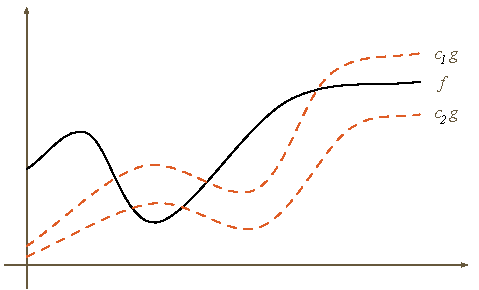
\includegraphics[scale=.5]{figures/asymptotic-theta.pdf}
    \end{figure}
%
  \end{itemize}
%
\end{frame}

% --------------------------------------
% upper and lower bounds
\begin{frame}[fragile]
%
  \frametitle{Upper and lower bounds}
%
  \begin{itemize}
%
  \item bounded from above: we say that $f = O(g)$ if there is a constant $c$ such that 
    $f(n) \leq c g(n)$ for sufficiently large $n$
%
    \begin{figure}
      \centering
      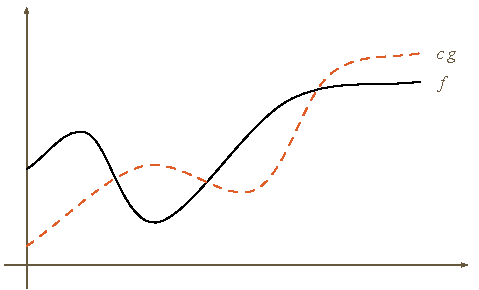
\includegraphics[scale=.5]{figures/asymptotic-o.pdf}
    \end{figure}
%
  \item bounded from below: we say that $f = \Omega(g)$ if there is a constant $c$ such that 
    $c g(n) \leq f(n)$ for sufficiently large $n$
%
    \begin{figure}
      \centering
      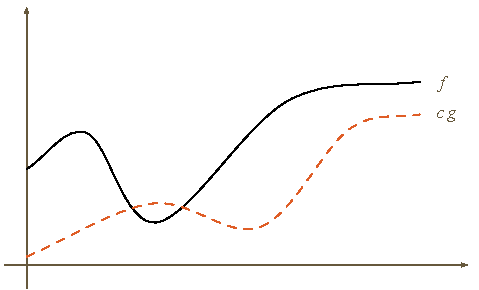
\includegraphics[scale=.5]{figures/asymptotic-omega.pdf}
    \end{figure}
%
  \end{itemize}
%
\end{frame}

% --------------------------------------
% algorithm design strategies
\begin{frame}[fragile]
%
  \frametitle{Designing algorithms}
%
  \begin{itemize}
%
  \item \insertionsort\ is {\em incremental}:
    \begin{itemize}
      \item having sorted $S[i..j]$, put $S[j]$ in its proper place
      \item how would you break this up into tasks that can be executed in parallel?
    \end{itemize}
%
  \item one alternative is {\em divide-and-conquer}: \mergesort
    \begin{itemize}
      \item {\em divide}: split $S$ into two parts of roughly equal length
      \item {\em conquer}: sort the subsequences recursively
      \item {\em combine}: merge the two sorted subsequences to produce the sorted output
    \end{itemize}
%
  \end{itemize}
%
\end{frame}

% --------------------------------------
% merge sort
\begin{frame}[fragile]
%
  \frametitle{Sorting by divide-and-conquer}
%
    \begin{center}
      \begin{minipage}{.75\linewidth}
        \begin{algorithm}[H]
          \label{alg:merge-sort}
%
          \DontPrintSemicolon
          %\NoCaptionOfAlgo
          \SetAlCapHSkip{0ex}
%
          \caption{\mergesort($S$, $p$, $r$)}
          \vspace{.5em}
%
          \If{$p < r$}{
            $q \leftarrow \lfloor (p+r)/2 \rfloor$ \;
            \mergesort($S$, $p$, $q$) \;
            \mergesort($S$, $q+1$, $r$) \;
            \merge($S$, $p$, $q$, $r$) \;
          }
%
          \vspace{.5em}
%
        \end{algorithm}
      \end{minipage}
    \end{center}
%
  \begin{itemize}
%
  \item {\em exercise}: write \merge; can be done in $\Theta(r-p+1)$
%
  \item analysis of running time:
    \begin{itemize}
    \item involves solving a recurrence relation
    \item worst case:
      \[
      T(n) = \left\{
      \begin{array}{ll}
        \Theta(1)         & {\rm if\ } n = 1 \\
        2T(n/2)+\Theta(n) & {\rm if\ } n > 1
      \end{array} \right\}
      \rightarrow \Theta(n \log n)
      \]
    \end{itemize}
%
  \item is this a better candidate for parallel sorting?
%
  \end{itemize}
%
\end{frame}

% end of file 

%% -*- LaTeX -*-
% -*- coding: utf-8 -*-
%
% michael a.g. aïvázis
% california institute of technology
% (c) 1998-2012 all rights reserved
%

\lecture{Survival skills meeting}{20120106}

% --------------------------------------
% bazaar
\begin{frame}[fragile]
%
  \frametitle{Bazaar -- setup}
%
  \begin{itemize}
%
  \item we are going to use \bzr, a source control system, for both homework and final project
    submissions
%
  \item installation instructions, documentation and tutorials available from
    \href{http://bazaar.canonical.com}
%
  \item bazaar keeps track of authors in its revision history, so it's a good idea to give it
    your name and an email address
%
    \begin{shell}{}
#> bzr whoami "Michael Aivazis <aivazis@caltech.edu>"
    \end{shell}
%
    \item you should verify that it worked by asking
%
   \begin{shell}{}
#> bzr whoami
Michael Aivazis <aivazis@caltech.edu>
    \end{shell}
%
  \end{itemize}
%
\end{frame}

% --------------------------------------
% bazaar
\begin{frame}[fragile]
%
  \frametitle{Bazaar -- brances}
%
  \begin{itemize}
%
  \item make a {\em branch} of the course repository by
%
    \begin{shell}{}
#> bzr branch http://acm114.caltech.edu/repository acm114
Branched 114 revision(s).
    \end{shell}
%
  \item you can look at history with the {\tt\small\bfseries log} command
%
    \begin{shell}{}
#> bzr log -l10 --line
114: Michael Aivazis 2010-01-14 Started fleshing out 2010.01.15
113: Michael Aivazis 2010-01-14 Posted an updated hw 2010.01.20 with some typos fixed
112: Michael Aivazis 2010-01-13 Created a stub for lecture 2010.01.15
111: Michael Aivazis 2010-01-13 Cosmetics to the reduction parallel work figure
110: Michael Aivazis 2010-01-13 Sidebar cosmetics
109: Michael Aivazis 2010-01-13 Cosmetics on the home page
108: Michael Aivazis 2010-01-13 Cosmetics on the news section of the home page
107: Michael Aivazis 2010-01-13 Published the updated 2010.01.13
106: Michael Aivazis 2010-01-13 Fixed a typo in 2010.01.13
105: Michael Aivazis 2010-01-13 Added news section to the home page
    \end{shell}
%
  \end{itemize}
%
\end{frame}

% --------------------------------------
% template
\begin{frame}[fragile]
%
  \frametitle{Blank}
%
  \begin{itemize}
%
  \item 
    \begin{itemize}
      \item
    \end{itemize}
%
  \end{itemize}
%
\end{frame}

% end of file 

%% -*- LaTeX -*-
% -*- coding: utf-8 -*-
%
% michael a.g. aïvázis
% california institute of technology
% (c) 1998-2012 all rights reserved
%

\lecture{Overview of parallel systems}{20120111}

% --------------------------------------
% motivation for parallel computing
\begin{frame}[fragile]
%
  \frametitle{Motivations for going parallel}
%
  \begin{itemize}
%
  \item why bother?
    \begin{itemize}
    \item {\em speed}: there are fundamental limits to the processing power of a single processor
    \item {\em throughput}: time to solution is critical for many problems
    \item {\em size}: high resolution requires lots of memory
    \item {\em availability}: the tool exists, use it
    \end{itemize}
%
  \item but be careful
    \begin{itemize}
    \item the commercial market is unstable
    \item the computing environment is somewhat primitive
    \item software packages and libraries are emerging slowly
    \item parallel programming is not hard, but it requires {\em discipline}
    \end{itemize}
%
  \end{itemize}
%
\end{frame}

% --------------------------------------
% computer system taxonomy
\begin{frame}[fragile]
%
  \frametitle{Taxonomy}
%
  \begin{itemize}
%
  \item an early classification of computer systems focussed on the relation between {\em
    instruction streams} and {\em data streams}:
    \begin{itemize}
      \item SISD: single instruction, single data
      \item SIMD: single instruction, multiple data
      \item MIMD: multiple instruction, multiple data
    \end{itemize}
%
    \item SISD describes conventional serial computers
    \begin{itemize}
      \item the programming model only: the hardware has moved on...
    \end{itemize}
%
    \item SIMD and MIMD are the traditional models for parallel machines
%
    \item MIMD systems are often programmed in SPMD mode: single {\em program}, multiple data
      \begin{itemize}
      \item when the parallel environment provides a {\em naming scheme} for the instruction
        streams, such as processor id, or task name
      \end{itemize}
  \end{itemize}
%
\end{frame}

% --------------------------------------
% architectural issues
\begin{frame}[fragile]
%
  \frametitle{Architectural issues}
%
  \begin{itemize}
%
  \item {\em control:} SIMD vs.~MIMD
  \item {\em co\"ordination}: synchronous vs.~asynchronous
  \item {\em memory organization}: private vs.~shared
  \item {\em address space}: local vs.~global
  \item {\em memory access}: uniform vs.~non-uniform
  \item {\em granularity}: the power of each processor
  \item {\em scalability}: dependence on the number of processors
  \item {\em interconnect}: topology, routing, switching
%
  \end{itemize}
%
\end{frame}

% --------------------------------------
% tradeoffs
\begin{frame}[fragile]
%
  \frametitle{Tradeoffs}
%
  \begin{center}
    \begin{minipage}{.75\linewidth}
      \begin{tabular}{l|l|l}
                        & shared memory & distributed memory \\ \hline
        scalability     & {\em harder}  & {\em easier} \\
        programmability & {\em easier}  & {\em harder}
      \end{tabular}
    \end{minipage}
  \end{center}

%
  \begin{itemize}
%
  \item shared memory permits parallelizing serial program gradually, focussing on worst
    bottlenecks first
%
  \item distributed memory requires partitioning and distributing both data and work across
    processors, which usually rules out incremental parallelization
%
  \end{itemize}
%
\end{frame}

% --------------------------------------
% categories of parallel architectures
\begin{frame}[fragile]
%
  \frametitle{Categories of parallel architectures}
%
  \begin{itemize}
%
  \item vector or array processor
  \item SMP: symmetric multiprocessor
  \item MPP: massively parallel multiprocessor
  \item DSM: distributed shared memory
  \item clusters
  \item hybrids
    \begin{itemize}
      \item SMP or MPP with vector processors
      \item networked clusters of SMPs
      \item SMP+GPGPU 
    \end{itemize}
%
  \end{itemize}
%
\end{frame}

% --------------------------------------
% generic parallel architecture
\begin{frame}[fragile]
%
  \frametitle{Generic parallel architecture}
%
  \begin{figure}
    \centering
    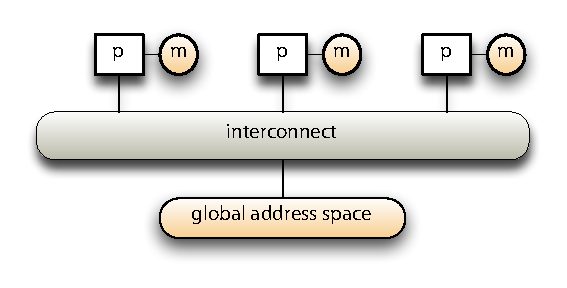
\includegraphics[width=.75\linewidth]{figures/generic-parallel-architecture.pdf}
    \label{fig:generic-parallel-architecture}
  \end{figure}

  \begin{itemize}
%
  \item a trivial but powerful observation: access to memory implies access to information
  \item hence, it becomes a determining factor for both hardware and algorithm design
%
  \end{itemize}
%
\end{frame}

% --------------------------------------
% memory hierarchy
\begin{frame}[fragile]
%
  \frametitle{Memory hierarchy}
%
  \begin{itemize}
  \item high performance architectures have a multi-tier memory hierarchy
%
    \begin{itemize}
    \item registers
    \item on-chip caches, usually referred to as level 1
    \item off-chip caches (level 2)
    \item random access memory
    \item remote memory (off processor)
    \item virtual memory, known as paging memory, that usually involves secondary storage
    \item secondary storage (disks)
    \item tertiary storage (tapes)
    \end{itemize}
%
  \item these have latencies and bandwidths that vary by orders of magnitude
  \item {\em cache misses} are the most frequently cited reason why real codes only achieve a
    small fraction of the benchmarked performance of a CPU
    \begin{itemize}
    \item really small: 10\% of peak is considered a success!
    \end{itemize}
%
  \end{itemize}
%
\end{frame}

% --------------------------------------
% parallel programming paradigms
\begin{frame}[fragile]
%
  \frametitle{Parallel programming paradigms}
%
  \begin{itemize}
%
  \item {\em functional languages}: specify what to compute, not how
  \item {\em parallelizing compilers}: automatic or semi-automatic detection of parallelism in
    serial code; mostly loop-unrolling, often with the help of special mark up (pragmas)
  \item {\em object oriented}: parallelism encapsulated within distributed objects

  \item {\em data parallel}: simultaneous operations on memory; mostly arrays
  \item {\em shared memory}: multiple threads executing a pool of tasks using common memory
  \item {\em remote memory access}: one sided put/get communication between processes
  \item {\em message passing}: two sided, co\"ordinated send/receive communication between
    processes
%
  \end{itemize}
%
\end{frame}

% --------------------------------------
% designing parallel algorithms
\begin{frame}[fragile]
%
  \frametitle{Designing parallel algorithms}
%
  \begin{itemize}
%
  \item {\em identification}: identify the part of the problem that can be parallelized
  \item {\em partition}: decompose the parallelizable part into fine-grained tasks
  \item {\em communication}: determine the necessary communication patterns among tasks
  \item {\em coarsening}: combine into coarser tasks and adjust the communication patterns
  \item {\em task mapping}: assign tasks to processors
%
  \end{itemize}
%
  \begin{figure}
    \centering
    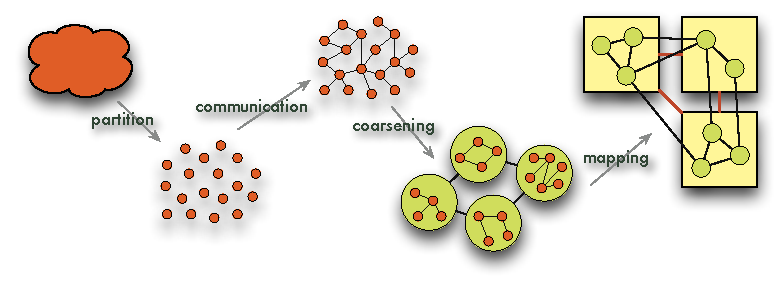
\includegraphics[scale=0.75]{figures/parallelization-steps.pdf}
    \label{fig:parallelization-steps}
  \end{figure}
%
\end{frame}

% --------------------------------------
% paradigms for parallel algorithms
\begin{frame}[fragile]
%
  \frametitle{Paradigms for parallel algorithms}
%
  \begin{itemize}
%
  \item {\em embarrassingly parallel}: mostly independent tasks
  \item {\em functional decomposition}: based on computational task (activity)
  \item {\em data parallel}: aka {\em loop-level} parallelism: array operations
  \item {\em domain decomposition}: based on the distribution of data
  \item {\em divide-and-conquer}: tree-like partitioning
  \item {\em pipelining}: multiple overlapping stages
%
  \end{itemize}
%
\end{frame}

% --------------------------------------
% communication issues
\begin{frame}[fragile]
%
  \frametitle{Communication issues}
%
  \begin{itemize}
%
  \item latency and bandwidth
  \item routing and switching -- not much of an issue any more
  \item contention, flow control and aggregate bandwidth
  \item collective communication
    \begin{itemize}
      \item one to many: broadcast, scatter
      \item many to one: gather, reduction, scan
      \item all to all
      \item synchronization barrier
    \end{itemize}
  \item assigning work to processors
    \begin{itemize}
    \item partitioning
    \item granularity
    \item mapping
    \item scheduling
    \item load balancing
    \end{itemize}
%
  \end{itemize}
%
\end{frame}

% --------------------------------------
% performance factors
\begin{frame}[fragile]
%
  \frametitle{Factors determining performance}
%
  \begin{itemize}
%
  \item {\em concurrency}: maximize the work that can be done in parallel
  \item {\em load balance}: make sure the load is (and stays) divided evenly
  \item {\em parallel overhead}: work not present in the equivalent serial computation
    \begin{itemize}
      \item process startup and shutdown costs
      \item communication
      \item synchronization
      \item redundancy
      \item speculative work
    \end{itemize}
%
  \end{itemize}
%
\end{frame}

% --------------------------------------
% computational models
\begin{frame}[fragile]
%
  \frametitle{Computational models}
%
  \begin{itemize}
%
    \item abstractions for architecture, algorithm analysis, and performance modeling
      \begin{itemize}
      \item PRAM: Parallel random access machine
      \item LogP: latency, overhead, gap, processors
      \item BSP: bulk synchronous parallel
      \item CSP: communicating sequential processes
      \item ... and many others
      \end{itemize}
%
    \item all occasionally useful tools for reasoning about implementation strategies for real
      programs, since they steer you away from common but perhaps non-obvious mistakes
    \item unfortunately, none is a substitute for understanding the characteristics of your
      target platform
%
  \end{itemize}
%
\end{frame}

% end of file 

%% -*- LaTeX -*-
% -*- coding: utf-8 -*-
%
% michael a.g. aïvázis
% california institute of technology
% (c) 1998-2012 all rights reserved
%

\lecture{Introduction to parallel programming models}{20120113}

% --------------------------------------
% generic parallel architecture
\begin{frame}[fragile]
%
  \frametitle{Impact of architecture on algorithm design}
%
  \begin{itemize}
%
    \item recall the five steps of parallel algorithm design
      \begin{itemize}
      \item identification of the parallelizable part, partitioning into fine grain tasks,
        examination of the task communication patterns, task coarsening, and mapping coarse
        tasks onto processors
      \end{itemize}
%
    \item and the layout of the generic parallel architecture:
%
  \begin{figure}
    \centering
    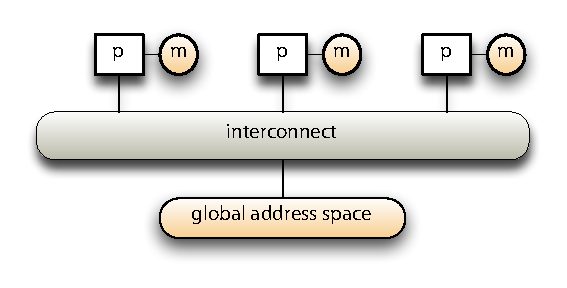
\includegraphics[width=.70\linewidth]{figures/generic-parallel-architecture.pdf}
    \label{fig:gpa-redux}
  \end{figure}
%
  \item let's move memory around and examine how this affects the programming model
  \item for a trivial but instructive problem
  \end{itemize}
%
\end{frame}

% --------------------------------------
% template
\begin{frame}[fragile]
%
  \frametitle{Parallel programming models}
%
  \begin{itemize}
%
  \item control
    \begin{itemize}
    \item how is parallelism {\em created}
    \item what is the {\em sequencing} of instruction streams in each task
    \item how do tasks {\em synchronize}
    \end{itemize}
%
    \item data address spaces
      \begin{itemize}
        \item what data is private to each task; what data must be shared
        \item how is logically shared data created, accessed or communicated, and synchronized
      \end{itemize}
%
    \item instruction sets
      \begin{itemize}
      \item what are the fundamental operations for process creation, communication,
        and synchronization
      \item which operations are {\em atomic}
      \end{itemize}
%
    \item cost
      \begin{itemize}
      \item how fast does it run
      \item are resources used efficiently
      \item how hard is it to code correctly
      \end{itemize}
%
  \end{itemize}
%
\end{frame}

% --------------------------------------
% problem setup
\begin{frame}[fragile]
%
  \frametitle{Embarrassingly parallel: $p$ processor reduction}
%
  \begin{itemize}
%
  \item given a function $f$ and a sequence of numbers $S$ of length $N$, evaluate the sum
    \[
    s = \sum_{i=0}^{N-1}f(S_{i})
    \]
%
  \item parallel tasks: the function evaluations, the computation of partial sums
%
  \item strategy: assign $n/p$ numbers to each processor
    \begin{itemize}
      \item each processor performs $n/p$ evaluations of $f$
      \item each processor computes its own partial sum
      \item one(?) of them collects the $p$ partial sums, and computes the global sum $s$
    \end{itemize}
%
  \item two classes of data
    \begin{itemize}
      \item logically shared:
        \begin{itemize}
        \item the global sum
        \item the input sequence $S$
        \end{itemize}
      \item logically private:
        \begin{itemize}
          \item the evaluations of $f$ on the local subsequence
          \item the local partial sums (?)
        \end{itemize}
    \end{itemize}
%
  \end{itemize}
%
\end{frame}

% --------------------------------------
% machine model 1: a shared memory machine
\begin{frame}[fragile]
%
  \frametitle{Shared memory machines}
%
  \begin{itemize}
%
  \item processors are all connected to a large pool of shared memory with a global address
    space
  \item typically, each processor has some local cache, but no private memory
  \item {\em cost}: accessing the cache is {\em much} faster than main memory
    \begin{itemize}
      \item tune: the memory footprint of $n/p$ numbers should match cache size
    \end{itemize}
%
  \begin{figure}
    \centering
    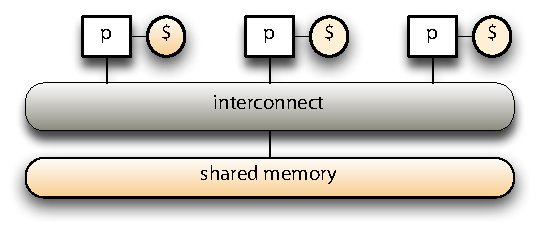
\includegraphics[width=.70\linewidth]{figures/shared-memory.pdf}
    \label{fig:shared-memory}
  \end{figure}
%
  \item for shared {\em address space} machine:
    \begin{itemize}
      \item replace caches with local/private memory
      \item cost: repeatedly accessed data should be copied to local storage
      \item not done much any more, but recently relevant thanks to hybrid CPU/GPGPU systems and
        the implementation details of nVidia chips
    \end{itemize}
%
  \end{itemize}
%
\end{frame}

% --------------------------------------
% programming a shared memory machine
\begin{frame}[fragile]
%
  \frametitle{Programming in a shared address space}
%
  \begin{itemize}
%
  \item the program creates and manages $p$ instruction streams (threads)
  \item each with a set of private variables
    \begin{itemize}
      \item registers, stack, cache
    \end{itemize}
%
  \item collectively with a set of shared variables
    \begin{itemize}
      \item statics, heap
    \end{itemize}
%
  \item communication is {\em implicit}: threads just access the shared memory locations
  \item synchronization is {\em explicit}: read/write flags, locks, semaphores
%
  \begin{figure}
    \centering
    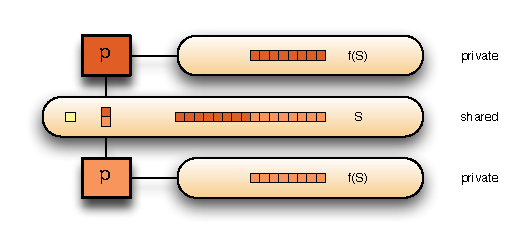
\includegraphics[width=\linewidth]{figures/reduction-shared.pdf}
    \label{fig:reduction-shared}
  \end{figure}
%
  \end{itemize}
%
\end{frame}

% --------------------------------------
% implementation of the reduction in a shared memory machine
\begin{frame}[fragile]
%
  \frametitle{Implementation in a shared address space}
%
  \begin{itemize}
%
  \item let's implement with two threads

    \vspace{.5em}
    \begin{minipage}{.40\linewidth}
      \begin{algorithm}[H]
%
        \footnotesize
        \DontPrintSemicolon
        \NoCaptionOfAlgo
        \SetAlCapHSkip{0ex}
%
        \caption{\hspace{1em}thread 1}
        \vspace{.5em}
%
        $s \leftarrow 0$ \;
        $s_{1} \leftarrow 0$ \;
        \For{$i \leftarrow 1$ \KwTo $n/2-1$}{
          $s_{1} \leftarrow s_{1} + f(S[i])$ \;
        }
        $s \leftarrow s+s_{1}$ \;
%
        \vspace{.5em}
%
      \end{algorithm}
    \end{minipage}
%
    \hspace{.1\linewidth}
%
    \begin{minipage}{.40\linewidth}
      \begin{algorithm}[H]
%
        \footnotesize
        \DontPrintSemicolon
        \NoCaptionOfAlgo
        \SetAlCapHSkip{0ex}
%
        \caption{\hspace{1em}thread 2}
        \vspace{.5em}
%
        $s \leftarrow 0$ \;
        $s_{2} \leftarrow 0$ \;
        \For{$i \leftarrow n/2$ \KwTo $n$}{
          $s_{2} \leftarrow s_{2} + f(S[i])$ \;
        }
        $s \leftarrow s+s_{2}$ \;
%
        \vspace{.5em}
      %
      \end{algorithm}
    \end{minipage}
    \vspace{.5em}
%
  \item what is wrong with this code? 
%
    \begin{itemize}
    \item {\em race condition}
    \item instructions from different threads can be executed in any order
    \item can you deduce all the possible values of $s$ after both threads finished executing?
    \item one possible solution is to place line 5 in a lock/load/modify/store/unlock block
    \end{itemize}
%
  \end{itemize}
%
\end{frame}

% --------------------------------------
% machine model 2: a distributed memory machine
\begin{frame}[fragile]
%
  \frametitle{Distributed memory machines}
%
  \begin{itemize}
%
  \item processors are all connected to their own private memory
  \item processors have no access to each other's memory, except through explicit exchanges
  \item each node is connected to a communication substrate: ethernet, myrinet, infiniband
%
  \begin{figure}
    \centering
    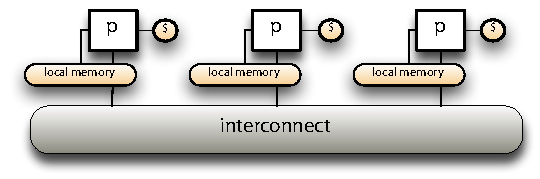
\includegraphics[width=.90\linewidth]{figures/distributed-memory.pdf}
    \label{fig:distributed-memory}
  \end{figure}
%
  \item all communication and synchronization is carried over the interconnect 
%
  \end{itemize}
%
\end{frame}

% --------------------------------------
% programming a distributed memory machine
\begin{frame}[fragile]
%
  \frametitle{Programming in a distributed address space}
%
  \begin{itemize}
%
  \item message passing
    \begin{itemize}
      \item programs consists of a collection of $n$ {\em named} processes
        \begin{itemize}
        \item typically numbered 0 through $n-1$
        \item thread of control, local address space
        \item local variables, statics, heap
        \end{itemize}
      \item processes communicate via {\em explicit} data exchanges
        \begin{itemize}
        \item matching pair of send/receive by source and destination processors respectively
        \item primitives for efficient implementation of many-to-many exchanges
        \end{itemize}
      \item co\"ordination is implicit in every communication
      \item logically shared data must be {\em partitioned} among the local processes
    \end{itemize}
%
  \item standard libraries: MPI, the survivor
%
  \begin{figure}
    \centering
    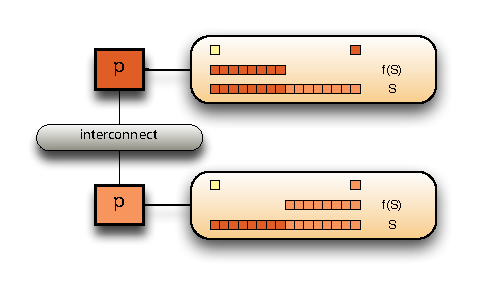
\includegraphics[width=.5\linewidth]{figures/reduction-distributed.pdf}
    \label{fig:reduction-distributed}
  \end{figure}
%
  \end{itemize}
%
\end{frame}

% --------------------------------------
% implementation of the reduction in a distributed memory machine
\begin{frame}[fragile]
%
  \frametitle{Implementation in a distributed address space}
%
  \begin{itemize}
%
  \item na\"ive implementation

    \vspace{.5em}
    \begin{minipage}{.40\linewidth}
      \begin{algorithm}[H]
%
        \footnotesize
        \DontPrintSemicolon
        \NoCaptionOfAlgo
        \SetAlCapHSkip{0ex}
%
        \caption{\hspace{1em}processor 1}
        \vspace{.5em}
%
        $s_{1} \leftarrow 0$ \;
        \For{$i \leftarrow 1$ \KwTo $n/2-1$}{
          $s_{1} \leftarrow s_{1} + f(S[i])$ \;
        }
        \KwSend $s_{1}$ \KwTo $p_{2}$ \;
        $s_{2} \leftarrow \KwRecv\ \KwFrom\ p_{2}$ \;
        $s \leftarrow s_{1}+s_{2}$ \;
%
        \vspace{.5em}
%
      \end{algorithm}
    \end{minipage}
%
    \hspace{.1\linewidth}
%
    \begin{minipage}{.40\linewidth}
      \begin{algorithm}[H]
%
        \footnotesize
        \DontPrintSemicolon
        \NoCaptionOfAlgo
        \SetAlCapHSkip{0ex}
%
        \caption{\hspace{1em}processor 2}
        \vspace{.5em}
%
        $s_{2} \leftarrow 0$ \;
        \For{$i \leftarrow n/2$ \KwTo $n$}{
          $s_{2} \leftarrow s_{2} + f(S[i])$ \;
        }
        \KwSend $s_{2}$ \KwTo $p_{1}$ \;
        $s_{1} \leftarrow \KwRecv\ \KwFrom\ p_{1}$ \;
        $s \leftarrow s_{2}+s_{1}$ \;
%
        \vspace{.5em}
      %
      \end{algorithm}
    \end{minipage}
    \vspace{.5em}
%
  \item what is wrong with this code? 
%
    \begin{itemize}
    \item {\em race condition}; more subtle than before
    \item send may block until a matching receive is executed  
    \end{itemize}
  \item options:
    \begin{itemize}
    \item pair up sends and receives to create logically atomic exchanges
    \item use non-blocking or asynchronous primitives
    \item use a many-to-many communication primitive, if available
    \end{itemize}
%
  \end{itemize}
%
\end{frame}

% --------------------------------------
% machine model 3: SIMD
\begin{frame}[fragile]
%
  \frametitle{SIMD machines}
%
  \begin{itemize}
%
  \item a large number of small, special purpose processors
%
  \item a single ``controller'' manages the instruction stream
    \begin{itemize}
      \item each processor executes the same instruction on its local data
      \item may be able  to specify which processors are active/idle
    \end{itemize}
%
  \begin{figure}
    \centering
    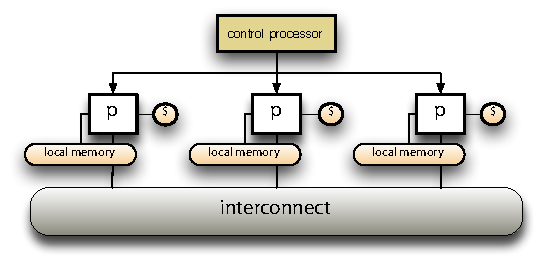
\includegraphics[width=.70\linewidth]{figures/simd.pdf}
    \label{fig:simd}
  \end{figure}
%
  \item hardware of this type fell out favor years ago
    \begin{itemize}
      \item but the associated programming model is still popular
      \item implemented by mapping $n$-fold parallelism to $p$ processors
      \item mostly done by compilers, e.g.~{\em High Performance FORTRAN} (HPF)
    \end{itemize}
%
  \item relevant again thanks to the CPU+GPGPU hybrids, which have similar layout
%
  \end{itemize}
%
\end{frame}

% --------------------------------------
% programming a SIMD machine
\begin{frame}[fragile]
%
  \frametitle{Data parallel programming model}
%
  \begin{itemize}
%
  \item single instruction stream of {\em parallel} operations
  \item parallel operation applied to entire data structure
    \begin{itemize}
      \item you may be able to restrict the {\em range} of operations to some defined subset of
        the data
    \end{itemize}
  \item communication and synchronization are implicit in the definition of the parallel
    operators
%
  \begin{figure}
    \centering
    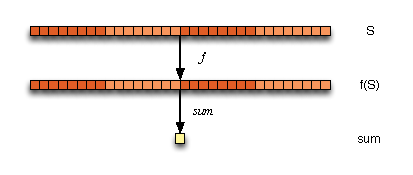
\includegraphics[scale=1.0]{figures/reduction-simd.pdf}
    \label{fig:reduction-simd}
  \end{figure}
%
  \item rather elegant, easy to understand, easy to reason about
  \item unfortunately, not all problems fit the paradigm nicely
  \item implemented by parallel functional languages, MATLAB
%
  \end{itemize}
%
\end{frame}

% --------------------------------------
% machine model 4: clusters
\begin{frame}[fragile]
%
  \frametitle{Clusters}
%
  \begin{itemize}
%
  \item commodity hardware configurations:
    \begin{itemize}
      \item CPUs with multiple cores: $2 \rightarrow 4 \rightarrow 6 \rightarrow 8 \rightarrow
        ?$
      \item motherboards with multiple CPUs
      \item sizeable memory on a single board
    \end{itemize}
%
  \item this hybrid is the current mainstream deployment: most of the Top500
%
  \item shared memory within a {\em blade}, message passing across blades
%
  \item there had to be an acronym: CLUMPs; fortunately no one uses it...
%
  \item programming models:
    \begin{itemize}
      \item treat machine as flat and always use message passing
        \begin{itemize}
        \item simple but ignores the performance characteristics of the memory hierarchy
        \item message passing library may be smart enough to switch between network and shared
          memory dynamically, e.g.~openMPI
        \end{itemize}
      \item expose both layers explicitly
        \begin{itemize}
          \item higher performance, but unpleasant to program
          \item hard to make portable
        \end{itemize}
    \end{itemize}
%
  \end{itemize}
%
\end{frame}

% --------------------------------------
% programming model 5: bulk synchronous
\begin{frame}[fragile]
%
  \frametitle{Bulk synchronous programming model}
%
  \begin{itemize}
%
  \item strategy that applies to both shared memory and message passing programming models
%
  \item program consists of interleaved {\em phases} synchronized by global barriers
    \begin{itemize}
      \item {\em compute} phases: all processors 
        \begin{itemize}
          \item operate on local data -- distributed memory
          \item operate with read access to global data -- shared memory
        \end{itemize}
      \item {\em communication} phases: all processors participate in data exchanges,
        rearrangements or reductions of global data
    \end{itemize}
%
    \item single program multiple data
      \begin{itemize}
        \item everybody is doing the same thing
        \item maps well to the structure of solutions of PDEs
          \begin{itemize}
            \item exchange data on processor partition boundaries 
            \item apply boundary conditions
            \item agree on a stable $\Delta t$ size (a global reduction)
            \item advance the solution by $\Delta t$
            \item repeat until you run out of time...
          \end{itemize}
      \end{itemize}
%
  \end{itemize}
%
\end{frame}

% --------------------------------------
% summary
\begin{frame}[fragile]
%
  \frametitle{Recap}
%
  \begin{itemize}
%
  \item in the early days, each machine was unique
    \begin{itemize}
      \item hardware, support for one programming model, perhaps a dedicated language with its
        compiler
%
      \item when a new machine came out you had to throw all your code away and start again
        \begin{itemize}
        \item ok for getting a thesis out, bad for building a career
        \end{itemize}
    \end{itemize}
%
  \item now we distinguish the programming model from the underlying hardware, so we can write
    portable, {\em correct} code that runs on large classes of machines
%
  \item unfortunately, writing {\em fast} code still requires tuning for some architectural
    details
    \begin{itemize}
      \item the design challenge is to simplify this process
      \item e.g., by exposing these details as user-configurable options that are determined at
        run-time
      \item best handled by {\em application frameworks}
    \end{itemize}
%
  \end{itemize}
%
\end{frame}

% --------------------------------------
% parallelization steps
\begin{frame}[fragile]
%
  \frametitle{Parallelization steps}
%
  \begin{figure}
    \centering
    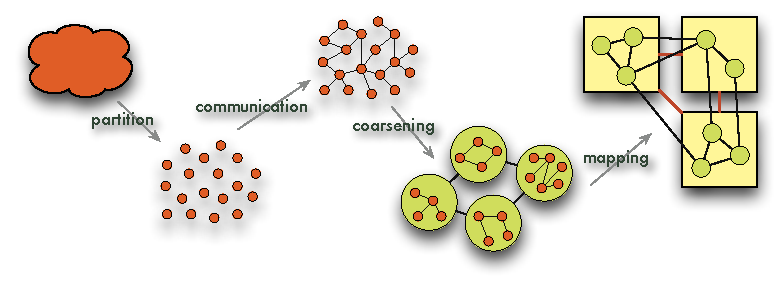
\includegraphics[scale=0.75]{figures/parallelization-steps.pdf}
    \label{fig:parallelization-steps}
  \end{figure}
  \vspace{-3.0em}
%
  \begin{itemize}
%
    \item steps in creating a parallel program
      \begin{itemize}
      \item identify the work that can be done in parallel
      \item partition it in terms of work units, the fine grain tasks
      \item analyze the communication patterns among work units
      \item coarsen into processes, the abstract entities that carry out tasks
      \item map to processors, the physical entities that execute the processes
      \end{itemize}
%
    \item goal: maximize the speedup due to parallelism
%
  \end{itemize}
%
\end{frame}

% --------------------------------------
% parallelizing reduction
\begin{frame}[fragile]
%
  \frametitle{Parallelizing our reduction example}
%
  \begin{itemize}
%
    \item for our example $s = \sum f(S)$
    \item partition into tasks
      \begin{itemize}
      \item computing each of the $F(S_{i})$
      \item $n$-fold parallelism, where ideally $n \gg p$ 
      \item computing the sum $s$
      \end{itemize}
%
    \item communication
      \begin{itemize}
        \item distribution of the initial input sequence $S$
        \item collection of the partial sums
      \end{itemize}
%
    \item coarsening: compute the partial sum of a cluster of evaluations
      \begin{itemize}
        \item thread $k$ sums up $s_{k} = \sum_{i = k n/p}^{(k+1)n/p 1} f(S_{i})$
        \item thread 1 sums up the partial results and communicates the result to the other
          threads
      \end{itemize}
%
    \item mapping: processor $i$ runs thread $i$
%
    \item at {\em runtime}
      \begin{itemize}
        \item start up the $p$ threads
        \item communicate/synchronize with thread 1
      \end{itemize}
%
  \end{itemize}
%
\end{frame}

% end of file 

%% -*- LaTeX -*-
% -*- coding: utf-8 -*-
%
% ~~~~~~~~~~~~~~~~~~~~~~~~~~~~~~~~~~~~~~~~~~~~~~~~~~~~~~~~~~~~~~~~~~~~~~~~~~~~~~
%
%                             michael a.g. aïvázis
%                      california institute of technology
%                      (c) 1998-2010  all rights reserved
%
% ~~~~~~~~~~~~~~~~~~~~~~~~~~~~~~~~~~~~~~~~~~~~~~~~~~~~~~~~~~~~~~~~~~~~~~~~~~~~~~
%

\lecture{Programming with pthreads}{20100120}

% --------------------------------------
% threads and shared memory parallelism 
\begin{frame}[fragile]
%
  \frametitle{Threads and shared memory parallelism}
%
  \begin{itemize}
%
  \item recall the shared memory architecture
%
    \begin{figure}
      \centering
      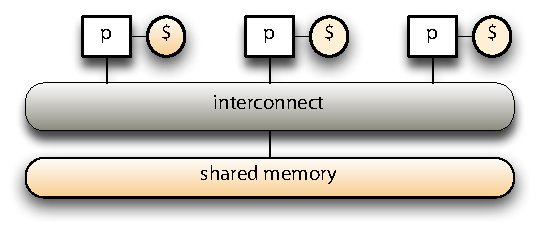
\includegraphics[scale=0.5]{figures/shared-memory.pdf}
    \end{figure}
    \vspace{-1.0em}
%
    \begin{itemize}
    \item processors are connected to a memory pool with a global address space
    \item processors have their own cache but no private memory
    \end{itemize}
%
  \item model is relevant for {\em threads}
%
    \begin{itemize}
    \item lightweight processes that can be scheduled independently, but share many OS
      resources
      \begin{itemize}
      \item CPU
      \item memory
      \item but also file descriptors, process environment, etc.
      \end{itemize}
    \item supported by most modern operating systems
    \end{itemize}
%
  \end{itemize}
%
    \begin{figure}
      \centering
      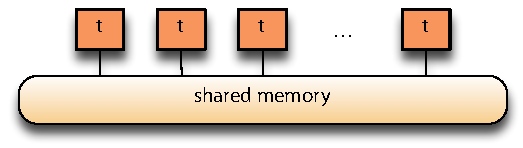
\includegraphics[scale=0.5]{figures/threads-memory.pdf}
    \end{figure}
%
\end{frame}

% --------------------------------------
% template
\begin{frame}[fragile]
%
  \frametitle{Processes and threads}
%
  \begin{itemize}
%
  \item in most operating systems, a process has
    \begin{itemize}
    \item process id and group id, user id and group id
    \item environment variables
    \item working directory
    \item scheduling information
    \item registers, stack, heap, instruction stream
    \item file descriptors, signal handlers, other process dependent structures
    \end{itemize}
%
  \item threads 
    \begin{itemize}
      \item share many of the per-process properties
        \begin{itemize}
        \item they are lightweight since they incur low overhead
        \end{itemize}
      \item have their own copy of
        \begin{itemize}
        \item registers, stack, instruction stream
        \item scheduling information
        \end{itemize}
    \end{itemize}
%
  \item threads are important programming constructs
    \begin{itemize}
    \item every vendor supports a proprietary interface
    \item {\em pthreads}, the POSIX standard API specification brought portability
    \item standardized creation, management, synchronization
    \end{itemize}
%
  \end{itemize}
%
\end{frame}

% --------------------------------------
% template
\begin{frame}[fragile]
%
  \frametitle{The pthreads API}
%
  \begin{itemize}
%
  \item threads require support from the compiler, the linker, the loader, and the OS kernel
    \begin{itemize}
    \item thread safety
    \end{itemize}
%
  \item special command line argument to most compliant compilers
    \begin{itemize}
    \item changes the instruction strategy
    \item adds the pthread runtime library to the link line
    \item links against the thread safe runtime
    \end{itemize}
%
  \item naming conventions
    \begin{table}
      \scriptsize
      \centering
      \begin{tabular}{l|l}
        Prefix & Functional group\\ \hline
        {\tt pthread\_ } &
            access to the threads, and some miscellaneous routines\\
        {\tt pthread\_attr\_ } & 
            thread attribute objects\\
        {\tt pthread\_mutex\_ } & 
            mutexes\\
        {\tt pthread\_mutexattr\_ } & 
            mutex attribute objects\\
        {\tt pthread\_cond\_ } & 
            condition variables\\
        {\tt pthread\_condattr\_ } & 
            condition variable attribute objects\\
        {\tt pthread\_key\_ } & 
            thread-specific data keys\\
        {\tt pthread\_rwlock\_ } & 
            read/write locks\\
        {\tt pthread\_barrier\_ } & 
            synchronization barriers\\
      \end{tabular}
    \end{table}
%
  \item the standard specifies the API for \cc\ only; \fortran\ support varies
    \begin{itemize}
    \item must include \srcfile{pthread.h}
    \end{itemize}
%
  \item lots of good books; see \href{http://acm114.caltech.edu/references}
%
  \end{itemize}
%
\end{frame}

% --------------------------------------
% template
\begin{frame}[fragile]
%
  \frametitle{Creating threads}
  \begin{itemize}
%
  \item create threads by calling
%
  \begin{C}
int pthread_create(
    pthread_t* id, const pthread_attr_t* attr,
    void* (*startup)(void*), void* arg);
  \end{C}
%
\item initially a process has one thread; every other thread must be explicitly created
  by calling \function{pthread\_create} and passing
  \begin{itemize}
  \item \identifier{id}: the location where a unique thread identifier will be stored
  \item \identifier{attr}: an opaque attribute object with thread initialization options
  \item \function{startup}: a pointer to a \cc\ function that will be executed by the thread
    once it gets scheduled
  \item \identifier{arg}: user defined data to be passed to \function{startup}; may be \NULL
  \end{itemize}
%
  \item once scheduled, threads are first class citizens
%
  \item the maximum number of threads per process depends on the implementation
%
  \end{itemize}
%
    \begin{figure}
      \centering
      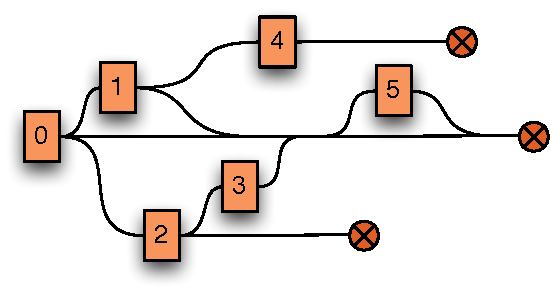
\includegraphics[scale=0.5]{figures/threads.pdf}
    \end{figure}
%
\end{frame}

% --------------------------------------
% terminating threads
\begin{frame}[fragile]
%
  \frametitle{Terminating threads}
%
  \begin{itemize}
%
    \item several ways to terminate a thread
      \begin{itemize}
      \item the thread returns from \function{main}
      \item the thread explicitly calls \function{pthread\_exit}
      \item the thread is killed when another thread calls \function{pthread\_cancel}
      \item the process terminates due to some system call, e.g.~\function{exit},
        \function{exec}, etc.
      \end{itemize}
%
  \item use \function{pthread\_exit} to kill a thread when it is no longer needed
%
    \begin{C}
int pthread_exit(void * status);
    \end{C}
%
  \item if \function{main} finishes and any threads remain
    \begin{itemize}
    \item they get killed unless \function{main} has called \function{pthread\_exit}
    \item otherwise they continue to run
    \end{itemize}
%
  \item thread routines do not have to call \function{pthread\_exit} unless they intend to pass
    their termination status to their creator
%
  \item \function{pthread\_exit} does not perform any process cleanup: it doesn't flush/close
    files, release other resources, signal the process parent, etc.
  \end{itemize}
%
\end{frame}

% --------------------------------------
% hello world
\begin{frame}[fragile]
%
  \frametitle{Hello world}
%
  \begin{C}
#include <pthread.h>
#include <stdio.h>
#define THREADS 10

void* hello(void* threadID) {
    long id = (long) threadID;
    printf("hello from %02ld/%0d\n", id, THREADS);
    pthread_exit(NULL);
    return NULL;
}

int main(int argc, char* argv[]) {
    long id;
    int status;
    pthread_t threads[THREADS];

    for (id=0; id<THREADS; id++) {
        printf("creating thread %02ld\n", id);
        status = pthread_create(&threads[id], NULL, hello, (void*) id);
        if (status) {
            printf("error %d in pthread_create\n", status);
        }
    }
    /* there is a problem here... */
    pthread_exit(NULL);
    return 0;
}
  \end{C}
%
\end{frame}

% end of file 

%% -*- LaTeX -*-
% -*- coding: utf-8 -*-
%
% ~~~~~~~~~~~~~~~~~~~~~~~~~~~~~~~~~~~~~~~~~~~~~~~~~~~~~~~~~~~~~~~~~~~~~~~~~~~~~~
%
%                             michael a.g. aïvázis
%                      california institute of technology
%                      (c) 1998-2010  all rights reserved
%
% ~~~~~~~~~~~~~~~~~~~~~~~~~~~~~~~~~~~~~~~~~~~~~~~~~~~~~~~~~~~~~~~~~~~~~~~~~~~~~~
%

\lecture{Cost modeling and performance tradeoffs}{20100113}

% --------------------------------------
% generic parallel architecture
\begin{frame}[fragile]
%
  \frametitle{Time, parallelism and computational work}
%
  \begin{itemize}
  \item recall our embarrassingly parallel reduction: 
    \begin{itemize}
    \item given a function $f$ and a sequence of numbers $S$ of length $N$, evaluate
    \[
    s = \sum_{i=0}^{N-1}f(S_{i})
    \]
    \end{itemize}
%
  \item initial parallelism profile for a simple mapping, assuming that
    \begin{itemize}
    \item the computation of $f(S)$ is the parallel task
    \item the summation is sequential
    \end{itemize}
%
    \begin{minipage}{.45\linewidth}
      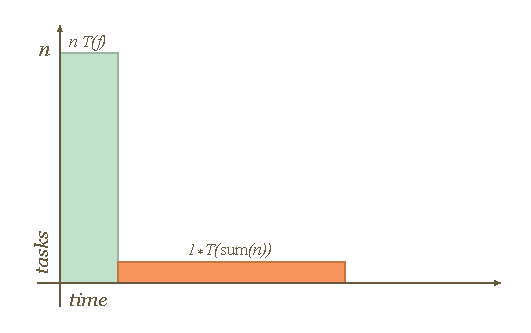
\includegraphics[scale=0.6]{figures/reduction-parallel-work.pdf}
    \end{minipage}
    $\longrightarrow$
    \begin{minipage}{.45\linewidth}
      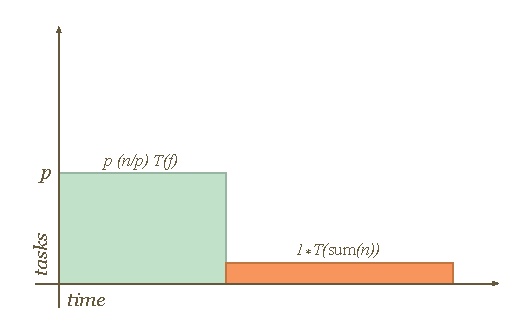
\includegraphics[scale=0.6]{figures/reduction-partitioned-work.pdf}
    \end{minipage}
%
  \item shaded area is $w$, the {\em computational work}
%
  \end{itemize}
%
\end{frame}

% --------------------------------------
% speedup and efficiency
\begin{frame}[fragile]
%
  \frametitle{Metrics: speedup and efficiency}
%
  \begin{itemize}
%
    \item let
      \begin{itemize}
        \item $T_{1}$ be the sequential execution time on one processor
        \item $T_{p}$ be the parallel execution time on $p$ processors
      \end{itemize}
%
    \item define
      \begin{itemize}
        \item {\em speedup}: \[\sigma \defeq T_{1}/T_{p}\]
        \item {\em efficiency}: \[\eta \defeq T_{1}/(p T_{p})\]
        \item related through $\eta = \sigma/p$ and $\sigma = \eta p$
      \end{itemize}
%
    \item pseudo-theorems: $\sigma \leq p$ and $\eta \leq 1$
      \begin{itemize}
        \item but {\em speedup anomalies} can occur if resources increase with $p$ causing an
          increase in the effective computation rate
        \item example: for large enough $p$, your problem may fit entirely in the L2 cache
        \item {\em sweet spots} like that abound; the craftsman knows how to
          \begin{itemize}
            \item implement the solution in a portable manner
            \item expose enough controls to enable tuning to a given architecture at {\em
              runtime}
          \end{itemize}
      \end{itemize}
%
  \end{itemize}
%
\end{frame}

% --------------------------------------
% amdahl's law
%
\begin{frame}[fragile]
%
  \frametitle{The bad news: Amdahl's law}
%
  \begin{minipage}{.55\linewidth}
    \begin{itemize}
%
    \item consider a solution that consists of two parts
      \begin{itemize}
      \item a serial fraction $s$ with $0 \leq s \leq 1$
      \item a $p$-fold parallel fraction $1-s$
      \end{itemize}
%
    \item for a fixed problem size, Amdahl's law relates $(T_{p}, \sigma, \eta)$ to
      $(T_{1}, s)$
      \begin{eqnarray*}
        T_{p}  & = & s T_{1} + (1-s) T_{1} / p \\
        \sigma & = & \frac{p}{sp + (1-s)} \\
        \eta & = & \frac{1}{sp + (1-s)}
      \end{eqnarray*}
%
    \item with corollaries $\sigma_{\infty} = \frac{1}{s}$ and $\eta_{\infty} = 0$
    \end{itemize}
  \end{minipage}
 %
  \hfill
  \begin{minipage}{.40\linewidth}
    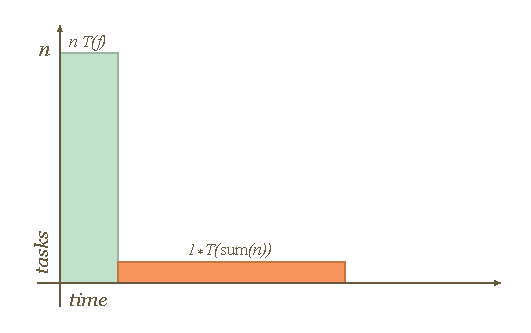
\includegraphics[width=1.2\linewidth]{figures/reduction-parallel-work.pdf}
    \vspace{2em}

    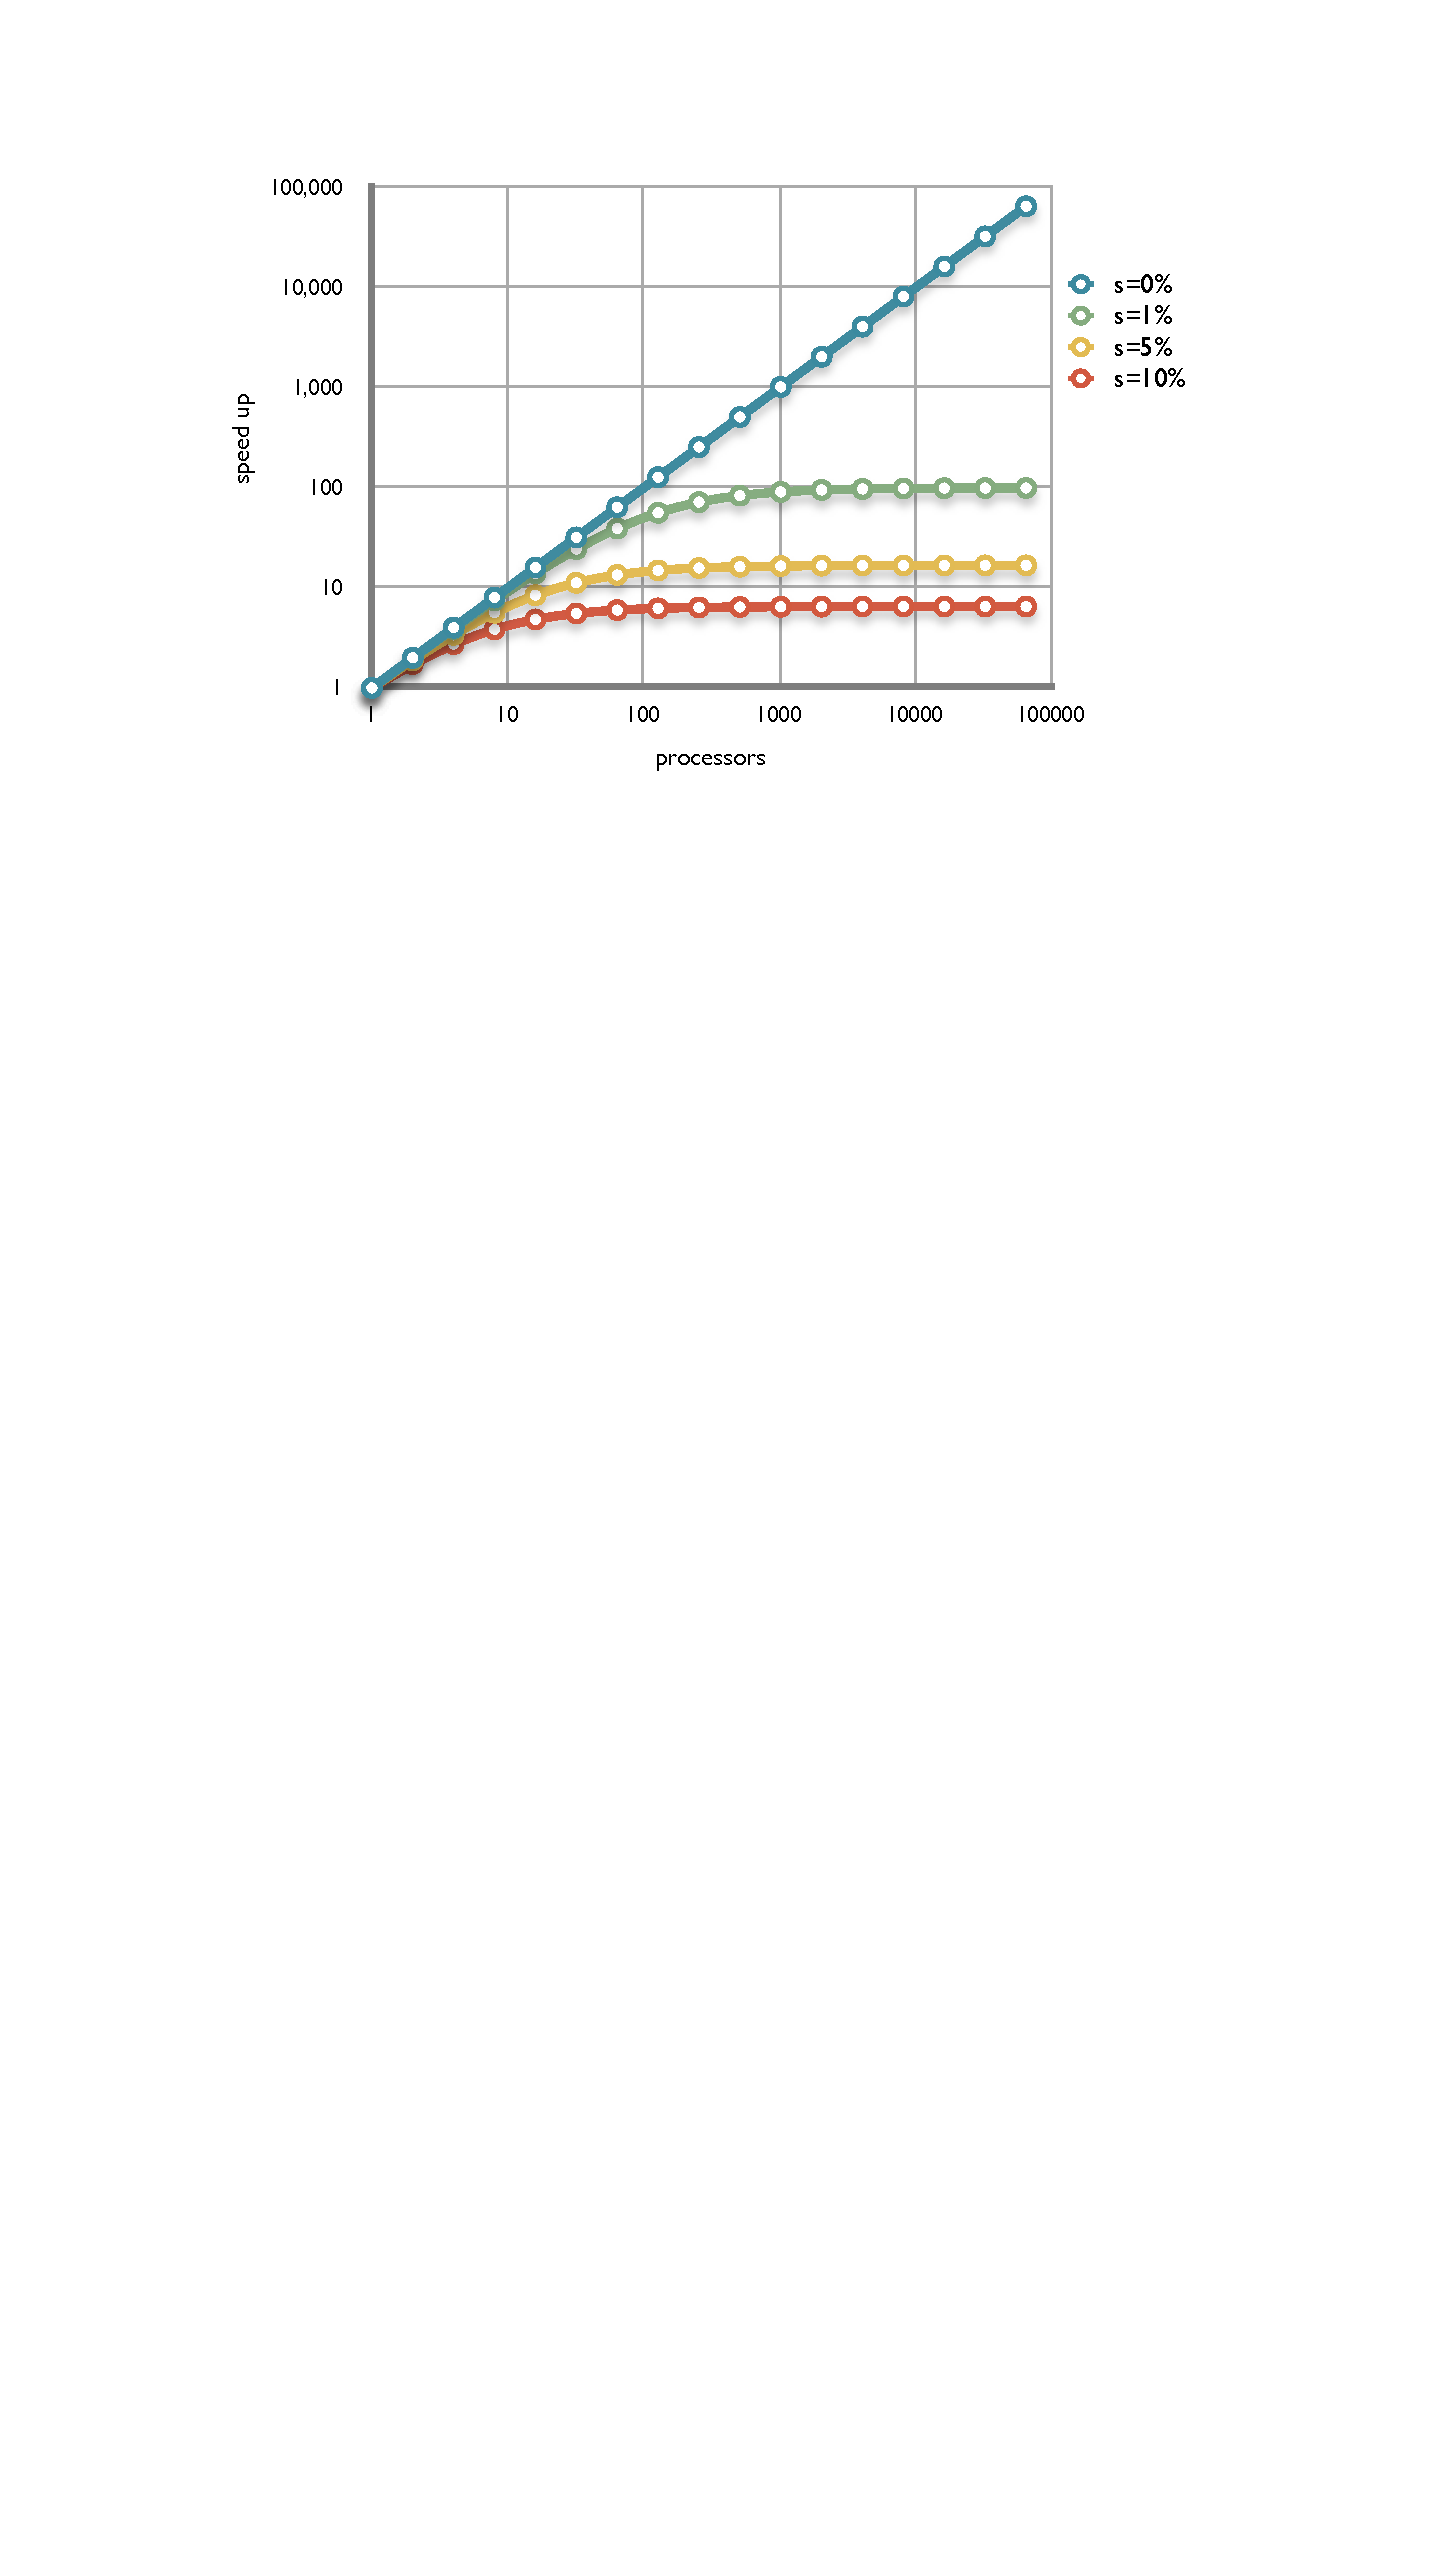
\includegraphics[width=1.2\linewidth]{figures/amdahl.pdf}
  \end{minipage}
%
\end{frame}

% --------------------------------------
% scaling and isoefficiency
\begin{frame}[fragile]
%
  \frametitle{Beating Amdahl's law}
%
  \begin{itemize}
  \item Amdahl's law holds if
    \begin{itemize}
      \item the problem size is fixed
      \item the serial fraction $s$ is not a function of $p$
    \end{itemize}
%
  \item {\em weak scaling}: let the problem size grow with $p$
    \begin{itemize}
    \item larger computers are used to solve larger problems
    \item the effective serial fraction {\em decreases} with problem size
    \item the right scaling metric would be constant, or properly bounded away from 0, as $p
      \rightarrow \infty$
    \end{itemize}
%
  \item {\em isoefficiency}
    \begin{itemize}
      \item how rapidly must the problem size grow so that $\eta$ is constant as $p$ increases?
      \item since $\eta = T_{1}/(pT_{p})$, constant efficiency implies
        \[
        T_{1} = c (p T_{p})
        \]
        for some constant $c$
      \item $T_{1}$ measures the sequential work, so the above relation determines your
        implementation's {\em isoefficiency function}
    \end{itemize}
%
  \end{itemize}
%
\end{frame}



% --------------------------------------
% algorithmic trade-offs
\begin{frame}[fragile]
%
  \frametitle{Algorithmic improvements}
%
  \begin{itemize}
%
  \item getting smarter is the best way to improve $\sigma$ and $\eta$
    \begin{itemize}
      \item reduce the sequential fraction $s$
      \item what are the effects on communication and locality?
    \end{itemize}
%
  \item parallelize the partial sums
    \begin{figure}
      \centering
      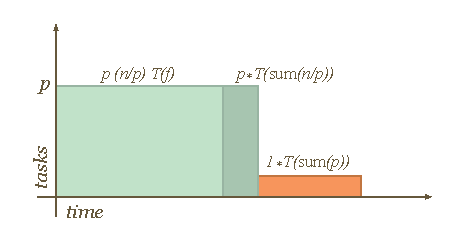
\includegraphics[scale=0.70]{figures/reduction-partial-sum.pdf}
    \end{figure}
%
  \item parallelize the final sum using a {\em reduction tree}
    \begin{figure}
      \centering
      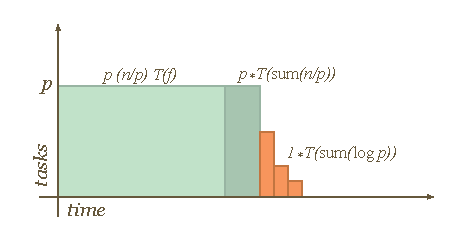
\includegraphics[scale=0.70]{figures/reduction-tree-sum.pdf}
    \end{figure}
%
  \end{itemize}
%
\end{frame}

% --------------------------------------
% load balance
\begin{frame}[fragile]
%
  \frametitle{Load balance}
%
  \begin{itemize}
%
  \item non-optimal task distributions show up as {\em load imbalance}
    \begin{figure}
      \centering
      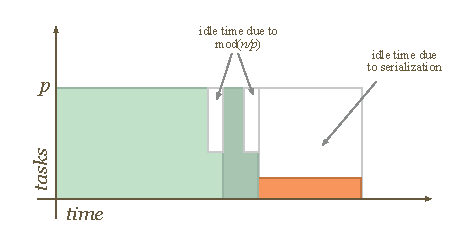
\includegraphics[scale=1.0]{figures/reduction-load-imbalance.pdf}
    \end{figure}
%
  \item excessive coarsening tends to increase load imbalance
  \item so can inappropriate mapping
  \item synchronization also causes load imbalance (see later slide)
  \item new upper bound for the speedup
    \[
    \sigma \leq \frac{w_{1}}{{\rm max}_{p}(w_{p} + {\rm idle})}
    \]
      
  \end{itemize}
%
\end{frame}

% --------------------------------------
% overhead
\begin{frame}[fragile]
%
  \frametitle{Parallelization overhead}
%
  \begin{itemize}
%
  \item there is always some extra work that is not present in the sequential implementation
    \begin{figure}
      \centering
      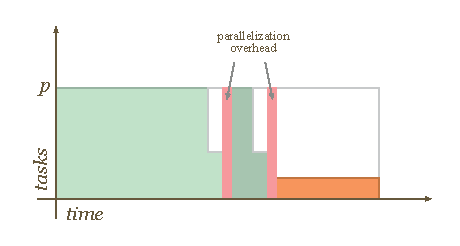
\includegraphics[scale=1.0]{figures/reduction-overhead.pdf}
    \end{figure}
%
  \item orchestration, management, bookkeeping
    \[
    \sigma \leq \frac{w_{1}}{{\rm max}_{p}(w_{p} + {\rm idle} + {\rm overhead})}
    \]
      
%
  \end{itemize}
%
\end{frame}

% --------------------------------------
% communication and synchronization costs
\begin{frame}[fragile]
%
  \frametitle{Communication and synchronization costs}
%
  \begin{itemize}
%
  \item communication is required for data movement and synchronization
    \begin{figure}
      \centering
      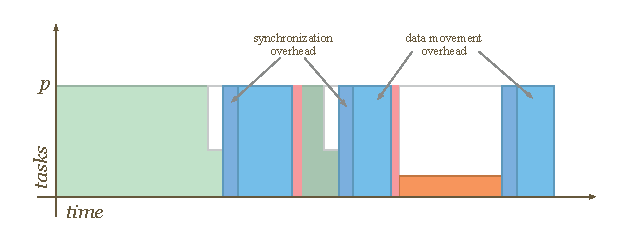
\includegraphics[scale=0.75]{figures/reduction-comsync.pdf}
    \end{figure}
%
  \item the cost is modeled by
    \[
    T_{c} = \lambda + \beta L
    \]
    where the {\em latency} $\lambda$ measures the communication startup cost, $\beta$ is the
    bandwidth of the interconnect and $L$ is the message length in {\em words} 
%
  \item the speedup is now bounded by
    \[
    \sigma \leq \frac{w_{1}}{{\rm max}_{p}(w_{p} + {\rm idle} + {\rm overhead} + {\rm comm})}
    \]
%      
  \end{itemize}
%
\end{frame}

% --------------------------------------
% reducing communication costs
\begin{frame}[fragile]
%
  \frametitle{Reducing communication costs}
%
  \begin{itemize}
%
  \item multiple strategies
%
  \item co\"ordinating placement of work and the associated data to minimize inter-process
    dependencies
    \begin{figure}
      \centering
      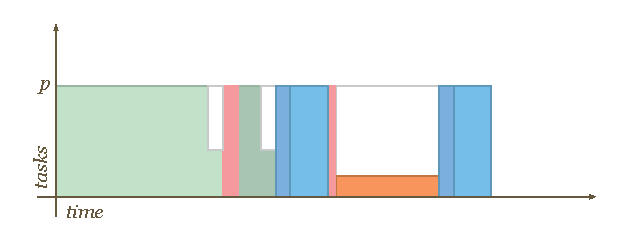
\includegraphics[scale=0.5]{figures/reduction-comsync-replication.pdf}
    \end{figure}
%
  \item trading memory for efficiency by replicating data
%
  \item trading cpu for efficiency by doing redundant work
    \begin{figure}
      \centering
      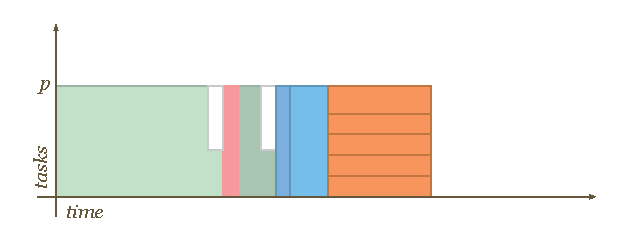
\includegraphics[scale=0.5]{figures/reduction-comsync-redundancy.pdf}
    \end{figure}
%
  \item improving communication efficiency by tuning the cost factors
    \begin{itemize}
    \item communication frequency, message size, contention, architecture specific
      optimizations
    \end{itemize}
%
  \end{itemize}
%
\end{frame}

% --------------------------------------
% tension
\begin{frame}[fragile]
%
  \frametitle{Optimizing speedup and efficiency}
  \begin{itemize}
%
    \item the goal is to minimize the denominator
      \[
      \sigma \leq \frac{w_{1}}{{\rm max}_{p}(w_{p} + {\rm idle} + {\rm overhead} + {\rm comm})}
      \]
      \begin{itemize}
        \item but its parts are in tension: minimizing one happens at the expense of another
      \end{itemize}
%
  \item fine grain decomposition and intelligent mapping tend to minimize load imbalance at the
    cost of increased communication
    \begin{itemize}
    \item coarser grains imply larger message size and fewer synchronization events
    \item for many problems communication costs decrease as surface to volume
    \end{itemize}
%
  \item na\"ive static partitioning reduces redundant work but cause load imbalance
%
  \end{itemize}
%
\end{frame}

% --------------------------------------
% the good news
\begin{frame}[fragile]
%
  \frametitle{The good news}
%
  \begin{itemize}
%
  \item the basic work unit of a parallel algorithm may be more efficient (and better
    performing) than the sequential equivalent
    \begin{itemize}
    \item only a small fraction of typical problems fits in L2 cache
    \item single node performance {\em requires} partitioning
    \item just like the parallel implementation
    \item don't be surprised by the poor quality of your sequential version after you see
      your parallel implementation
    \end{itemize}
%
  \item communication can be interleaved with computation
    \begin{itemize}
    \item better algorithms on today's complicated memory hierarchies
    \end{itemize}
%
    \item parallel algorithms may lead to better sequential ones
      \begin{itemize}
        \item e.g.~parallel search may explore configuration space more effectively
      \end{itemize}
%
  \end{itemize}
%
\end{frame}

% end of file 

%% -*- LaTeX -*-
% -*- coding: utf-8 -*-
%
% michael a.g. aïvázis
% california institute of technology
% (c) 1998-2012 all rights reserved
%

\lecture{Programming with pthreads - part 2}{20120125}

% --------------------------------------
% hello world
\begin{frame}[fragile]
%
  \frametitle{Hello world}
  \label{slide:hello-world-threads}
%
  \begin{C}
#include <pthread.h>
#include <stdio.h>
#define THREADS 10

void* hello(void* threadID) {
    long id = (long) threadID;
    printf("hello from %02ld/%0d\n", id, THREADS);
    pthread_exit(NULL);
    return NULL;
}

int main(int argc, char* argv[]) {
    long id;
    int status;
    pthread_t threads[THREADS];

    for (id=0; id<THREADS; id++) {
        printf("creating thread %02ld\n", id);
        status = pthread_create(&threads[id], NULL, hello, (void*) id);
        if (status) {
            printf("error %d in pthread_create\n", status);
        }
    }
    /* there is a problem here... */
    pthread_exit(NULL);
    return 0;
}
  \end{C}
%
\end{frame}

% --------------------------------------
% joining and detaching threads
\begin{frame}[fragile]
%
  \frametitle{Joining and detaching}
%
  \begin{itemize}
%
  \item in the example in \slideref{hello-world-threads}, the main thread exits without knowing whether
    any of the threads it spawned have finished
    \begin{itemize}
    \item saying ``hello'' is asynchronous
    \item but gathering the results of parallel calculations normally isn't
    \end{itemize}
%
  \item {\em thread synchronization} can be achieved using \function{pthread\_join}
    \begin{itemize}
      \item the \function{pthread\_create} caller saves the thread id
      \item the thread is scheduled, executes, and calls \function{pthread\_exit}
      \item any other thread can wait for this thread to finish by calling
        \function{pthread\_join} with the saved thread id and also retrieve the termination
        status
    \end{itemize}
%
  \item for this to work, a thread must be {\em joinable}
    \begin{itemize}
    \item controlled by the thread creation attributes
    \item for portability, you should always mark your joinable threads explicitly
    \end{itemize}
%
%
    \item a thread that will never be joined may be {\em detached}
      \begin{itemize}
      \item by setting the corresponding attribute during thread creation
      \item or, by calling \function{pthread\_detach} at any point
      \item detaching a thread saves some system resources
      \end{itemize}
        
  \end{itemize}
%
\end{frame}

% --------------------------------------
% mutexes
\begin{frame}[fragile]
%
  \frametitle{Creating mutexes}
%
  \begin{itemize}
%
  \item a {\em mutex} is a locking mechanism that helps guarantee exclusive access to a section
    of code, most often to control access to shared variables
%
  \item mutexes are created using
%
    \begin{C}
int pthread_mutex_init(
    pthread_mutex_t* mutex, const pthread_mutexattr_t* attr);
    \end{C}
%
    \begin{itemize}
    \item they start out unlocked
    \item the \identifier{attr} enables more advanced (but perhaps non-portable) use
    \end{itemize}
%
  \item mutexes are destroyed using
%
    \begin{C}
int pthread_mutex_destroy(pthread_mutex_t* mutex);
    \end{C}
%
    \begin{itemize}
    \item destroy mutexes you are no longer using to prevent resource leakage
    \end{itemize}
%
  \end{itemize}
%
\end{frame}

% --------------------------------------
% mutex manipulation
\begin{frame}[fragile]
%
  \frametitle{Locking and unlocking mutexes}
%
  \begin{itemize}
%
  \item threads manipulate mutexes through
%
    \begin{C}
int pthread_mutex_lock(pthread_mutex_t* mutex);
int pthread_mutex_trylock(pthread_mutex_t* mutex);
int pthread_mutex_unlock(pthread_mutex_t* mutex);
    \end{C}
%
  \item \identifier{pthread\_mutex\_lock} attempts to gain exclusive access
    \begin{itemize}
    \item if the mutex is unlocked, it locks it and returns
    \item otherwise, it blocks until the mutex is unlocked; when the mutex is unlocked, it
      locks it and returns
    \end{itemize}
%
  \item \identifier{pthread\_mutex\_unlock} attempts to release a mutex
    \begin{itemize}
    \item if it was previously locked by this thread, the mutex is unlocked
    \item if it was not previously locked, the call returns with an error code
    \item if it was locked, but not by the calling thread, the call returns an error code
    \end{itemize}
%
  \item \identifier{pthread\_mutex\_trylock} attempts to lock the mutex
    \begin{itemize}
    \item if it is unlocked, the call locks it and returns
    \item if it is locked, the call returns immediately with a {\em busy} error code
    \end{itemize}
%
  \item locking and unlocking mutexes is explicitly orchestrated by the programmer
  \item when multiple threads are blocked waiting for a mutex, there is no way to predict which
    one will succeed when the mutex becomes available
%
  \end{itemize}
%
\end{frame}


% --------------------------------------
% reduction using shared memory
\begin{frame}[fragile]
%
  \frametitle{Reduction on a shared memory machine}
%
%
  \begin{figure}
    \centering
    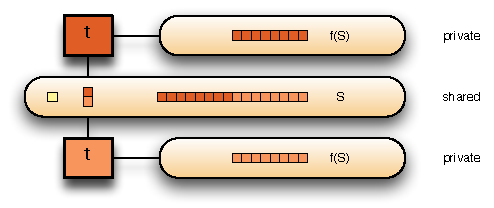
\includegraphics[width=\linewidth]{figures/threads-reduction.pdf}
    \label{fig:reduction-shared}
  \end{figure}
%
\end{frame}

% --------------------------------------
% sum of squares
\begin{frame}[fragile]
%
  \frametitle{Example reduction using threads}
  \label{slide:squares-threads}
%
  \begin{C}[basicstyle=\tt\bfseries\tiny]
#include <pthread.h>
#include <stdio.h>
#define THREADS 10
/* global variables -- yuck! */
long sum = 0;
pthread_mutex_t mutex;
/* worker */
void* squares(void* threadID) {
    long id = (long) threadID;
    pthread_mutex_lock(&mutex);
    sum += id*id;
    pthread_mutex_unlock(&mutex);
    pthread_exit(NULL);
    return NULL;
}
/* main program */
int main(int argc, char* argv[]) {
    long id;
    pthread_t threads[THREADS];
    pthread_mutex_init(&mutex, NULL);
    /* create some threads */
    for (id=0; id<THREADS; id++) {
        pthread_create(&threads[id], NULL, squares, (void*) id);
    }
    /* wait for them  to finish */
    for (id=0; id<THREADS; id++) {
        pthread_join(threads[id], NULL);
    }
    /* print the result */
    printf("sum = %ld\n", sum);
    /* exit */
    pthread_exit(NULL);
    return 0;
}
  \end{C}
%
\end{frame}

% --------------------------------------
% condition variables
\begin{frame}[fragile]
%
  \frametitle{Condition variables}
%
  \begin{itemize}
%
  \item condition variables build upon mutexes to enable threads to signal each other when some
    condition is met
%
  \item they are created using
%
    \begin{C}
int pthread_cond_init(
    pthread_cond_t* condition, const pthread_condattr_t* attr);
    \end{C}
%
  \item and destroyed using
%
    \begin{C}
int pthread_cond_destroy(pthread_cond_t* condition);
    \end{C}
%
  \end{itemize}
%
\end{frame}

% --------------------------------------
% using condition variables
\begin{frame}[fragile]
%
  \frametitle{Using condition variables}
%
  \begin{itemize}
%
  \item the following three routines implement the condition variable semantics
%
    \begin{C}
int pthread_cond_wait(pthread_cond_t* cond, pthread_mutex_t* mutex);
int pthread_cond_signal(pthread_cond_t* cond);
int pthread_cond_broadcast(pthread_cond_t* cond);
    \end{C}
%
  \item \identifier{pthread\_cond\_wait} blocks the calling thread until the specified
    condition is {\em signaled}
    \begin{itemize}
    \item it must be called with the mutex locked by the calling thread
    \item \identifier{pthread\_cond\_wait} releases the lock while the thread is blocked
    \item after the matching signal is received, the thread is awakened and the mutex locked
    \item the thread is responsible for releasing the mutex when it is done
    \end{itemize}
%
  \item \identifier{pthread\_cond\_signal} wakes up a thread that is waiting for the given
    condition variable
    \begin{itemize}
    \item mutex must be locked before calling it
    \item mutex must be unlocked after signaling, so blocking threads can be awakened
    \end{itemize}
%
  \item \identifier{pthread\_cond\_broadcast} can be used instead if multiple threads are
    waiting for a signal
%
  \end{itemize}
%
\end{frame}

% --------------------------------------
% condition variable caveats
\begin{frame}[fragile]
%
  \frametitle{Condition variable caveats}
%
  \begin{itemize}
%
  \item be careful with condition variables; make sure that
    \begin{itemize}
    \item a thread has called \identifier{pthread\_cond\_wait} before any thread
      calls \identifier{pthread\_cond\_signal}
    \item the mutex associated with the condition is locked before calling
      \identifier{pthread\_cond\_wait}, otherwise it might {\em not block}
    \item the thread that calls \identifier{pthread\_cond\_signal} unlocks the associated
      mutex, otherwise the threads waiting for the signal will continue to block
    \end{itemize}
%
%
  \end{itemize}
%
\end{frame}

% --------------------------------------
% the attribute interface
\begin{frame}[fragile]
%
  \frametitle{Attributes of threads, mutexes and condition variables}
%
  \begin{itemize}
%
  \item threads, mutexes and condition variables have associated attribute structures that can
    be used to tune the default creation parameters
%
  \item they are created and destroyed using
%
    \begin{C}
int pthread_attr_init(pthread_attr_t* attr);
int pthread_attr_destroy(pthread_attr_t* attr);

int pthread_mutexattr_init(pthread_mutexattr_t* attr);
int pthread_mutexattr_destroy(pthread_mutexattr_t* attr);

int pthread_condattr_init(pthread_condattr_t* attr);
int pthread_condattr_destroy(pthread_condattr_t* attr);
    \end{C}
%
  \item typically, the defaults are adequate and tuned to the details of the operating system
%
  \item if you make excessive use of the stack, e.g.~large arrays as local variable or deep
    recursion, you might want to know about
%
    \begin{C}
int pthread_attr_getstacksize(pthread_attr_t* attr, size_t* size);
int pthread_attr_setstacksize(pthread_attr_t* attr, size_t size);
    \end{C}
%
  \end{itemize}
%
\end{frame}

% --------------------------------------
% miscellaneous
\begin{frame}[fragile]
%
  \frametitle{Other useful routines}
%
  \begin{itemize}
%
  \item a thread can access its unique id assigned by the system by calling 
%
    \begin{C}
pthread_t pthread_self(void);
    \end{C}
%
  \item since system thread ids are opaque types, you cannot use \operator{==} to compare
    them; instead, use
%
    \begin{C}
int pthread_equal(pthread_t id1, pthread_t id2);
    \end{C}
%
  \item you can place all thread initialization code in a startup routine and call
%
    \begin{C}
int pthread_once(pthread_once_t* control_structure, void (*startup_routine)(void));
    \end{C}
%
  \end{itemize}
%
\end{frame}

% --------------------------------------
% template
\begin{frame}[fragile]
%
  \frametitle{Advanced topics}
%
  \begin{itemize}
%
  \item there is quite a bit more in the standard
%
  \item {\em keys}: creating and accessing per-thread data
    \begin{itemize}
    \item as the code get more complicated, it becomes increasingly difficult to pass complete
      thread-specific information from function to function
    \item possible solutions:
      \begin{itemize}
      \item the \fortran\ syndrome, where subroutines end up having dozens of arguments
      \item global variables
      \item an associative container that allows each thread to store and retrieve arbitrary
        data
      \end{itemize}
%
    \end{itemize}
%
    \item finer control over thread scheduling
      \begin{itemize}
      \item scheduling algorithms and priorities are implementation dependent
      \item there are routines in the standard that enable explicit tuning
      \item the standard guarantees that the routines will be {\em available}, but they don't
        have to be {\em implemented}
      \end{itemize}
%
    \item condition variable sharing across processes
%
    \item explicitly canceling threads
%
    \item the somewhat complicated interactions between threads and signals
%
    \item other synchronization constructs: barriers and read/write locks
%
  \end{itemize}
%
\end{frame}

% --------------------------------------
% summary
\begin{frame}[fragile]
%
  \frametitle{Summary}
%
  \begin{itemize}
%
  \item well-designed threaded programs must follow the same strategy as any other concurrent
    program
    \begin{figure}
      \centering
      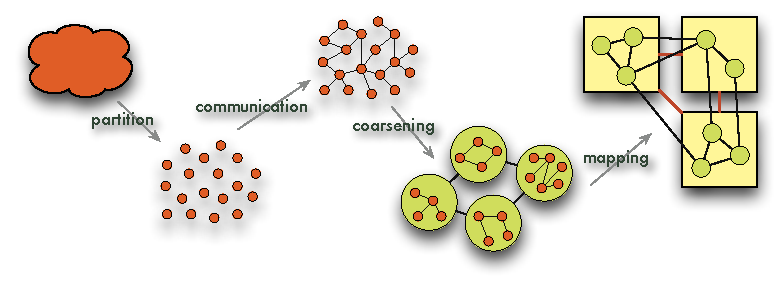
\includegraphics[scale=0.5]{figures/parallelization-steps.pdf}
      \label{fig:parallelization-steps-threads}
    \end{figure}
    \vspace{-1.75em}
%
    \begin{itemize}
    \item identify the work that can be done concurrently
    \item partition it in terms of work units, the fine grain tasks
    \item analyze the communication patterns among work units with an eye for critical sections
      and protecting shared data structures
    \item coarsen into threads, define the mutex categories and synchronization points
    \item let the OS schedule the threads onto physical processors
    \end{itemize}
%
  \item debugging threaded programs is very difficult
    \begin{itemize}
    \item preventing bugs through careful design is critical
    \item so is instrumenting the program to gain confidence in its execution
    \end{itemize}
%
  \end{itemize}
%
\end{frame}

% end of file 

%% -*- LaTeX -*-
% -*- coding: utf-8 -*-
%
% michael a.g. aïvázis
% california institute of technology
% (c) 1998-2012 all rights reserved
%

\lecture{Programming with MPI}{20120127}

% --------------------------------------
% template
\begin{frame}[fragile]
%
  \frametitle{Distributed memory parallelism}
%
  \begin{itemize}
%
  \item recall the generic layout of a distributed memory machine
%
    \begin{figure}
      \centering
      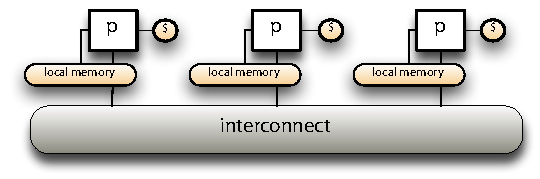
\includegraphics[scale=1.0]{figures/distributed-memory.pdf}
    \end{figure}
    \vspace{-1.0em}
%
    \begin{itemize}
      \item each processor has its own private memory space
      \item processors communicate via the interconnect substrate
    \end{itemize}
%
  \item the programming model
    \begin{itemize}
    \item program consists of a collection of $p$ named processes
      \item each process has its own instruction stream and address space
    \item logically shared data must be partitioned among the processors
    \item communication and synchronization must be orchestrated explicitly 
    \item processes communicate via explicit data exchanges
    \end{itemize}
%
  \end{itemize}
%
\end{frame}

% --------------------------------------
% template
\begin{frame}[fragile]
%
  \frametitle{\mpi\ -- the survivor}
%
  \begin{itemize}
%
  \item the {\em de facto} standard for writing parallel programs using message passing
    \begin{itemize}
    \item a library of routines callable from almost any programming language
    \item that enables communication among multiple processes
    \item standardized and portable API with good implementations available for almost any kind
      of parallel computer
    \end{itemize}
%
  \item \mpi\ is large and complex
    \begin{itemize}
    \item more than 125 functions, lot's of options and communication protocols
    \item but for most practical purposes, a small subset will suffice
    \item short introduction today, more when we consider specific physics
    \end{itemize}
%
  \item two major versions available -- check your installation for compliance
    \begin{itemize}
    \item \mpi-1: parallel machine management, process groups, collective operations,
      point-to-point operations, virtual topologies, profiling
    \item \mpi-2: dynamic process management, one-sided operations, parallel I/O, (simplistic)
      bindings for \cpp
    \end{itemize}
%
  \item \identifier{openmpi}: currently the best open source implementation
    \begin{itemize}
    \item well-architected, thread safe, fast, decent support from a broad community
    \end{itemize}
  \end{itemize}
%
\end{frame}

% --------------------------------------
% compiling, linking, staging and launching
\begin{frame}[fragile]
%
  \frametitle{Getting started}
%
  \begin{itemize}
%
  \item compiling and linking:
    \begin{itemize}
    \item most \mpi\ implementation supply wrappers around the available compilers
      \begin{itemize}
      \item e.g.~\identifier{mpicc}, \identifier{mpic++}, \identifier{mpif77},
        \identifier{mpif90}
      \end{itemize}
    \item it's not magic, so you can do it on your own to
      \begin{itemize}
      \item override the system defaults (without upsetting the sysadmins...)
      \item build multiple versions so you can benchmark
      \end{itemize}
    \end{itemize}
%
  \item staging and launching:
    \begin{itemize}
    \item most implementations provide \identifier{mpirun} to
      \begin{itemize}
      \item control the total number of desired processes
      \item specify the hostnames of the machines to use
      \item specify the mapping of processes to machines/CPUs/cores
      \item establish the current working directory, if possible, for all processes
      \item launch the program
      \end{itemize}
%
    \item but most installations do not permit its use; they have queuing systems instead
      \begin{itemize}
      \item \identifier{PBS}, \identifier{LSF}, \identifier{torque}, \identifier{maui}, ...
      \item specified and documented in the ``welcome'' package of most supercomputer centers
      \item scheduling of jobs, guarantee exclusive access to your allocated machines,
        establish upper time limit, charge the right account for your uses
      \end{itemize}
    \end{itemize}
%
  \end{itemize}
%
\end{frame}

% --------------------------------------
% initializing the runtime environment
\begin{frame}[fragile]
%
  \frametitle{At runtime}
%
  \begin{itemize}
%
%
  \item initializing the co\"operating processes:
    \begin{C}
int MPI_Init(int* argc, char ***argv);
    \end{C}
    \begin{itemize}
    \item note the strange signature; see \slideref{hello-world-mpi} for an example of its use
    \item some implementations -- notably \identifier{MPICH}, the reference implementation --
      used command line arguments to pass information from \identifier{mpirun} to the runtime
      environment
    \item so they need {\em write} access to the command line arguments to strip the extras
    \item thankfully, not done any more
    \end{itemize}
%
  \item must be the first \mpi\ in your program; nothing is initialized correctly until it
    returns
    \begin{itemize}
    \item if this call does not return \identifier{MPI\_SUCCESS}, you should abort
    \end{itemize}
% 
  \item don't forget to shut everything down:
    \begin{C}
int MPI_Finalize(void);
    \end{C}
%
  \item must be the last \mpi\ call in your program; nothing is in usable state after it
    returns
%
  \end{itemize}
%
\end{frame}

% --------------------------------------
% communicators
\begin{frame}[fragile]
%
  \frametitle{Groups and communicators}
%
  \begin{itemize}
%
  \item every \mpi\ process belongs to at least one {\em group}
%
  \item groups have associated {\em communicators} that provide the context for data exchanges and
      synchronization among processes
%
  \item processes in a given communicator get {\em ranked}
    \begin{itemize}
    \item a communicator of $p$ processes assigns ranks 0 through $p-1$
    \item a process can discover the communicator size and its own rank by using
      \begin{C}
int MPI_Comm_size(MPI_Comm communicator, int* size);
int MPI_Comm_rank(MPI_Comm communicator, int* rank);
      \end{C}
    \end{itemize}
% 
  \item the \mpi\ runtime environment creates the {\em global} communicator
    \begin{itemize}
    \item known as \identifier{MPI\_COMM\_WORLD}
    \item all processes are members
    \end{itemize}
% 
  \item it is good practice to learn to manage your own
    \begin{itemize}
    \item to narrow down global operations to processor subsets
    \item to promote {\em reuse}
    \item more details later
    \end{itemize}
% 
  \end{itemize}
%
\end{frame}

% --------------------------------------
% hello world
\begin{frame}[fragile]
%
  \frametitle{Hello world}
%
  \label{slide:hello-world-mpi}
%
  \begin{C}
#include <mpi.h>
#include <stdio.h>

int main(int argc, char* argv[]) {
    int status;
    int rank, size;

    /* initialize MPI */
    status = MPI_Init(&argc, &argv);
    if (status != MPI_SUCCESS) {
        printf("error in MPI_Init; aborting...\n");
        return status;
    }

    /* all good -- get process info and display it */
    MPI_Comm_rank(MPI_COMM_WORLD, &rank);
    MPI_Comm_size(MPI_COMM_WORLD, &size);
    printf("hello from %03d/%03d!\n", rank, size);

    /* shut down MPI */
    MPI_Finalize();

    return 0;
}
  \end{C}
%
\end{frame}

% --------------------------------------
% messages
\begin{frame}[fragile]
%
  \frametitle{Messages}
%
  \begin{itemize}
%
  \item in general, data exchanges through MPI calls involve
    \begin{itemize}
    \item a communicator
      \begin{itemize}
      \item specifies which processes participate in the exchange
      \item resolves process ranks into processes
      \end{itemize}        
    \item {\em collective} operations involve the entire communicator
    \item {\em point-to-point} operations require the rank of the message source or destination
    \item the details of the message payload
      \begin{itemize}
      \item the address of the source buffer
      \item the data type of the buffer contents
      \item the number of items in the buffer
      \end{itemize}
    \end{itemize}
%
    \item \mpi\ provides some data abstractions to
      \begin{itemize}
      \item hide machine dependencies in the data representations to enhance portability and
        support heterogeneous clusters
      \item support user defined data types
      \item support non-contiguous data layouts
      \end{itemize}        
      
%
  \end{itemize}
%
\end{frame}

% --------------------------------------
% global operations
\begin{frame}[fragile]
%
  \frametitle{Collective operations: global reductions}
%
  \begin{itemize}
%
  \item {\em collective} operations involve all processes in a given communicator
%
  \item the \mpi\ version of our global reduction example uses
    \begin{C}
int MPI_Allreduce(
        void* send_buffer, void* recv_buffer,
        int count, MPI_Datatype datatype, MPI_Op operation,
        MPI_Comm communicator
        );
   \end{C}
%
  \item example legal values for \identifier{MPI\_Datatype}
    \begin{itemize}
    \item \cc: \identifier{MPI\_INT}, \identifier{MPI\_LONG}, \identifier{MPI\_DOUBLE} 
    \item \fortran: \identifier{MPI\_INTEGER}, \identifier{MPI\_DOUBLE\_PRECISION},
      \identifier{MPI\_COMPLEX}
    \end{itemize}
%
  \item legal values for \identifier{MPI\_Op}
    \begin{itemize}
    \item \identifier{MPI\_MAX}, \identifier{MPI\_MIN}, \identifier{MPI\_MAXLOC},
      \identifier{MPI\_MINLOC}
    \item \identifier{MPI\_SUM}, \identifier{MPI\_PROD}
    \item \identifier{MPI\_LAND}, \identifier{MPI\_LOR}, \identifier{MPI\_LXOR}
    \item \identifier{MPI\_BAND}, \identifier{MPI\_BOR}, \identifier{MPI\_BXOR}
    \item \identifier{MPI\_REPLACE}
    \end{itemize}
%
  \end{itemize}
%
\end{frame}

% --------------------------------------
% example reduction with mpi
\begin{frame}[fragile]
%
  \frametitle{Example reduction using \mpi}
%
  \label{slide:squares-mpi}
%
  \begin{C}[basicstyle=\tt\bfseries\tiny]
#include <mpi.h>
#include <stdio.h>

int main(int argc, char* argv[]) {
    int status;
    int rank;
    int square, sum;

    /* initialize MPI */
    status = MPI_Init(&argc, &argv);
    if (status != MPI_SUCCESS) {
        printf("error in MPI_Init; aborting...\n");
        return status;
    }

    /* get the process rank */
    MPI_Comm_rank(MPI_COMM_WORLD, &rank);
    /* form the square */
    square = rank*rank;
    /* each process contributes the square of its rank */
    MPI_Allreduce(&square, &sum, 1, MPI_INT,  MPI_SUM, MPI_COMM_WORLD);
    /* print out the result */
    printf("%03d: sum = %d\n", rank, sum);

    /* shut down MPI */
    MPI_Finalize();

    return 0;
}
  \end{C}
%
\end{frame}
% end of file 

%% -*- LaTeX -*-
% -*- coding: utf-8 -*-
%
% michael a.g. aïvázis
% california institute of technology
% (c) 1998-2012 all rights reserved
%

\lecture{More programming with MPI}{20120130}

% --------------------------------------
% messages
\begin{frame}[fragile]
%
  \frametitle{Messages}
%
  \begin{itemize}
%
  \item in general, data exchanges through MPI calls involve
    \begin{itemize}
    \item a communicator
      \begin{itemize}
      \item specifies which processes participate in the exchange
      \item resolves process ranks into processes
      \end{itemize}        
    \item {\em collective} operations involve the entire communicator
    \item {\em point-to-point} operations require the rank of the message source or destination
    \item the details of the message payload
      \begin{itemize}
      \item the address of the source buffer
      \item the data type of the buffer contents
      \item the number of items in the buffer
      \end{itemize}
    \end{itemize}
%
    \item \mpi\ provides some data abstractions to
      \begin{itemize}
      \item hide machine dependencies in the data representations to enhance portability and
        support heterogeneous clusters
      \item support user defined data types
      \item support non-contiguous data layouts
      \end{itemize}        
      
%
  \end{itemize}
%
\end{frame}

% --------------------------------------
% global operations
\begin{frame}[fragile]
%
  \frametitle{Collective operations: global reductions}
%
  \begin{itemize}
%
  \item {\em collective} operations involve all processes in a given communicator
%
  \item the \mpi\ version of our global reduction example uses
    \begin{C}
int MPI_Allreduce(
        void* send_buffer, void* recv_buffer,
        int count, MPI_Datatype datatype, MPI_Op operation,
        MPI_Comm communicator
        );
   \end{C}
%
  \item example legal values for \identifier{MPI\_Datatype}
    \begin{itemize}
    \item \cc: \identifier{MPI\_INT}, \identifier{MPI\_LONG}, \identifier{MPI\_DOUBLE} 
    \item \fortran: \identifier{MPI\_INTEGER}, \identifier{MPI\_DOUBLE\_PRECISION},
      \identifier{MPI\_COMPLEX}
    \end{itemize}
%
  \item legal values for \identifier{MPI\_Op}
    \begin{itemize}
    \item \identifier{MPI\_MAX}, \identifier{MPI\_MIN}, \identifier{MPI\_MAXLOC},
      \identifier{MPI\_MINLOC}
    \item \identifier{MPI\_SUM}, \identifier{MPI\_PROD}
    \item \identifier{MPI\_LAND}, \identifier{MPI\_LOR}, \identifier{MPI\_LXOR}
    \item \identifier{MPI\_BAND}, \identifier{MPI\_BOR}, \identifier{MPI\_BXOR}
    \item \identifier{MPI\_REPLACE}
    \end{itemize}
%
  \end{itemize}
%
\end{frame}

% --------------------------------------
% example reduction with mpi
\begin{frame}[fragile]
%
  \frametitle{Example reduction using \mpi}
%
  \label{slide:squares-mpi}
%
  \begin{C}[basicstyle=\tt\bfseries\tiny]
#include <mpi.h>
#include <stdio.h>

int main(int argc, char* argv[]) {
    int status;
    int rank;
    int square, sum;

    /* initialize MPI */
    status = MPI_Init(&argc, &argv);
    if (status != MPI_SUCCESS) {
        printf("error in MPI_Init; aborting...\n");
        return status;
    }

    /* get the process rank */
    MPI_Comm_rank(MPI_COMM_WORLD, &rank);
    /* form the square */
    square = rank*rank;
    /* each process contributes the square of its rank */
    MPI_Allreduce(&square, &sum, 1, MPI_INT,  MPI_SUM, MPI_COMM_WORLD);
    /* print out the result */
    printf("%03d: sum = %d\n", rank, sum);

    /* shut down MPI */
    MPI_Finalize();

    return 0;
}
  \end{C}
%
\end{frame}

% end of file 

%% -*- LaTeX -*-
% -*- coding: utf-8 -*-
%
% michael a.g. aïvázis
% california institute of technology
% (c) 1998-2012 all rights reserved
%

\lecture{Manipulating communicators and groups}{20120201}

% --------------------------------------
% sending and receiving messages
\begin{frame}[fragile]
%
  \frametitle{Point to point communication}
%
  \begin{itemize}
%
  \item to send a message
    \begin{C}
int MPI_Send(
        void* buffer, int count, MPI_Datatype datatype,
        int destination, int tag, MPI_Comm communicator
        );
   \end{C}
%
  \item to receive a message
    \begin{C}
int MPI_Recv(
        void* buffer, int count, MPI_Datatype datatype,
        int source, int tag, MPI_Comm communicator, MPI_Status* status
        );
   \end{C}
%
  \item the \identifier{tag} enables choosing the order you may receive pending messages
%
  \item but for a given (\identifier{source},\identifier{tag},\identifier{communicator})
    messages are received in the order they were sent
%
  \item receiving via wildcards: \identifier{MPI\_ANY\_SOURCE} and \identifier{MPI\_ANY\_TAG}
% 
  \item in {\em standard} communication mode, sending and receiving messages are {\em blocking},
   so the function does not return until you can safely access the \identifier{buffer}
   \begin{itemize}
   \item to read, free, etc.
   \end{itemize}
%
  \end{itemize}
%
\end{frame}

% --------------------------------------
% communication modes
\begin{frame}[fragile]
%
  \frametitle{Communication modes}
%
  \begin{itemize}
%
  \item in standard mode, the specification does not explicitly mention buffering strategy
    \begin{itemize}
    \item buffering messages would remove some of the access constraints but it requires time
      and storage for the multiple copies
    \item portability across implementations implies conservative assumptions about the order
      of initiation of sends and receives to avoid deadlock
    \end{itemize}
%
  \item in {\em ready} mode, you must post a receive before the matching send can be initiated
    \begin{itemize}
    \item \function{MPI\_Rsend}, \function{MPI\_Rrecv}
    \end{itemize}
%
  \item in {\em buffered} mode, sends can be initiated, and may complete, regardless of when
    the matching receive is initiate
    \begin{itemize}
    \item \function{MPI\_Bsend}, \function{MPI\_Brecv}
    \end{itemize}
%
  \item in {\em synchronous} mode, sends can be initiated regardless of whether the matching
    receive has been initiated, but the send will not return until the message has been
    received
    \begin{itemize}
    \item \function{MPI\_Ssend}, \function{MPI\_Srecv}
    \end{itemize}
  \end{itemize}
%
\end{frame}

% --------------------------------------
% asynchronous communications
\begin{frame}[fragile]
%
  \frametitle{Asynchronous communication}
%
  \begin{itemize}
%
  \item there are non-blocking versions of all these
    \begin{C}
int MPI_Isend(
        void* buffer, int count, MPI_Datatype datatype,
        int destination, int tag, 
        MPI_Comm communicator, MPI_Request* request
        );
    \end{C}
    \begin{itemize}
    \item faster, but you must take care to not access the message buffers until the messages
      have been delivered
    \item more details later in the course, as needed
    \end{itemize}
%
  \item for sends
    \begin{itemize}
    \item standard mode: \function{MPI\_Isend}
    \item ready mode: \function{MPI\_Irsend}
    \item buffered mode: \function{MPI\_Ibsend}
    \item synchronous mode: \function{MPI\_Issend}
    \end{itemize}
%
  \item only one call for receives: \function{MPI\_Irecv}
%
  \item extra \identifier{request} argument to check for completion of the request
    \begin{itemize}
    \item \function{MPI\_Test}, \function{MPI\_Wait} and their relatives
    \end{itemize}
%
  \end{itemize}
%
\end{frame}

% --------------------------------------
% creating communicators and groups
\begin{frame}[fragile]
%
  \frametitle{Creating communicators and groups}
%
  \begin{itemize}
%
  \item communicators and groups are intertwined  
    \begin{itemize}
    \item you cannot create a group without a communicator
    \item you cannot create a communicator without a group
    \end{itemize}
%
  \item the cycle is broken by \identifier{MPI\_COMM\_WORLD}
    \begin{C}[basicstyle=\tt\bfseries\tiny]
#include <mpi.h>

int main(int argc, char* argv[]) {
    /* declare a communicator and a couple of groups */
    int loner = 0;
    MPI_Comm workers;
    MPI_Group world_grp, workers_grp;

    /* initialize MPI; for brevity all status checks are omitted */
    MPI_Init(&argc, &argv);

    /* get the world communicator to build its group */
    MPI_Comm_group(MPI_COMM_WORLD, &world_grp);

    /* build another group by excluding a process */
    MPI_Group_excl(world_grp, 1, &loner, &workers_grp);

    /* now build a communicator out of the processes in workers_grp */
    MPI_Comm_create(MPI_COMM_WORLD, worker_grp, &workers);

    /* etc.... */

    /* shut down MPI */
    MPI_Finalize();

    return 0;
}
    \end{C}
%
  \end{itemize}
%
\end{frame}

% --------------------------------------
% freeing communicators and groups
\begin{frame}[fragile]
%
  \frametitle{Manipulating communicators and groups}
%
  \begin{itemize}
%
  \item releasing resources
    \begin{C}
int MPI_Group_free(MPI_Group* group);
int MPI_Comm_free(MPI_Comm* communicator);
int MPI_Comm_disconnect(MPI_Comm* communicator);
    \end{C}
%
  \item you can make a new group by adding or removing processes from an existing one
    \begin{C}
int MPI_Group_incl(
    MPI_Group grp, int n, int* ranks, MPI_Group* new_group);
int MPI_Group_excl(
    MPI_Group grp, int n, int* ranks, MPI_Group* new_group);
    \end{C}
%
  \item or by using set operations
    \begin{C}
int MPI_Group_union(
    MPI_Group grp1, MPI_Group grp2, MPI_Group* new_group);
int MPI_Group_intersection(
    MPI_Group grp1, MPI_Group grp2, MPI_Group* new_group);
int MPI_Group_difference(
    MPI_Group grp1, MPI_Group grp2, MPI_Group* new_group);
    \end{C}
%
  \end{itemize}
%
\end{frame}

% end of file

%% -*- LaTeX -*-
% -*- coding: utf-8 -*-
%
% michael a.g. aïvázis
% california institute of technology
% (c) 1998-2012 all rights reserved
%

\lecture{Data movement with MPI}{20120203}


% --------------------------------------
% timing
\begin{frame}[fragile]
%
  \frametitle{Timing}
%
  \begin{itemize}
%
  \item the function
    \begin{C}
double MPI_Wtime();
    \end{C}
    returns the time in seconds from some arbitrary time in the past
    \begin{itemize}
    \item guaranteed not to change only for the duration of the process
    \end{itemize}
%
  \item you can compute the elapsed time for any program segment by making calls at the
    beginning and the end and computing the difference
%
  \item no guarantees about synchronized clocks among different processes
%
  \item you can compute the clock resolution by using
    \begin{C}
double MPI_Wtick();
    \end{C}
%
  \end{itemize}
%
\end{frame}

% --------------------------------------
% other collective operations
\begin{frame}[fragile]
%
  \frametitle{Other collective operations}
%
  \begin{itemize}
%
  \item \function{MPI\_Scan} computes partial reductions: the \th{p} process receives the
    result from processes 0 through $p-1$
    \begin{C}
int MPI_Scan(
        void* send_buffer, void* recv_buffer,
        int count, MPI_Datatype datatype, MPI_Op operation,
        MPI_Comm communicator
        );
   \end{C}
%
  \item \function{MPI\_Reduce} collects the result at only the given process \identifier{root}
    \begin{C}
int MPI_Reduce(
        void* send_buffer, void* recv_buffer,
        int count, MPI_Datatype datatype, MPI_Op operation,
        int root, MPI_Comm communicator
        );
   \end{C}
%
   \item synchronization is also a global operation:
    \begin{C}
int MPI_Barrier(MPI_Comm communicator);
   \end{C}
%
   participating processes block at a barrier until they have all reached it
%
  \end{itemize}
%
\end{frame}

% --------------------------------------
% scatter
\begin{frame}[fragile]
%
  \frametitle{Scatter}
%
  \begin{itemize}
%
  \item \function{MPI\_Scatter} sends data from \identifier{root} to all processes 
    \begin{C}
int MPI_Scatter(
        void* send_buffer, int send_count, MPI_Datatype send_datatype,
        void* recv_buffer, int recv_count, MPI_Datatype recv_datatype,
        int root, MPI_Comm communicator
        );
    \end{C}
    \begin{figure}
      \centering
      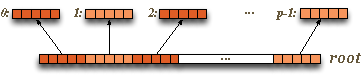
\includegraphics[scale=1.0]{figures/mpi-scatter.pdf}
    \end{figure}
%
  \item it is as if the data in \identifier{send\_buffer} were split in $p$ segments, and the
    \th{i} process receives the \th{i} segment
%
  \item the \identifier{send\_xxx} arguments are only meaningful for \identifier{root}; they
    are ignored for other processes
%
  \item the arguments \identifier{root} and \identifier{communicator} must be passed identical
    values by all processes
%
  \end{itemize}
% 
\end{frame}

% --------------------------------------
% gather
\begin{frame}[fragile]
%
  \frametitle{Gather}
%
  \begin{itemize}
%
  \item the converse is \function{MPI\_Gather} with \identifier{root} receiving data from all
    processes
    \begin{C}
int MPI_Gather(
        void* send_buffer, int send_count, MPI_Datatype send_datatype,
        void* recv_buffer, int recv_count, MPI_Datatype recv_datatype,
        int root, MPI_Comm communicator
        );
   \end{C}
   \begin{figure}
     \centering
     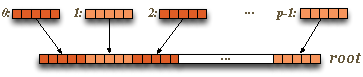
\includegraphics[scale=1.0]{figures/mpi-gather.pdf}
   \end{figure}
%
  \item it is as if $p$ messages, one from each processes, were concatenated in rank order and
    placed at \identifier{recv\_buffer}
%
  \item the \identifier{recv\_xxx} arguments are only meaningful for \identifier{root}; they
    are ignored for other processes
%
  \item the arguments \identifier{root} and \identifier{communicator} must be passed identical
    values by all processes
%
  \end{itemize}
%
\end{frame}

% --------------------------------------
% broadcasts
\begin{frame}[fragile]
%
  \frametitle{Broadcasting operations}
%
  \begin{itemize}
%
  \item \function{MPI\_Alltoall} sends data from all processes to all processes in a global
    scatter/gather
    \begin{C}
int MPI_Alltoall(
        void* send_buffer, int send_count, MPI_Datatype send_datatype,
        void* recv_buffer, int recv_count, MPI_Datatype recv_datatype,
        MPI_Comm communicator
        );
   \end{C}
%
 \item use \function{MPI\_Bcast} to send the contents of a buffer from \identifier{root} to all
   processes in a communicator
   \begin{C}
int MPI_Bcast(
        void* buffer, int count, MPI_Datatype datatype,
        int root, MPI_Comm communicator
        );
   \end{C}
%
  \end{itemize}
%
\end{frame}

% --------------------------------------
% collective operations summary
\begin{frame}[fragile]
%
  \frametitle{Data movement patterns for the collective operations}
%
  \begin{tabular}{cc}
    \parbox[c][1in]{2in}{
      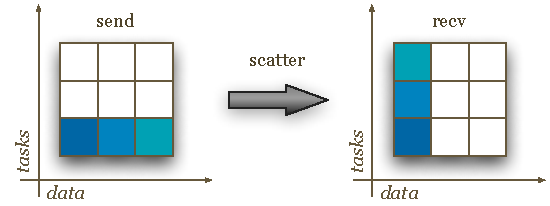
\includegraphics[scale=0.5]{figures/mpi-scatter-pattern.pdf}
    }
    &
    \parbox[c][1in]{2in}{
      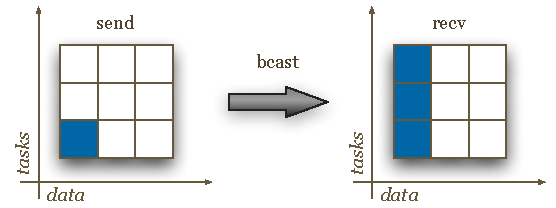
\includegraphics[scale=0.5]{figures/mpi-bcast-pattern.pdf}
    }
    \\ 
    \parbox[c][1in]{2in}{
      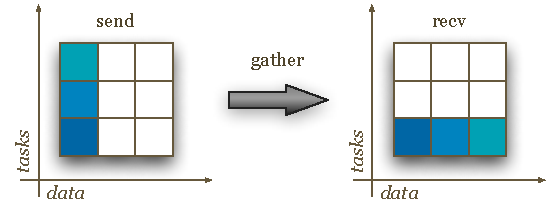
\includegraphics[scale=0.5]{figures/mpi-gather-pattern.pdf}
    }
    &
    \parbox[c][1in]{2in}{
      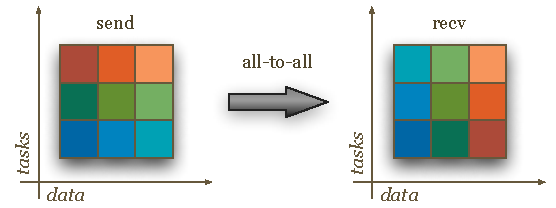
\includegraphics[scale=0.5]{figures/mpi-alltoall-pattern.pdf}
    }
  \end{tabular}
%
\end{frame}

% end of file

%% -*- LaTeX -*-
% -*- coding: utf-8 -*-
%
% michael a.g. aïvázis
% california institute of technology
% (c) 1998-2010  all rights reserved
%

\lecture{Three implementations of quadrature rule}{20100206}

% --------------------------------------
% problem statement
\begin{frame}[fragile]
%
  \frametitle{Approximating $\Li$ using a numerical quadrature}
%
  \begin{itemize}
%
  \item the second homework assignment involved $\Li(z)$, defined by
    \begin{equation*}
      \Li(z) \bydef - \int_{0}^{z} dz' \; \frac{\log(1-z')}{z'}
    \end{equation*}
%
    \item the assignment asked for approximating this integral using a simple
      quadrature based on the mid-point rule
      \begin{equation*}
      \Li(z) 
      \approx 
      \Li(z, N) 
      \bydef
      - \frac{z}{N} \sum_{n=0}^{N-1} \left.
        \frac{\log(1-z')}{z'}
      \right|_{z'=(n+\frac{1}{2})\frac{z}{N}}
    \end{equation*}
%
  \end{itemize}
%
\end{frame}

% --------------------------------------
% implementations
\begin{frame}[fragile]
%
  \frametitle{Quadrature rule}
%
  \begin{figure}
    \centering
    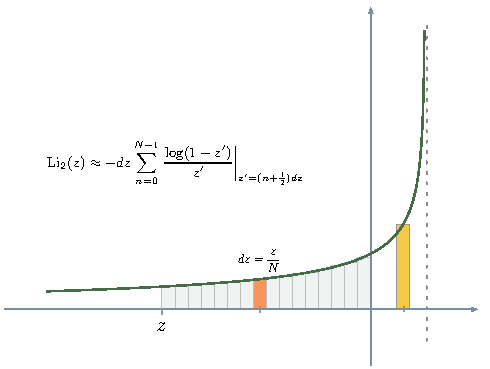
\includegraphics[width=0.9\linewidth]{figures/dilog-quadrature.pdf}
    \label{fig:reduction-shared}
  \end{figure}
%
\end{frame}

%
% --------------------------------------
% implementations
\begin{frame}[fragile]
%
  \frametitle{Implementations}
%
  \begin{itemize}
%
    \item three implementations
      \begin{itemize}
      \item sequential: to get a feeling for how to convert the algorithm into a functioning
        program
      \item parallel using threads: to walk through the parallelization steps and use
        \identifier{pthreads} to get better performance
      \item parallel using \mpi: to get a feel for how \mpi-based programs solve the task
        partitioning problem
      \end{itemize}
%
    \item let's walk through composing, building and running
      \begin{itemize}
      \item on my desktop, and on \href{shc.cacr.caltech.edu}
      \end{itemize}
%
  \end{itemize}
%
\end{frame}

% --------------------------------------
% the sequential driver - preamble
\begin{frame}[fragile]
%
  \frametitle{Sequential implementation - part 1}
%
  \begin{itemize}
  \item the preamble
  \begin{lstlisting}[language=c++,name=sequential]
#include <getopt.h> // for getopt and friends
#include <cstdlib>  // for atof
#include <cmath>    // for the correct abs, log

#include <map>
#include <iostream>
#include <iomanip>
  \end{lstlisting}
%
  \item quadrature using the midpoint rule to avoid the singularities
  \begin{lstlisting}[language=c++,name=sequential]
// dilog
double dilog(double z, long N) {
    // initialize
    double dx = z/N;
    double x = dx/2;
    double sum = 0;
    // loop
    for (long i=0; i < N; i++) {
        sum += std::log(1-x)/x;
        x += dx;
    }
    // return; don't forget the sign
    return -dx * sum;
}

  \end{lstlisting}
%
  \end{itemize}
%
\end{frame}

% --------------------------------------
% the sequential driver - the main program
\begin{frame}[fragile]
%
  \frametitle{Sequential implementation - part 2}
%
  \begin{itemize}
  \item using the command line to set $z$ and the number of subdivisions $N$
  \begin{lstlisting}[language=c++,name=sequential]
// main program
int main(int argc, char* argv[]) {
    //  default values for the command line options
    long N = 1000;
    double z = 1.0;

    // read the command line
    int command;
    while ((command = getopt(argc, argv, "z:N:")) != -1) {
        switch (command) {
        // get the argument of the dilogarithm 
        case 'z':
            z = atof(optarg);
            break;
        // get the number of subdivisions
        case 'N':
            N = (long) atof(optarg);
            break;
        }
    }
  \end{lstlisting}
%
  \end{itemize}
%
\end{frame}

% --------------------------------------
% the sequential driver - the main program
\begin{frame}[fragile]
%
  \frametitle{Sequential implementation - part 3}
%
  \begin{itemize}
  \item error checking and computation of the numerical integral
  \begin{lstlisting}[language=c++,name=sequential]
    // error checking
    // abort if N < 1
    if (N < 1) {
        std::cout 
            << "the number of subdivisions must be positive"
            << std::endl;
        return 0;
    }

    // abort for z > 1 to avoid dealing with the imaginary part
    if (z > 1.0) {
        std::cout << "math domain error: z > 1" << std::endl;
        return 0;
    } 

    // compute
    double value = dilog(z, N);
  \end{lstlisting}
%
  \end{itemize}
%
\end{frame}

% --------------------------------------
% the sequential driver - the main program
\begin{frame}[fragile]
%
  \frametitle{Sequential implementation - part 4}
%
  \begin{itemize}
  \item computing the error and printing out the results
  \begin{lstlisting}[language=c++,name=sequential]
    // build a naive database of the known dilogarithm values
    const double pi = M_PI;
    std::map<double, double> answers;
    answers[1.0] = pi*pi/6;
    answers[-1.0] = -pi*pi/12;

    // print out the value
    std::cout << "Li2(" << z << ")="
        << std::setprecision(17) << std::endl
        << " computed: " << value << std::endl;
    // check whether we know the right answer
    std::map<double,double>::const_iterator lookup = answers.find(z);
    if (lookup != answers.end()) {
        // and if we do, print it out
        double exact = lookup->second;
        std::cout << "    exact: " << exact << std::endl;
        // compute the approximation error and print it out
        double error = std::abs(exact-value)/exact;
        std::cout 
            << std::setiosflags(std::ios_base::scientific) 
            << "    error: " << error << std::endl;
    }

    return 0;
}
  \end{lstlisting}
%
  \end{itemize}
%
\end{frame}

% --------------------------------------
% running the sequential driver
\begin{frame}[fragile]
%
  \frametitle{Building and running the sequential driver}
%
  \begin{shell}{}
#> g++ dilog-quadrature_sequential
#> dilog-sequential -N 1e9 -z 1.0
Li2(1)=
 computed: 1.6449339414016682
    exact: 1.6449340668482264
    error: 7.62623625958871898e-08

real    0m19.885s
user    0m19.877s
sys     0m0.003s
#>
  \end{shell}
%
\end{frame}

% --------------------------------------
% the threaded driver - preamble
\begin{frame}[fragile]
%
  \frametitle{Threaded implementation - part 1}
%
  \begin{itemize}
  \item the preamble
  \begin{lstlisting}[language=c++,name=threaded]
#include <getopt.h> // for getopt and friends
#include <pthread.h>

#include <cstdio>
#include <cstdlib>  // for atof
#include <cmath>

#include <map>
#include <iostream>
#include <iomanip>

  \end{lstlisting}
%
  \end{itemize}
%
\end{frame}

% --------------------------------------
% the threaded driver - thread data structures
\begin{frame}[fragile]
%
  \frametitle{Threaded implementation - part 2}
%
  \begin{itemize}
  \item private and shared data structures
  \begin{lstlisting}[language=c++,name=threaded]
// shared information
struct problem {
    int workers;           // total number of threads
    double dz;             // the width of each subdivision
    double sum;            // storage for the partial computations

    pthread_mutex_t lock;  // mutex to control access to the sum
};

// thread specific information
struct context {
    // thread info
    int id;
    pthread_t descriptor;
    // the workload for this thread
    long subdivisions;  // number of subdivisions
    double z_low;       // the lower limit of integration
    double partial;     // record the partial sum computed by this thread
    // the shared problem information
    problem* info;
};
  \end{lstlisting}
%
  \end{itemize}
%
\end{frame}

% --------------------------------------
% the threaded driver - worker
\begin{frame}[fragile]
%
  \frametitle{Threaded implementation - part 3}
%
  \begin{itemize}
  \item the coarse grain task
  \begin{lstlisting}[language=c++,name=threaded]
// worker
void* worker(void* arg) {
    context* ctxt = (context *) arg;
    // pull the problem information from the thread context
    double dz = ctxt->info->dz;
    double z = ctxt->z_low + dz/2;
    // loop over the subdivisions assigned to this thread
    double sum = 0.0;
    for (long i=0; i < ctxt->subdivisions; i++) {
        sum += std::log(1-z)/z;
        z += dz;
    }
    // multiply by the width of each subdivision and adjust the sign
    sum *= -dz;

    // grab the lock
    pthread_mutex_lock(&(ctxt->info->lock));
    // store the result
    ctxt->info->sum += sum;
    // and release the lock
    pthread_mutex_unlock(&(ctxt->info->lock));

    // all done
    return 0;
}
  \end{lstlisting}
%
  \end{itemize}
%
\end{frame}

% --------------------------------------
% the threaded driver - task master
\begin{frame}[fragile]
%
  \frametitle{Threaded implementation - part 4}
%
  \begin{itemize}
  \item the task master -- interface and allocation of storage
  \begin{lstlisting}[language=c++,name=threaded]
// driver
double dilog(double z, long N, int threads) {
    // the width of each interval subdivision
    const double dz = z/N;

    // setup the problem context
    problem info;
    info.workers = threads;
    info.dz = dz;
    info.sum = 0.0;
    pthread_mutex_init(&info.lock, 0);

    // and an array to hold the thread contexts
    context thr_info[threads];
    // partition the number of subdivisions
    long nominal_load = N/threads;
  \end{lstlisting}
%
  \end{itemize}
%
\end{frame}

% --------------------------------------
% the threaded driver - task master continued
\begin{frame}[fragile]
%
  \frametitle{Threaded implementation - part 5}
%
  \begin{itemize}
  \item the task master -- spawning the threads
  \begin{lstlisting}[language=c++,name=threaded]
    // spawn the workers
    for (int tid=0; tid<threads; tid++) {
        // store the thread id
        thr_info[tid].id = tid;
        // point to the shared problem info
        thr_info[tid].info = &info;

        // compute the starting point of the partial integral
        thr_info[tid].z_low = tid*nominal_load*dz;
        // compute the number of subdivisions for this thread
        if (tid == threads - 1) {
            // the last thread gets the leftovers
            thr_info[tid].subdivisions = N - tid*nominal_load;
        } else {
            thr_info[tid].subdivisions = nominal_load;
        }

        // create the thread
        int status = pthread_create(
            &(thr_info[tid].descriptor), 0, worker, &thr_info[tid]);
        if (status) {
            printf("error %d in pthread_create\n", status);
        }
    }
  \end{lstlisting}
%
  \end{itemize}
%
\end{frame}

% --------------------------------------
% the threaded driver - task master continued
\begin{frame}[fragile]
%
  \frametitle{Threaded implementation - part 6}
%
  \begin{itemize}
  \item the task master -- harvesting the threads and returning the result
  \begin{lstlisting}[language=c++,name=threaded]
    // harvest the threads
    for (int tid=0; tid<threads; tid++) {
        pthread_join(thr_info[tid].descriptor, 0);
    }

    // all done
    return info.sum;
}
  \end{lstlisting}
%
  \end{itemize}
%
\end{frame}

% --------------------------------------
% the threaded driver - main program
\begin{frame}[fragile]
%
  \frametitle{Threaded implementation - part 7}
%
  \begin{itemize}
  \item the main program -- reading the command line
  \begin{lstlisting}[language=c++,name=threaded]
// main program
int main(int argc, char* argv[]) {
    //  default values for the command line options
    long N = 1000;
    double z = 1.0;
    int threads = 8;

    // read the command line
    int command;
    while ((command = getopt(argc, argv, "z:N:t:")) != -1) {
        switch (command) {
        case 'z':
            // get the argument of the dilogarithm 
            z = atof(optarg);
            break;
        case 'N':
            // get the number of subdivisions
            N = (long) atof(optarg);
            break;
        case 't':
            // get the numberof threads
            threads = atoi(optarg);
            break;
        }
    }
  \end{lstlisting}
%
  \end{itemize}
%
\end{frame}

% --------------------------------------
% the threaded driver - main program
\begin{frame}[fragile]
%
  \frametitle{Threaded implementation - part 8}
%
  \begin{itemize}
  \item error checking and the invocation of the task master
  \begin{lstlisting}[language=c++,name=threaded]
    // error checking
    // abort if N < 1
    if (N < 1) {
        std::cout 
            << "the number of subdivisions must be positive"
            << std::endl;
        return 0;
    }

    // abort for z > 1 to avoid dealing with the imaginary part
    if (z > 1.0) {
        std::cout << "math domain error: z > 1" << std::endl;
        return 0;
    } 

    // compute
    double value = dilog(z, N, threads);
  \end{lstlisting}
%
  \end{itemize}
%
\end{frame}

% --------------------------------------
% the threaded driver - main program
\begin{frame}[fragile]
%
  \frametitle{Threaded implementation - part 9}
%
  \begin{itemize}
  \item the task master -- printing out the answers
  \begin{lstlisting}[language=c++,name=threaded]
    // build a database of the known dilogarithm values
    const double pi = M_PI;
    std::map<double, double> answers;
    answers[1.0] = pi*pi/6;
    answers[-1.0] = -pi*pi/12;

    // print out the value
    std::cout << "Li2(" << z << ")="
         << std::setprecision(17) << std::endl
         << " computed: " << value << std::endl;
    // check whether we know the right answer
    std::map<double,double>::const_iterator lookup = answers.find(z);
    if (lookup != answers.end()) {
        // and if we do, print it out
        double exact = lookup->second;
        std::cout << "    exact: " << exact << std::endl;
        // compute the approximation error and print it out
        double error = std::abs(exact-value)/exact;
        std::cout 
            << std::setiosflags(std::ios_base::scientific) 
            << "    error: " << error << std::endl;
    }

    return 0;
}
  \end{lstlisting}
%
  \end{itemize}
%
\end{frame}

% --------------------------------------
% running the threaded driver
\begin{frame}[fragile]
%
  \frametitle{Building and running the threaded driver}
%
  \begin{shell}{}
#> g++ dilog-threads.cc -o dilog-threads -pthread
#> dilog-threads -N 1e7 -z 1.0 -t 4
Li2(1)=
 computed: 1.6449340301295035
    exact: 1.6449340668482264
    error: 2.23223068274304058e-08
#> time dilog-threads -N 1e9 -z 1.0 -t 8
Li2(1)=
 computed: 1.6449340044883614
    exact: 1.6449340668482264
    error: 3.79102520315773892e-08

real    0m2.803s
user    0m20.693s
sys     0m0.006s
#>
  \end{shell}
%
\end{frame}

% --------------------------------------
% the mpi driver - the preamble
\begin{frame}[fragile]
%
  \frametitle{MPI implementation - part 1}
%
  \begin{itemize}
  \item the preamble
  \begin{lstlisting}[language=c++,name=mpi]
#include <getopt.h> // for getopt and friends
#include <mpi.h>

#include <cstdio>
#include <cstdlib>  // for atof
#include <cmath>

#include <map>
#include <iostream>
#include <iomanip>

  \end{lstlisting}
%
  \end{itemize}
%
\end{frame}

% --------------------------------------
% the mpi driver -  the coarse grain task
\begin{frame}[fragile]
%
  \frametitle{MPI implementation - part 2}
%
  \begin{itemize}
  \item coarse grain task
  \begin{lstlisting}[language=c++,name=mpi]
double dilog(double zprime, long N, int id, int processes) {
    // the width of each interval subdivision
    const double dz = zprime/N;
    // compute the starting point of the partial integral
    const double z_low = id*zprime/processes;
    // partition the number of subdivisions
    long nominal_load = N/processes;
    // the last process gets the leftovers
    if (id == processes - 1) {
        nominal_load = N - id*nominal_load;
    }
    // initialize the partial sum
    double sum = 0.0;
    double z = z_low + dz/2;
    // loop over the subdivisions assigned to this thread
    for (long i=0; i < nominal_load; i++)  {
        sum += std::log(1-z)/z;
        z += dz;
    }
    // collect the partial answers from all the processes
    double value;
    MPI_Allreduce(
        &sum, &value, 1, MPI_DOUBLE, MPI_SUM, MPI_COMM_WORLD);
    // multiply by the width of each subdivision and adjust the sign
    return -dz*value;
}
  \end{lstlisting}
%
  \end{itemize}
%
\end{frame}

% --------------------------------------
% the mpi driver - the main program
\begin{frame}[fragile]
%
  \frametitle{MPI implementation - part 3}
%
  \begin{itemize}
  \item the main program -- setting up \mpi
  \begin{lstlisting}[language=c++,name=mpi]
// main program
int main(int argc, char* argv[]) {
    // initialize MPI
    int status = MPI_Init(&argc, &argv);
    if (status != MPI_SUCCESS) {
        std::cout << "error in MPI_Init; aborting..." << std::endl;
        return status;
    }
    // get process information from the world communicator
    int id, processes;
    MPI_Comm_rank(MPI_COMM_WORLD, &id);
    MPI_Comm_size(MPI_COMM_WORLD, &processes);

  \end{lstlisting}
%
  \end{itemize}
%
\end{frame}

% --------------------------------------
% the mpi driver - the main program
\begin{frame}[fragile]
%
  \frametitle{MPI implementation - part 4}
%
  \begin{itemize}
  \item reading the command line
  \begin{lstlisting}[language=c++,name=mpi]
    //  default values for the command line options
    long N = 1000;
    double z = 1.0;
    // read the command line
    int command;
    while ((command = getopt(argc, argv, "z:N:")) != -1) {
        switch (command) {
        case 'z':
            // get the argument of the dilogarithm 
            z = atof(optarg);
            break;
        case 'N':
            // get the number of subdivisions
            N = (long) atof(optarg);
            break;
        }
    }
  \end{lstlisting}
%
  \end{itemize}
%
\end{frame}

% --------------------------------------
% the mpi driver -  error checking and computation
\begin{frame}[fragile]
%
  \frametitle{MPI implementation - part 5}
%
  \begin{itemize}
  \item error checking and computation
  \begin{lstlisting}[language=c++,name=mpi]
    // error checking
    // abort if N < 1
    if (N < 1) {
        if (id == 0) {
            std::cout 
                << "the number of subdivisions must be positive"
                << std::endl;
        }
        MPI_Finalize();
        return 0;
    }
    // abort for z > 1 to avoid dealing with the imaginary part
    if (z > 1.0) {
        if (id == 0) {
            std::cout << "math domain error: z > 1" << std::endl;
        }
        MPI_Finalize();
        return 0;
    } 
    // compute
    double value = dilog(z, N, id, processes);
    if (id != 0) { // let all but processor 0 die
        // shut down MPI
        MPI_Finalize();
        return 0;
    }
  \end{lstlisting}
%
  \end{itemize}
%
\end{frame}

% --------------------------------------
% the mpi driver - printing out the results
\begin{frame}[fragile]
%
  \frametitle{MPI implementation - part 6}
%
  \begin{itemize}
  \item printing out the results
  \begin{lstlisting}[language=c++,name=mpi]
    // build a database of the known dilogarithm values
    const double pi = M_PI;
    std::map<double, double> answers;
    answers[1.0] = pi*pi/6;
    answers[-1.0] = -pi*pi/12;

    // print out the value
    std::cout << "Li2(" << z << ")=" << std::setprecision(17) << std::endl;
    std::cout << " computed: " << value << std::endl;
    // check whether we know the right answer
    std::map<double,double>::const_iterator lookup = answers.find(z);
    if (lookup != answers.end()) {
        // and if we do, print it out
        double exact = lookup->second;
        std::cout << "    exact: " << exact << std::endl;
        // compute the approximation error and print it out
        double error = std::abs(exact-value)/exact;
        std::cout 
            << std::setiosflags(std::ios_base::scientific) 
            << "    error: " << error << std::endl;
    }

    // shut down MPI
    MPI_Finalize();
    return 0;
}
  \end{lstlisting}
%
  \end{itemize}
%
\end{frame}

% --------------------------------------
% running the mpi driver
\begin{frame}[fragile]
%
  \frametitle{Building and running the \mpi\ driver}
%
  \begin{itemize}
  \item on my desktop, or \href{mind-meld.cacr.caltech.edu}
    \begin{itemize}
    \item where there is no queue manager
    \end{itemize}
  \end{itemize}
%
  \begin{shell}{}
#> mpic++ dilog-mpi.cc -o dilog-mpi -lmpi_cxx -lmpi
#> mpirun -np 4 dilog-mpi -N 1e7 -z 1.0
Li2(1)=
 computed: 1.6449340301295035
    exact: 1.6449340668482264
    error: 2.23223068274304058e-08
#> time mpirun -np 8 dilog-mpi -N 1e9 -z 1.0
Li2(1)=
 computed: 1.6449340044883614
    exact: 1.6449340668482264
    error: 3.79102520315773892e-08

real    0m3.697s
user    0m0.018s
sys     0m0.015s
#>
  \end{shell}
%
\end{frame}

% --------------------------------------
% running the mpi driver
\begin{frame}[fragile]
%
  \frametitle{Running the \mpi\ driver on a shared resource}
%
  \begin{itemize}
  \item on \href{shc.cacr.caltech.edu} there is a queue manager
    \begin{itemize}
    \item don't use \identifier{mpirun}: you are running on the head node
    \item instead, request a dedicated node
    \end{itemize}
  \end{itemize}
%
  \begin{shell}{}
# shc-a> mpic++ dilog-mpi.cc -o dilog-mpi
# shc-a> qsub -I -l nodes=1:core8 -l walltime=0:15:00
qsub: waiting for job 105059.mistress to start
qsub: job 105059.mistress ready
Logging in as aivazis on shc168, a linux.x86 system
  setting up: (environment) (aliases) (machines) (tools: Linux-2.x_x86_64)
# shc168> time mpirun -np 8 dilog-mpi -N 1e9 -z 1.0
Li2(1)=
 computed: 1.6449340044883614
    exact: 1.6449340668482264
    error: 3.79102520315773892e-08

real    0m10.501s
user    1m14.642s
sys     0m0.273s
# shc168> exit
logout
qsub: job 105059.mistress completed
# shc-a>
  \end{shell}
%
\end{frame}

% end of file 

%% -*- LaTeX -*-
% -*- coding: utf-8 -*-
%
% michael a.g. aïvázis
% california institute of technology
% (c) 1998-2012 all rights reserved
%

\lecture{Three implementations of quadrature rule - part 2}{20120208}

% --------------------------------------
% the threaded driver - preamble
\begin{frame}[fragile]
%
  \frametitle{Threaded implementation - part 1}
%
  \begin{itemize}
  \item the preamble
  \begin{lstlisting}[language=c++,name=threaded]
#include <getopt.h> // for getopt and friends
#include <pthread.h>

#include <cstdio>
#include <cstdlib>  // for atof
#include <cmath>

#include <map>
#include <iostream>
#include <iomanip>

  \end{lstlisting}
%
  \end{itemize}
%
\end{frame}

% --------------------------------------
% the threaded driver - thread data structures
\begin{frame}[fragile]
%
  \frametitle{Threaded implementation - part 2}
%
  \begin{itemize}
  \item private and shared data structures
  \begin{lstlisting}[language=c++,name=threaded]
// shared information
struct problem {
    int workers;           // total number of threads
    double dz;             // the width of each subdivision
    double sum;            // storage for the partial computations

    pthread_mutex_t lock;  // mutex to control access to the sum
};

// thread specific information
struct context {
    // thread info
    int id;
    pthread_t descriptor;
    // the workload for this thread
    long subdivisions;  // number of subdivisions
    double z_low;       // the lower limit of integration
    double partial;     // record the partial sum computed by this thread
    // the shared problem information
    problem* info;
};
  \end{lstlisting}
%
  \end{itemize}
%
\end{frame}

% --------------------------------------
% the threaded driver - worker
\begin{frame}[fragile]
%
  \frametitle{Threaded implementation - part 3}
%
  \begin{itemize}
  \item the coarse grain task
  \begin{lstlisting}[language=c++,name=threaded]
// worker
void* worker(void* arg) {
    context* ctxt = (context *) arg;
    // pull the problem information from the thread context
    double dz = ctxt->info->dz;
    double z = ctxt->z_low + dz/2;
    // loop over the subdivisions assigned to this thread
    double sum = 0.0;
    for (long i=0; i < ctxt->subdivisions; i++) {
        sum += std::log(1-z)/z;
        z += dz;
    }
    // multiply by the width of each subdivision and adjust the sign
    sum *= -dz;

    // grab the lock
    pthread_mutex_lock(&(ctxt->info->lock));
    // store the result
    ctxt->info->sum += sum;
    // and release the lock
    pthread_mutex_unlock(&(ctxt->info->lock));

    // all done
    return 0;
}
  \end{lstlisting}
%
  \end{itemize}
%
\end{frame}

% --------------------------------------
% the threaded driver - task master
\begin{frame}[fragile]
%
  \frametitle{Threaded implementation - part 4}
%
  \begin{itemize}
  \item the task master -- interface and allocation of storage
  \begin{lstlisting}[language=c++,name=threaded]
// driver
double dilog(double z, long N, int threads) {
    // the width of each interval subdivision
    const double dz = z/N;

    // setup the problem context
    problem info;
    info.workers = threads;
    info.dz = dz;
    info.sum = 0.0;
    pthread_mutex_init(&info.lock, 0);

    // and an array to hold the thread contexts
    context thr_info[threads];
    // partition the number of subdivisions
    long nominal_load = N/threads;
  \end{lstlisting}
%
  \end{itemize}
%
\end{frame}

% --------------------------------------
% the threaded driver - task master continued
\begin{frame}[fragile]
%
  \frametitle{Threaded implementation - part 5}
%
  \begin{itemize}
  \item the task master -- spawning the threads
  \begin{lstlisting}[language=c++,name=threaded]
    // spawn the workers
    for (int tid=0; tid<threads; tid++) {
        // store the thread id
        thr_info[tid].id = tid;
        // point to the shared problem info
        thr_info[tid].info = &info;

        // compute the starting point of the partial integral
        thr_info[tid].z_low = tid*nominal_load*dz;
        // compute the number of subdivisions for this thread
        if (tid == threads - 1) {
            // the last thread gets the leftovers
            thr_info[tid].subdivisions = N - tid*nominal_load;
        } else {
            thr_info[tid].subdivisions = nominal_load;
        }

        // create the thread
        int status = pthread_create(
            &(thr_info[tid].descriptor), 0, worker, &thr_info[tid]);
        if (status) {
            printf("error %d in pthread_create\n", status);
        }
    }
  \end{lstlisting}
%
  \end{itemize}
%
\end{frame}

% --------------------------------------
% the threaded driver - task master continued
\begin{frame}[fragile]
%
  \frametitle{Threaded implementation - part 6}
%
  \begin{itemize}
  \item the task master -- harvesting the threads and returning the result
  \begin{lstlisting}[language=c++,name=threaded]
    // harvest the threads
    for (int tid=0; tid<threads; tid++) {
        pthread_join(thr_info[tid].descriptor, 0);
    }

    // all done
    return info.sum;
}
  \end{lstlisting}
%
  \end{itemize}
%
\end{frame}

% --------------------------------------
% the threaded driver - main program
\begin{frame}[fragile]
%
  \frametitle{Threaded implementation - part 7}
%
  \begin{itemize}
  \item the main program -- reading the command line
  \begin{lstlisting}[language=c++,name=threaded]
// main program
int main(int argc, char* argv[]) {
    //  default values for the command line options
    long N = 1000;
    double z = 1.0;
    int threads = 8;

    // read the command line
    int command;
    while ((command = getopt(argc, argv, "z:N:t:")) != -1) {
        switch (command) {
        case 'z':
            // get the argument of the dilogarithm 
            z = atof(optarg);
            break;
        case 'N':
            // get the number of subdivisions
            N = (long) atof(optarg);
            break;
        case 't':
            // get the numberof threads
            threads = atoi(optarg);
            break;
        }
    }
  \end{lstlisting}
%
  \end{itemize}
%
\end{frame}

% --------------------------------------
% the threaded driver - main program
\begin{frame}[fragile]
%
  \frametitle{Threaded implementation - part 8}
%
  \begin{itemize}
  \item error checking and the invocation of the task master
  \begin{lstlisting}[language=c++,name=threaded]
    // error checking
    // abort if N < 1
    if (N < 1) {
        std::cout 
            << "the number of subdivisions must be positive"
            << std::endl;
        return 0;
    }

    // abort for z > 1 to avoid dealing with the imaginary part
    if (z > 1.0) {
        std::cout << "math domain error: z > 1" << std::endl;
        return 0;
    } 

    // compute
    double value = dilog(z, N, threads);
  \end{lstlisting}
%
  \end{itemize}
%
\end{frame}

% --------------------------------------
% the threaded driver - main program
\begin{frame}[fragile]
%
  \frametitle{Threaded implementation - part 9}
%
  \begin{itemize}
  \item the task master -- printing out the answers
  \begin{lstlisting}[language=c++,name=threaded]
    // build a database of the known dilogarithm values
    const double pi = M_PI;
    std::map<double, double> answers;
    answers[1.0] = pi*pi/6;
    answers[-1.0] = -pi*pi/12;

    // print out the value
    std::cout << "Li2(" << z << ")="
         << std::setprecision(17) << std::endl
         << " computed: " << value << std::endl;
    // check whether we know the right answer
    std::map<double,double>::const_iterator lookup = answers.find(z);
    if (lookup != answers.end()) {
        // and if we do, print it out
        double exact = lookup->second;
        std::cout << "    exact: " << exact << std::endl;
        // compute the approximation error and print it out
        double error = std::abs(exact-value)/exact;
        std::cout 
            << std::setiosflags(std::ios_base::scientific) 
            << "    error: " << error << std::endl;
    }

    return 0;
}
  \end{lstlisting}
%
  \end{itemize}
%
\end{frame}

% --------------------------------------
% running the threaded driver
\begin{frame}[fragile]
%
  \frametitle{Building and running the threaded driver}
%
  \begin{shell}{}
#> g++ dilog-threads.cc -o dilog-threads -pthread
#> dilog-threads -N 1e7 -z 1.0 -t 4
Li2(1)=
 computed: 1.6449340301295035
    exact: 1.6449340668482264
    error: 2.23223068274304058e-08
#> time dilog-threads -N 1e9 -z 1.0 -t 8
Li2(1)=
 computed: 1.6449340044883614
    exact: 1.6449340668482264
    error: 3.79102520315773892e-08

real    0m2.803s
user    0m20.693s
sys     0m0.006s
#>
  \end{shell}
%
\end{frame}

% --------------------------------------
% the mpi driver - the preamble
\begin{frame}[fragile]
%
  \frametitle{MPI implementation - part 1}
%
  \begin{itemize}
  \item the preamble
  \begin{lstlisting}[language=c++,name=mpi]
#include <getopt.h> // for getopt and friends
#include <mpi.h>

#include <cstdio>
#include <cstdlib>  // for atof
#include <cmath>

#include <map>
#include <iostream>
#include <iomanip>

  \end{lstlisting}
%
  \end{itemize}
%
\end{frame}

% --------------------------------------
% the mpi driver -  the coarse grain task
\begin{frame}[fragile]
%
  \frametitle{MPI implementation - part 2}
%
  \begin{itemize}
  \item coarse grain task
  \begin{lstlisting}[language=c++,name=mpi]
double dilog(double zprime, long N, int id, int processes) {
    // the width of each interval subdivision
    const double dz = zprime/N;
    // compute the starting point of the partial integral
    const double z_low = id*zprime/processes;
    // partition the number of subdivisions
    long nominal_load = N/processes;
    // the last process gets the leftovers
    if (id == processes - 1) {
        nominal_load = N - id*nominal_load;
    }
    // initialize the partial sum
    double sum = 0.0;
    double z = z_low + dz/2;
    // loop over the subdivisions assigned to this thread
    for (long i=0; i < nominal_load; i++)  {
        sum += std::log(1-z)/z;
        z += dz;
    }
    // collect the partial answers from all the processes
    double value;
    MPI_Allreduce(
        &sum, &value, 1, MPI_DOUBLE, MPI_SUM, MPI_COMM_WORLD);
    // multiply by the width of each subdivision and adjust the sign
    return -dz*value;
}
  \end{lstlisting}
%
  \end{itemize}
%
\end{frame}

% --------------------------------------
% the mpi driver - the main program
\begin{frame}[fragile]
%
  \frametitle{MPI implementation - part 3}
%
  \begin{itemize}
  \item the main program -- setting up \mpi
  \begin{lstlisting}[language=c++,name=mpi]
// main program
int main(int argc, char* argv[]) {
    // initialize MPI
    int status = MPI_Init(&argc, &argv);
    if (status != MPI_SUCCESS) {
        std::cout << "error in MPI_Init; aborting..." << std::endl;
        return status;
    }
    // get process information from the world communicator
    int id, processes;
    MPI_Comm_rank(MPI_COMM_WORLD, &id);
    MPI_Comm_size(MPI_COMM_WORLD, &processes);

  \end{lstlisting}
%
  \end{itemize}
%
\end{frame}

% --------------------------------------
% the mpi driver - the main program
\begin{frame}[fragile]
%
  \frametitle{MPI implementation - part 4}
%
  \begin{itemize}
  \item reading the command line
  \begin{lstlisting}[language=c++,name=mpi]
    //  default values for the command line options
    long N = 1000;
    double z = 1.0;
    // read the command line
    int command;
    while ((command = getopt(argc, argv, "z:N:")) != -1) {
        switch (command) {
        case 'z':
            // get the argument of the dilogarithm 
            z = atof(optarg);
            break;
        case 'N':
            // get the number of subdivisions
            N = (long) atof(optarg);
            break;
        }
    }
  \end{lstlisting}
%
  \end{itemize}
%
\end{frame}

% --------------------------------------
% the mpi driver -  error checking and computation
\begin{frame}[fragile]
%
  \frametitle{MPI implementation - part 5}
%
  \begin{itemize}
  \item error checking and computation
  \begin{lstlisting}[language=c++,name=mpi]
    // error checking
    // abort if N < 1
    if (N < 1) {
        if (id == 0) {
            std::cout 
                << "the number of subdivisions must be positive"
                << std::endl;
        }
        MPI_Finalize();
        return 0;
    }
    // abort for z > 1 to avoid dealing with the imaginary part
    if (z > 1.0) {
        if (id == 0) {
            std::cout << "math domain error: z > 1" << std::endl;
        }
        MPI_Finalize();
        return 0;
    } 
    // compute
    double value = dilog(z, N, id, processes);
    if (id != 0) { // let all but processor 0 die
        // shut down MPI
        MPI_Finalize();
        return 0;
    }
  \end{lstlisting}
%
  \end{itemize}
%
\end{frame}

% --------------------------------------
% the mpi driver - printing out the results
\begin{frame}[fragile]
%
  \frametitle{MPI implementation - part 6}
%
  \begin{itemize}
  \item printing out the results
  \begin{lstlisting}[language=c++,name=mpi]
    // build a database of the known dilogarithm values
    const double pi = M_PI;
    std::map<double, double> answers;
    answers[1.0] = pi*pi/6;
    answers[-1.0] = -pi*pi/12;

    // print out the value
    std::cout << "Li2(" << z << ")=" << std::setprecision(17) << std::endl;
    std::cout << " computed: " << value << std::endl;
    // check whether we know the right answer
    std::map<double,double>::const_iterator lookup = answers.find(z);
    if (lookup != answers.end()) {
        // and if we do, print it out
        double exact = lookup->second;
        std::cout << "    exact: " << exact << std::endl;
        // compute the approximation error and print it out
        double error = std::abs(exact-value)/exact;
        std::cout 
            << std::setiosflags(std::ios_base::scientific) 
            << "    error: " << error << std::endl;
    }

    // shut down MPI
    MPI_Finalize();
    return 0;
}
  \end{lstlisting}
%
  \end{itemize}
%
\end{frame}

% --------------------------------------
% running the mpi driver
\begin{frame}[fragile]
%
  \frametitle{Building and running the \mpi\ driver}
%
  \begin{itemize}
  \item on my laptop
    \begin{itemize}
    \item where there is no queue manager
    \end{itemize}
  \end{itemize}
%
  \begin{shell}{}
#> mpic++ dilog-mpi.cc -o dilog-mpi -lmpi_cxx -lmpi
#> mpirun -np 4 dilog-mpi -N 1e7 -z 1.0
Li2(1)=
 computed: 1.6449340301295035
    exact: 1.6449340668482264
    error: 2.23223068274304058e-08
#> time mpirun -np 8 dilog-mpi -N 1e9 -z 1.0
Li2(1)=
 computed: 1.6449340044883614
    exact: 1.6449340668482264
    error: 3.79102520315773892e-08

real    0m3.697s
user    0m0.018s
sys     0m0.015s
#>
  \end{shell}
%
\end{frame}

% --------------------------------------
% running the mpi driver
\begin{frame}[fragile]
%
  \frametitle{Running the \mpi\ driver on a shared resource}
%
  \begin{itemize}
  \item on \href{shc.cacr.caltech.edu} there is a queue manager
    \begin{itemize}
    \item don't use \identifier{mpirun}: you are running on the head node
    \item instead, request a dedicated node
    \end{itemize}
  \end{itemize}
%
  \begin{shell}{}
# shc-a> mpic++ dilog-mpi.cc -o dilog-mpi
# shc-a> qsub -I -l nodes=1:core8 -l walltime=0:15:00
qsub: waiting for job 105059.mistress to start
qsub: job 105059.mistress ready
Logging in as aivazis on shc168, a linux.x86 system
  setting up: (environment) (aliases) (machines) (tools: Linux-2.x_x86_64)
# shc168> time mpirun -np 8 dilog-mpi -N 1e9 -z 1.0
Li2(1)=
 computed: 1.6449340044883614
    exact: 1.6449340668482264
    error: 3.79102520315773892e-08

real    0m10.501s
user    1m14.642s
sys     0m0.273s
# shc168> exit
logout
qsub: job 105059.mistress completed
# shc-a>
  \end{shell}
%
\end{frame}

% end of file 

%% -*- LaTeX -*-
% -*- coding: utf-8 -*-
%
% michael a.g. aïvázis
% california institute of technology
% (c) 1998-2012 all rights reserved
%

\lecture{Functional decomposition}{20120210}

% --------------------------------------
% functional decomposition
\begin{frame}[fragile]
%
  \frametitle{Functional decomposition}
%
  \begin{itemize}
%
  \item {\em functional decomposition} determines the fine grain parallel tasks by partitioning
    the problem into semi-independent tasks that can be executed in parallel
%
  \item our numerical integration examples fall in this category
    \begin{itemize}
    \item partitioning identified the finest grain work unit as the evaluation of the
      integrand; no need for fancy domain decomposition
    \item little or no communication/synchronization is required among the tasks, i.e. they are
      embarrassingly parallel
    \item coarsening consists of grouping fine grain tasks into larger work units in a straight
      forward manner
    \item the mapping of the coarse grain tasks onto processing units is trivial
    \end{itemize}
%
  \item in general, the computations involved in carrying out the coarse tasks are
    computationally equivalent
    \begin{itemize}
    \item the computation is {\em self balancing}
    \item or there is no need for sophisticated load balancing
    \end{itemize}
%
  \item scalability and parallel efficiency are determined by the particulars of the problem,
    such as inherent limitations on the largest problem size of interest
%
  \end{itemize}
%
\end{frame}

% --------------------------------------
% relevant problems
\begin{frame}[fragile]
%
  \frametitle{Monte Carlo integration}
%
  \begin{itemize}
%
  \item let $f$ be sufficiently well behaved in a region $\Omega \subset \mathbb{R}^{n}$ and
    consider the integral
    \begin{equation}
      I_{\Omega} (f) = \int_{\Omega} dx \, f 
      \label{eq:integral}
    \end{equation}
%
  \item the {\em Monte Carlo} method approximates the value of the integral in \eqref{integral}
    by sampling $f$ at random points in $\Omega$
%
  \item let $X_{N}$ be such a sample of $N$ points; then the Monte Carlo estimate is given by
    \begin{equation}
      I_{\Omega} (f; X_{N})
      =
      \Omega \cdot \langle f \rangle
      =
      \Omega \, \frac{1}{N} \sum_{x \in X_{N}} f(x)
      \label{eq:mc-estimate}
    \end{equation}
%
    where $\langle f \rangle$ is the sample mean of $f$, and $\Omega$ is used as a shorthand
    for the volume of the integration region.
%
  \item the approximation error falls like $1/\sqrt{N}$
    \begin{itemize}
    \item rather slow
    \item but dimension independent!
    \end{itemize}
  \end{itemize}
%
\end{frame}

% --------------------------------------
% mc implementation
\begin{frame}[fragile]
%
  \frametitle{Implementation strategy}
%
  \begin{itemize}
%
  \item computer implementations require a pseudo-random number generator to build the sample
%
    \item most generators return numbers in $(0,1)$ so
      \begin{itemize}
      \item find a box $B$ that contains $\Omega$
      \item generate $n$ numbers to build a point in the unit $\mathbb{R}^{n}$ cube
      \item stretch and translate the unit cube onto $B$
      \end{itemize}
%
  \item the integration is restricted to $\Omega$ by introducing
    \begin{equation}
        \Theta_{\Omega}
        =
        \left\{
          \begin{array}{ll}
            1 & x \in \Omega \\
            0 & {\rm otherwise}
          \end{array}
        \right.
        \label{eq:theta}
    \end{equation}
    to get
    \begin{equation}
      I_{\Omega} (f)
      =
      \int_{B} dx \, \Theta_{\Omega} \, f
      \label{eq:integral-box}
    \end{equation}
%
  \end{itemize}
%
\end{frame}

% --------------------------------------
% template
\begin{frame}[fragile]
%
  \frametitle{Recasting Monte Carlo integration}
%
  \begin{itemize}
%
  \item there are now two classes of points in the sample $X_{N}$ 
    \begin{itemize}
    \item those in $\Omega$
    \item and the rest
    \end{itemize}
%
  \item let $\tilde{N}$ be the number of sample points in $\Omega$; \eqref{mc-estimate} becomes
    \begin{equation}
      I_{\Omega} (f; X_{N})
      =
      \Omega \, \frac{1}{\tilde{N}} \sum_{x \in X_{\tilde{N}}} f(x)
      \label{eq:mc-box}
    \end{equation}
%
  \item let $B$ be the volume of the sampling box; observe that the volume of the integration
    region can be approximated by
    \begin{equation}
      \Omega = \frac{\tilde{N}}{N} B
    \end{equation}
%
    and the sum over the points $x \in X_{\tilde{N}}$ can be extended to the entire sample
    $X_{N}$ by using the filter $\Theta_{\Omega}$
%
    \begin{equation}
      I_{\Omega} (f; X_{N})
      =
      B \, \frac{1}{N} \sum_{x \in X_{N}} \Theta_{\Omega} \, f(x)
    \end{equation}
%
  \end{itemize}
%
\end{frame}


% --------------------------------------
% recap
\begin{frame}[fragile]
%
  \frametitle{Requirements}
%
  \begin{itemize}
%
  \item to summarize, the Monte Carlo approximation is computed using
%
    \begin{equation}
      I_{\Omega} (f; X_{N})
      =
      B \, \frac{1}{N} \sum_{x \in X_{N}} \Theta_{\Omega} \, f(x)
    \end{equation}
%
  \item using
    \begin{itemize}
    \item an implementation of the function $f$ to be integrated over $\Omega$
    \item an $n$-dimensional box $B$ that contains $\Omega$
    \item a good pseudo-random number generator to build the sample $X_{N} \in B$
    \item a routine to test points $x \in X_{N}$ and return \keyword{false} if they are
      exterior to $\Omega$ and \keyword{true} otherwise
    \end{itemize}
%
  \item to sum the values of the integrand on points interior to $\Omega$, and scale by the
    volume of the bounding box $B$ over the sample size $N$
%
  \item essentially a reduction, similar to our other examples 
    \begin{itemize}
    \item should be straightforward to implement in parallel
    \item see homework assignment
    \end{itemize}
%
  \end{itemize}
%
\end{frame}

% --------------------------------------
% random number generators
\begin{frame}[fragile]
%
  \frametitle{Pseudo-random number generators}
%
  \begin{itemize}
%
  \item essential when solving problems using stochastic methods
  \item most generators are terrible, e.g.~\identifier{libc}
    \begin{itemize}
    \item always check that you are getting the statistics you expect
    \item \identifier{/dev/random} is better, but not portable and produces integers only
    \end{itemize}
  \item get the GNU scientific library
    \begin{itemize}
    \item from \href{http://www.gnu.org/software/gsl}, or your OS distribution
    \item broad scope, extensive documentation
    \item thread safe
    \item pick \RANLUX\ or something similar
    \end{itemize}
%
  \item there are algorithms that use uniformly distributed random numbers to generate numbers
    of any distribution function
%
  \end{itemize}
%
\end{frame}

% --------------------------------------
% c++ implementation
\begin{frame}[fragile]
%
  \frametitle{Monte Carlo estimate of $\pi$}
%
\begin{C}[basicstyle=\tt\bfseries\tiny]
#include <cmath>
#include <iostream>
#include <gsl/gsl_rng.h>

int main(int, char*[]) {
    // the number of points in the sample
    const long N = (long) 1.0e7;
    // point counters
    long interiorPoints = 0, totalPoints = 0;

    // create the random number generator
    gsl_rng * generator = gsl_rng_alloc(gsl_rng_ranlxs2);

    // integrate by sampling some number of times
    for (long i=0; i<N; ++i) {
        // create a random point
        double x = gsl_rng_uniform(generator);
        double y = gsl_rng_uniform(generator);
        // check whether it is inside the unit quarter circle
        if ((x*x + y*y) <= 1.0) { // no need to waste time computing the square root
            // update the interior point counter
            interiorPoints++;
        }
        // update the total number of points
        totalPoints++;
    }

    // print the results
    std::cout << "pi: " << 4.*((double)interiorPoints)/totalPoints << std::endl;

    return 0;
}
\end{C}
%
\end{frame}

% --------------------------------------
% reductions
\begin{frame}[fragile]
%
  \frametitle{Functional decomposition and load balancing}
%
  \begin{itemize}
%
  \item {\em load balancing} refers to a class of algorithms that attempt to provide optimal or
    near optimal solutions to the {\em task scheduling} problem
    \begin{itemize}
    \item enormous and diverse literature
    \item broad applicability
      \begin{itemize}
      \item computer systems: operating systems, parallel computing, distributed computing
      \item theoretical computer science
      \item operations research
      \item and many other application domains, perhaps disguised
      \end{itemize}
    \end{itemize}
%
  \item {\em scheduling} is a closely related problem: determine the order in which a set
    of tasks should run
%
  \item problems that parallelize effectively using functional decomposition tend to be {\em
      self scheduling} and {\em self balancing}
%
  \item abstract the essentials of the approach and construct a load balancing technique
    \begin{itemize}
    \item static and semi-static load balancing
    \item self scheduling
    \item distributed task queues
    \end{itemize}
%
  \end{itemize}
%
\end{frame}

% --------------------------------------
% static load balancing
\begin{frame}[fragile]
%
  \frametitle{Overview of load balancing}
%
  \begin{itemize}
%
  \item information relevant to work distribution
    \begin{itemize}
    \item number of tasks: is it fixed or are tasks added as the work progresses?
    \item task costs: when is the cost known? what is the cost distribution among tasks?
    \item task inter-dependencies: can they be run in any order? when do we find out?
    \item locality: should some tasks be scheduled close to each other, i.e.~on the same
      processor, or a nearby one? when does this information become available?
    \end{itemize}
%
    \item there is a spectrum of available solutions depending on how information about task
      details becomes available
      \begin{itemize}
      \item static: all necessary information is available initially
        \begin{itemize}
        \item off-line algorithms: run before any real computation starts
        \end{itemize}
      \item semi-static: some information available, context changes slowly
        \begin{itemize}
        \item off-line algorithms produce acceptable results in most cases
        \end{itemize}
      \item dynamic: little or no information is available at the outset
        \begin{itemize}
        \item on-line algorithms, based on code instrumentation to enable decisions
        \end{itemize}
      \end{itemize}
%
  \end{itemize}
%
\end{frame}

% --------------------------------------
% template
\begin{frame}[fragile]
%
  \frametitle{Static and semi-static load balancing}
%
  \begin{itemize}
%
  \item common static cases:
    \begin{itemize}
    \item dense matrix algorithms: LU factorizations, etc.
    \item most computations on a regular grid: FFT
    \item sparse matrix-vector multiplication: when graph partitioned
    \end{itemize}
%
  \item common semi-static cases:
    \begin{itemize}
    \item particle and particle-in-cell methods
      \begin{itemize}
      \item where the main problem is locality as particles move from one cell to another
      \end{itemize}
    \item computations structured as tree traversals
    \item dynamic grids that change slowly, e.g.~after many time steps
    \end{itemize}
%
  \end{itemize}
%
\end{frame}

% --------------------------------------
% self scheduling
\begin{frame}[fragile]
%
  \frametitle{Self scheduling}
%
  \begin{itemize}
%
  \item task manager:
    \begin{itemize}
    \item maintain a central pool of tasks that are ready to be scheduled
    \item once a processor completes its current task, assign it a new one from the pool
    \item if a computation of a task generates more, add them to the pool
    \end{itemize}
%
  \item works well when
    \begin{itemize}
    \item tasks have no dependencies on each other
    \item tasks are very weakly inter-dependent (but not studied extensively)
    \item task cost is not known
    \item locality is not important
    \end{itemize}
%
  \item do not schedule the fine grain parallel tasks directly; coarsen first
    \begin{itemize}
    \item larger grains reduce the task queue management overhead
    \item smaller grains even out the finish times
    \end{itemize}
%
  \item variations:
    \begin{itemize}
    \item fixed grain size: like our quadrature implementation
    \item guided self scheduling: start out with coarse grains and refine as you approach the
      end of the queue
    \item distributed task queues: details and an important use case next time 
    \end{itemize}
%
  \end{itemize}
%
\end{frame}

% end of file 

%% -*- LaTeX -*-
% -*- coding: utf-8 -*-
%
% michael a.g. aïvázis
% california institute of technology
% (c) 1998-2012 all rights reserved
%

\lecture{Structured grids}{20120213}

% --------------------------------------
% overview
\begin{frame}[fragile]
%
  \frametitle{Overview}
%
  \begin{itemize}
%
  \item lattices: logically Cartesian grids
    \begin{itemize}
    \item flow, lattice dynamics, wave propagation, image processing
    \end{itemize}
%
  \item suitable when it is possible to find an invertible map $\phi$ from the problem domain
    $\Omega$ to $\mathbb{Z}^{d}$
%
  \item data representation: multi-dimensional arrays
    \begin{itemize}
    \item $\phi$ maps points in $\Omega$ to loop indices
    \item with {\em guard cells} for enforcing boundary conditions
    \end{itemize}
% 
  \end{itemize}
%
  \begin{figure}
    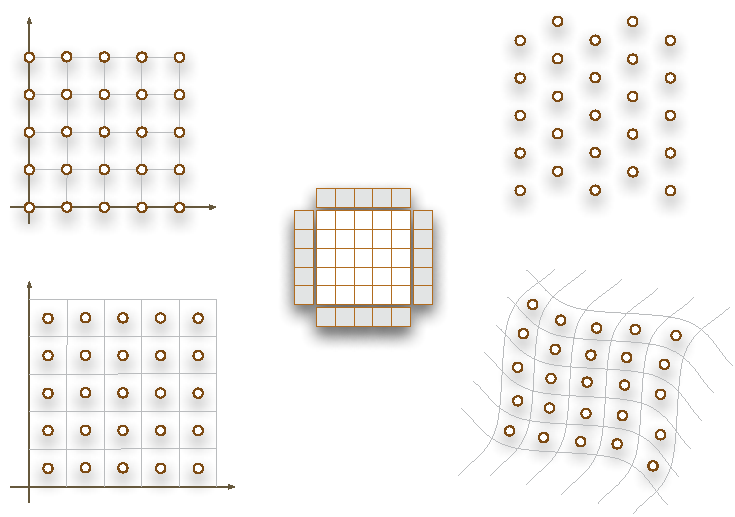
\includegraphics[scale=0.5]{figures/structured.pdf}
  \end{figure} 
%
\end{frame}

% --------------------------------------
% advantages
\begin{frame}[fragile]
%
  \frametitle{Advantages and disadvantages}
%
  \begin{itemize}
%
  \item advantages: logically rectangular
    \begin{itemize}
    \item indexing: easy traversal using loops
    \item fixed stride: predictable memory layout
    \item topology: finding neighbors is trivial
    \end{itemize}
%
    \item disadvantages: many problems don't fit in simple boxes...
      \begin{itemize}
      \item non-trivial geometries are hard to model
      \item the representational simplicity disappears quickly as modeling complexity increases
        \begin{itemize}
        \item domain feature resolution
        \item complex initial and boundary conditions 
        \item adaptive refinement: allowing the properties of the solution to direct where
          computational resources are spent
        \end{itemize}
      \end{itemize}
% 
  \end{itemize}
%
\end{frame}

% --------------------------------------
% data layout
\begin{frame}[fragile]
%
  \frametitle{Data layout and performance}
%
  \begin{itemize}
%
  \item in multi-tier memory architectures
    \begin{itemize}
    \item good data locality enables efficient cache use
    \end{itemize}
%
  \item multi-dimensional arrays: na\"ive implementations do not perform well
    \begin{itemize}
    \item for large problem sizes
    \item for complex physics updates that require keeping track of multiple fields
    \end{itemize}
%
  \item representing scalar, vector and tensor fields
    \begin{itemize}
    \item optimal layout is problem dependent
    \item goal is to minimize cache misses while updating the fields
    \end{itemize}
%
  \item the conventional mapping to arrays lays out the data in matrix form
    \begin{itemize}
    \item not necessarily the most convenient convention
    \end{itemize}
%
  \item take ownership of the indexing function
% 
  \end{itemize}
%
  \begin{figure}
    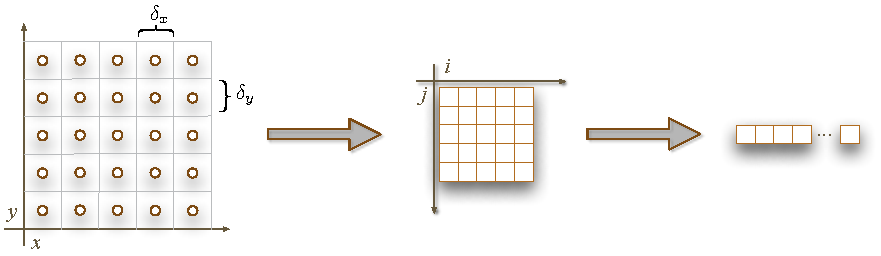
\includegraphics[scale=0.7]{figures/structured-coordinates.pdf}
  \end{figure} 
%
\end{frame}

% --------------------------------------
% updates
\begin{frame}[fragile]
%
  \frametitle{Updating the grid}
%
  \begin{itemize}
%
  \item two broad categories of problems
    \begin{itemize}
      \item steady state problems: iterates represent progress towards enforcing a spatial
        relationship dictated by the differential equation
      \item time dependent problems: iterates represent the time evolution of the solution to
        the spatial problem
    \end{itemize}
%
  \item two broad strategies:
    \begin{itemize}
      \item {\em implicit} solvers cast the constraints among iterates as a large system of
        simultaneous equations
      \item {\em explicit} solvers keep track of only a small number of the iterates
        and use them to advance the solution one step at a time
    \end{itemize}
%
  \item the complexity of the update determines the {\em stencil}
% 
  \end{itemize}
%
  \begin{figure}
    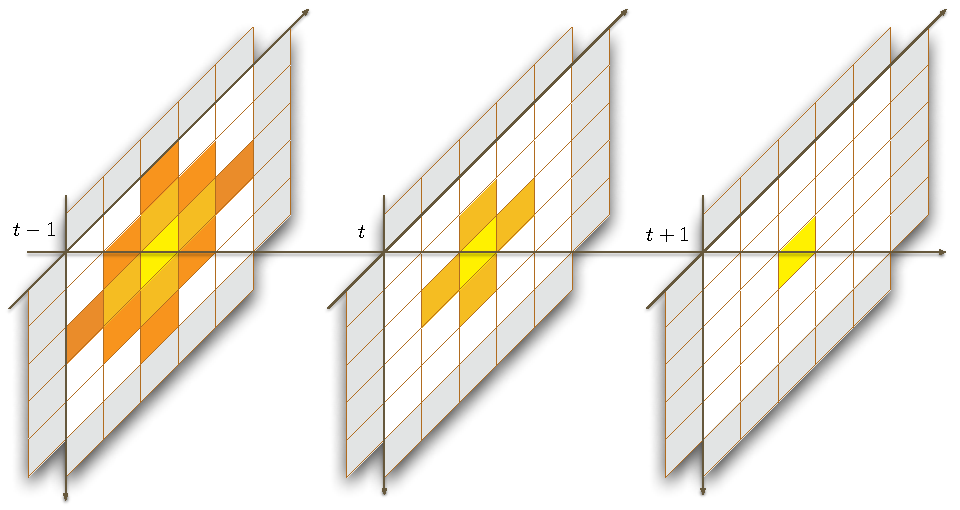
\includegraphics[scale=0.4]{figures/structured-updates.pdf}
  \end{figure} 
%
\end{frame}

% --------------------------------------
% numerics
\begin{frame}[fragile]
%
  \frametitle{Computing derivatives}
%
  \begin{itemize}
%
  \item there are three different first order approximations
    \begin{itemize}
%
    \item forward difference:
      \begin{equation}
      \partial \raisebox{-.4em}{
\includegraphics{figures/structured-1d-centered.pdf}}
      =
      \frac{1}{\delta}
      \left(
        \raisebox{-.4em}{
\includegraphics{figures/structured-1d-right.pdf}} 
        -
        \raisebox{-.4em}{
\includegraphics{figures/structured-1d-middle.pdf}} 
      \right)
      \end{equation}
%
    \item backward difference:
      \begin{equation}
      \partial \raisebox{-.4em}{
\includegraphics{figures/structured-1d-centered.pdf}}
      =
      \frac{1}{\delta}
      \left(
        \raisebox{-.4em}{
\includegraphics{figures/structured-1d-middle.pdf}} 
        -
        \raisebox{-.4em}{
\includegraphics{figures/structured-1d-left.pdf}} 
      \right)
      \end{equation}
%
    \item central difference:
      \begin{equation}
      \partial \raisebox{-.4em}{
\includegraphics{figures/structured-1d-centered.pdf}}
      =
      \frac{1}{2\delta}
      \left(
        \raisebox{-.4em}{
\includegraphics{figures/structured-1d-right.pdf}} 
        -
        \raisebox{-.4em}{
\includegraphics{figures/structured-1d-left.pdf}} 
      \right)
      \end{equation}
%
    \end{itemize}
    where $\delta$ is the uniform grid spacing
%
    \item forward and backward differences are most often used for {\em explicit} time
      integration
%
    \item central differences are used to compute spatial derivatives
%
    \item the second order central difference is given by
      \begin{equation}
      \partial \raisebox{-.2em}{
\includegraphics{figures/structured-1d-5c.pdf}}
      =
      \frac{1}{12\delta}
      \left(
        -
        \raisebox{-.2em}{\includegraphics{figures/structured-1d-55.pdf}} 
        +
        8 \raisebox{-.2em}{\includegraphics{figures/structured-1d-54.pdf}} 
        -
        8 \raisebox{-.2em}{\includegraphics{figures/structured-1d-52.pdf}} 
        +
        \raisebox{-.2em}{\includegraphics{figures/structured-1d-51.pdf}} 
      \right)
      \end{equation}
%
  \end{itemize}
%
\end{frame}

% --------------------------------------
% numerics
\begin{frame}[fragile]
%
  \frametitle{Partial derivatives in two dimensions}
%
  \begin{itemize}
%
  \item let $\delta_{x}$ and $\delta_{y}$ be the uniform grid spacing along each dimension
%
  \item then, the first order central difference approximations to the spatial derivatives are
    given by
    \begin{eqnarray}
      \partial_{x} \raisebox{-.5em}{\includegraphics{figures/structured-2d-middle.pdf}}
      & = &
      \frac{1}{2\delta_{x}}
      \left(
        \raisebox{-.5em}{\includegraphics{figures/structured-2d-e.pdf}} 
        - \raisebox{-.5em}{\includegraphics{figures/structured-2d-w.pdf}} 
      \right )
      \\
      \partial_{y} \raisebox{-.5em}{\includegraphics{figures/structured-2d-middle.pdf}}
      & = &
      \frac{1}{2\delta_{y}}
      \left(
        \raisebox{-.5em}{\includegraphics{figures/structured-2d-s.pdf}} 
        - \raisebox{-.5em}{\includegraphics{figures/structured-2d-n.pdf}} 
      \right )
    \end{eqnarray}
%
  \item and the second order derivatives are given by
    \begin{eqnarray}
      \partial_{xx} \raisebox{-.5em}{\includegraphics{figures/structured-2d-middle.pdf}}
      & = &
      \frac{1}{\delta_{x}^{2}}
      \left(
        \raisebox{-.5em}{\includegraphics{figures/structured-2d-e.pdf}} 
        -2 \raisebox{-.5em}{\includegraphics{figures/structured-2d-middle.pdf}} 
        + \raisebox{-.5em}{\includegraphics{figures/structured-2d-w.pdf}} 
      \right )
      \\
      \partial_{yy} \raisebox{-.5em}{\includegraphics{figures/structured-2d-middle.pdf}}
      & = &
      \frac{1}{\delta_{y}^{2}}
      \left(
        \raisebox{-.5em}{\includegraphics{figures/structured-2d-s.pdf}} 
        -2 \raisebox{-.5em}{\includegraphics{figures/structured-2d-middle.pdf}} 
        + \raisebox{-.5em}{\includegraphics{figures/structured-2d-n.pdf}} 
      \right )
      \\
      \partial_{xy} \raisebox{-.5em}{\includegraphics{figures/structured-2d-middle.pdf}}
      & = &
      \frac{1}{4\delta_{x}\delta_{y}}
      \left(
        \raisebox{-.5em}{\includegraphics{figures/structured-2d-se.pdf}} 
        - \raisebox{-.5em}{\includegraphics{figures/structured-2d-ne.pdf}} 
        - \raisebox{-.5em}{\includegraphics{figures/structured-2d-sw.pdf}} 
        + \raisebox{-.5em}{\includegraphics{figures/structured-2d-nw.pdf}} 
      \right )
    \end{eqnarray}
% 
  \end{itemize}
%
\end{frame}

% --------------------------------------
% example
\begin{frame}[fragile]
%
  \frametitle{Solving a simple PDE on a uniform structured grid}
%
  \begin{itemize}
%
  \item Laplace equation over some domain $\Omega \in \mathbb{R}^{d}$, subject to Dirichlet
    boundary conditions
    \begin{equation}
      \begin{array}{ccc}
      \nabla^{2} \phi = 0 & {\rm with} & \phi(\partial \Omega) = f
      \end{array}
      \label{eq:laplace}
    \end{equation}
%
  \item let the grid be uniform: $\delta_{x} =  \delta_{y}$
%
  \item in two dimensions, using first order central differences, \eqref{laplace} becomes
    \begin{eqnarray}
      (\partial_{xx} + \partial_{yy})
      \raisebox{-.5em}{\includegraphics{figures/structured-2d-middle.pdf}}
      & = &
      0
      \\
      4 \raisebox{-.5em}{\includegraphics{figures/structured-2d-middle.pdf}} 
      & = &
      \raisebox{-.5em}{\includegraphics{figures/structured-2d-e.pdf}} 
      + \raisebox{-.5em}{\includegraphics{figures/structured-2d-w.pdf}} 
      + \raisebox{-.5em}{\includegraphics{figures/structured-2d-s.pdf}} 
      + \raisebox{-.5em}{\includegraphics{figures/structured-2d-n.pdf}} 
    \end{eqnarray}
%
  \item and translates into the following constraint among grid elements
    \begin{equation}
      \raisebox{-.5em}{\includegraphics{figures/structured-2d-middle.pdf}}
      =
      \frac{1}{4}
      \raisebox{-.5em}{\includegraphics{figures/structured-2d-average.pdf}} 
      \label{eq:laplace-central}
    \end{equation}
    using a shorthand for the sum of the neighboring cells
%
  \end{itemize}
%
\end{frame}

% --------------------------------------
% example
\begin{frame}[fragile]
%
  \frametitle{An example}
%
  \begin{itemize}
%
% 
  \item specifically,
    \begin{itemize}
    \item let $\Omega$ be the unit box in two dimensions
    \item and let $\phi$ satisfy the following boundary conditions
      \begin{equation}
        \begin{array}{rcrcll}
          & & \phi(x,0) & = & \sin(\pi x)           & 0 \leq x \leq 1 \\
          & & \phi(x,1) & = & e^{-\pi} \sin(\pi x)  & 0 \leq x \leq 1 \\
          \phi(0,y) & = & \phi(1, y) & = & 0        & 0 \leq y \leq 1
        \end{array}
      \end{equation}
    \end{itemize}
%
  \item the exact solution is given by
    \begin{equation}
      \phi(x,y) = e^{-\pi y} \sin(\pi x)
    \end{equation}
%
  \item we will solve this equation using the Jacobi iterative scheme:
    \begin{itemize}
    \item make an initial guess for $\phi$ over a discretization of $\Omega$
    \item apply the boundary conditions
    \item interpret \eqref{laplace-central} as an update step to compute the next iteration
      \begin{equation}
      \raisebox{-.5em}{\includegraphics{figures/structured-2d-centered.pdf}}_{t}
      =
      \frac{1}{4}
      \raisebox{-.5em}{\includegraphics{figures/structured-2d-average.pdf}}_{t-1}
      \end{equation}
    \item stop when a convergence criterion is met
    \end{itemize}
%
  \end{itemize}
%
\end{frame}

% end of file 

%% -*- LaTeX -*-
% -*- coding: utf-8 -*-
%
% michael a.g. aïvázis
% california institute of technology
% (c) 1998-2012 all rights reserved
%

\lecture{Structured grids}{20120215}

% --------------------------------------
% example
\begin{frame}[fragile]
%
  \frametitle{Solving a simple PDE on a uniform structured grid}
%
  \begin{itemize}
%
  \item Laplace equation over some domain $\Omega \in \mathbb{R}^{d}$, subject to Dirichlet
    boundary conditions
    \begin{equation}
      \begin{array}{ccc}
      \nabla^{2} \phi = 0 & {\rm with} & \phi(\partial \Omega) = f
      \end{array}
      \label{eq:laplace}
    \end{equation}
%
  \item let the grid be uniform: $\delta_{x} =  \delta_{y}$
%
  \item in two dimensions, using first order central differences, \eqref{laplace} becomes
    \begin{eqnarray}
      (\partial_{xx} + \partial_{yy})
      \raisebox{-.5em}{\includegraphics{figures/structured-2d-middle.pdf}}
      & = &
      0
      \\
      4 \raisebox{-.5em}{\includegraphics{figures/structured-2d-middle.pdf}} 
      & = &
      \raisebox{-.5em}{\includegraphics{figures/structured-2d-e.pdf}} 
      + \raisebox{-.5em}{\includegraphics{figures/structured-2d-w.pdf}} 
      + \raisebox{-.5em}{\includegraphics{figures/structured-2d-s.pdf}} 
      + \raisebox{-.5em}{\includegraphics{figures/structured-2d-n.pdf}} 
    \end{eqnarray}
%
  \item and translates into the following constraint among grid elements
    \begin{equation}
      \raisebox{-.5em}{\includegraphics{figures/structured-2d-middle.pdf}}
      =
      \frac{1}{4}
      \raisebox{-.5em}{\includegraphics{figures/structured-2d-average.pdf}} 
      \label{eq:laplace-central}
    \end{equation}
    using a shorthand for the sum of the neighboring cells
%
  \end{itemize}
%
\end{frame}

% --------------------------------------
% example
\begin{frame}[fragile]
%
  \frametitle{An example}
%
  \begin{itemize}
%
% 
  \item specifically,
    \begin{itemize}
    \item let $\Omega$ be the unit box in two dimensions
    \item and let $\phi$ satisfy the following boundary conditions
      \begin{equation}
        \begin{array}{rcrcll}
          & & \phi(x,0) & = & \sin(\pi x)           & 0 \leq x \leq 1 \\
          & & \phi(x,1) & = & e^{-\pi} \sin(\pi x)  & 0 \leq x \leq 1 \\
          \phi(0,y) & = & \phi(1, y) & = & 0        & 0 \leq y \leq 1
        \end{array}
      \end{equation}
    \end{itemize}
%
  \item the exact solution is given by
    \begin{equation}
      \phi(x,y) = e^{-\pi y} \sin(\pi x)
    \end{equation}
%
  \item we will solve this equation using the Jacobi iterative scheme:
    \begin{itemize}
    \item make an initial guess for $\phi$ over a discretization of $\Omega$
    \item apply the boundary conditions
    \item interpret \eqref{laplace-central} as an update step to compute the next iteration
      \begin{equation}
      \raisebox{-.5em}{\includegraphics{figures/structured-2d-centered.pdf}}_{t}
      =
      \frac{1}{4}
      \raisebox{-.5em}{\includegraphics{figures/structured-2d-average.pdf}}_{t-1}
      \end{equation}
    \item stop when a convergence criterion is met
    \end{itemize}
%
  \end{itemize}
%
\end{frame}

% --------------------------------------
% the solution
\begin{frame}[fragile]
%
  \frametitle{The solution}
%
  \begin{figure}
    \centering
    \includegraphics[width=0.9\linewidth]{figures/laplace-example.pdf}
    \label{fig:reduction-shared}
  \end{figure}
%
\end{frame}


% --------------------------------------
% parallelizing
\begin{frame}[fragile]
%
  \frametitle{Implementation strategy}
%
  \begin{itemize}
%
  \item grid resolution:
    \begin{itemize}
     \item ideally determined by analyzing the boundary conditions, since discrete sampling may
       wash out sharp features
     \item for our simple example, this can be done as part of the solver initialization
     \item we will use an $N \times N$ grid and let $N$ be user specified so we can control the
       problem size
       \begin{equation}
         \delta_{x} = \delta_{y} = \frac{1}{N-1}
       \end{equation}
     \end{itemize}
%
  \item data layout
    \begin{itemize}
    \item investigate the effect of data locality by trying out various layouts
    \end{itemize}
%
  \item setting up the update
    \begin{itemize}
      \item we only need to keep track of two iterants
      \item can be done in place; do you see how?
    \end{itemize}
%
  \item convergence criterion
    \begin{itemize}
    \item we will stop iterating when
      \begin{equation}
        \maximum{\Omega} (\phi_{t} - \phi_{t-1})) < \epsilon
      \end{equation}
      and let the user specify $\epsilon$
    \end{itemize}
%
  \end{itemize}
% 
\end{frame}

%
% \begin{figure}
%   \centering
%   \includegraphics[scale=0.5]{figures/structured-dirichlet.pdf}
% \end{figure}

% --------------------------------------
% parallelization
\begin{frame}[fragile]
%
  \frametitle{Parallelization}
%
  \begin{itemize}
%
  \item the finest grain of work is clearly the cell update based on the value of its four
    nearest neighbors
%
  \item the shared memory implementation requires
    \begin{itemize}
    \item a scheme so that threads can update cells without the need for locks
    \item while maximizing locality of data access
    \item even the computation of the convergence criterion can be parallelized
    \end{itemize}
%
  \item with \mpi
    \begin{itemize}
    \item must partition the mesh among processes
    \item each process work on its own subgrid
    \item communication is required every iteration
    \item parallel convergence testing involves a collective operation
    \end{itemize}
%
  \end{itemize}
%
  \begin{figure}
    \includegraphics[scale=0.4]{figures/structured-partitioning.pdf}
  \end{figure} 
% 
\end{frame}

% --------------------------------------
% sequential
\begin{frame}[fragile]
%
  \frametitle{Sequential implementation - user interface}
%
  \begin{lstlisting}[language=c++,name=seq:frame,firstnumber=77]
// main program
int main(int argc, char* argv[]) {
    // default values for our user configurable settings
    size_t N = 10;
    double tolerance = 1.0e-6;
    const char* filename = "laplace.csv";

    // read the command line
    int command;
    while ((command = getopt(argc, argv, "N:e:o:")) != -1) {
        switch (command) {
        // get the convergence tolerance
        case 'e':
            tolerance = atof(optarg);
            break;
        // get the grid size
        case 'N':
            N = (size_t) atof(optarg);
            break;
        // get the name of the output file
        case 'o':
            filename = optarg;
        }
    }
    
  \end{lstlisting}
% 
\end{frame}

% --------------------------------------
% sequential
\begin{frame}[fragile]
%
  \frametitle{Sequential implementation - driving the solver}
%
  \begin{lstlisting}[language=c++,name=seq:frame]
    // allocate space for the solution
    Grid potential(N);

    // initialize and apply our boundary conditions
    initialize(potential);

    // call the solver
    laplace(potential, tolerance);

    // open a stream to hold the answer
    std::fstream output(filename, std::ios_base::out);

    // build a visualizer and render the solution in our chosen format
    Visualizer visualizer;
    visualizer.csv(potential, output);

    // all done
    return 0;
}
  \end{lstlisting}
% 
\end{frame}

% --------------------------------------
% sequential
\begin{frame}[fragile]
%
  \frametitle{Sequential implementation - the preamble}
%
  \begin{itemize}
  \item back up to the beginning of the file
    \begin{lstlisting}[language=c++,name=seq:frame, firstnumber=1]
#include <getopt.h>
#include <cmath>
#include <cstdlib>
#include <fstream>
#include <iostream>

// forward declarations
class Grid;
class Visualizer;

// the solver; does nothing for the time being
void initialize(Grid & grid) {};
void laplace(Grid & grid, double tolerance){};

    \end{lstlisting}
%
  \item we have separated out {\em visualization} in a different object to support different
    formats without disturbing the data representation
%
  \item \identifier{initialize} and \identifier{laplace} have trivial implementations for now
    \begin{itemize}
    \item enables testing the scaffolding without worrying about the solver
      implementation just yet
    \end{itemize}
  \end{itemize}
% 
\end{frame}

% --------------------------------------
% sequential
\begin{frame}[fragile]
%
  \frametitle{Sequential implementation - the grid object stub}
%
  \begin{lstlisting}[language=c++,name=seq:frame]
// the solution representation
class Grid {
    // interface: TBD
public:

    // meta methods
public:
    Grid(size_t size);
    ~Grid();

    // private data members: TBD
private:

    // disabled interface
    // grid will own dynamic memory, so don't let the compiler screw up
private:
    Grid(const Grid &);
    const Grid & operator= (const Grid &);
};

// the grid implementation
Grid::Grid(size_t size) {
}

Grid::~Grid() {
}

  \end{lstlisting}
% 
\end{frame}

% --------------------------------------
% sequential
\begin{frame}[fragile]
%
  \frametitle{Sequential implementation - the visualizer stub}
%
  \begin{lstlisting}[language=c++,name=seq:frame, firstnumber=97]
// the visualizer class
class Visualizer {
    // local type aliases
public:
    typedef std::ostream stream_t;

    // interface
public:
    void csv(const Grid & grid, stream_t & stream);

    // meta methods
public:
    inline Visualizer() {}
};

// the Visualizer class implementation
void Visualizer::csv(const Grid & grid, Visualizer::stream_t & stream) {
    return;
}
  \end{lstlisting}
%

\begin{itemize}
\item the code now compiles and links
  \begin{itemize}
  \item consistency check that the object collaborations are ok, for now
  \item can be tested for command line option parsing
  \end{itemize}
\end{itemize}
% 
\end{frame}

% end of file 

%% -*- LaTeX -*-
% -*- coding: utf-8 -*-
%
% michael a.g. aïvázis
% california institute of technology
% (c) 1998-2012 all rights reserved
%

\lecture{Structured grids}{20120217}

% --------------------------------------
% sequential
\begin{frame}[fragile]
%
  \frametitle{Sequential implementation - user interface}
%
  \begin{lstlisting}[language=c++,name=seq:frame,firstnumber=77]
// main program
int main(int argc, char* argv[]) {
    // default values for our user configurable settings
    size_t N = 10;
    double tolerance = 1.0e-6;
    const char* filename = "laplace.csv";

    // read the command line
    int command;
    while ((command = getopt(argc, argv, "N:e:o:")) != -1) {
        switch (command) {
        // get the convergence tolerance
        case 'e':
            tolerance = atof(optarg);
            break;
        // get the grid size
        case 'N':
            N = (size_t) atof(optarg);
            break;
        // get the name of the output file
        case 'o':
            filename = optarg;
        }
    }
    
  \end{lstlisting}
% 
\end{frame}

% --------------------------------------
% sequential
\begin{frame}[fragile]
%
  \frametitle{Sequential implementation - driving the solver}
%
  \begin{lstlisting}[language=c++,name=seq:frame]
    // allocate space for the solution
    Grid potential(N);

    // initialize and apply our boundary conditions
    initialize(potential);

    // call the solver
    laplace(potential, tolerance);

    // open a stream to hold the answer
    std::fstream output(filename, std::ios_base::out);

    // build a visualizer and render the solution in our chosen format
    Visualizer visualizer;
    visualizer.csv(potential, output);

    // all done
    return 0;
}
  \end{lstlisting}
% 
\end{frame}

% --------------------------------------
% sequential
\begin{frame}[fragile]
%
  \frametitle{Sequential implementation - the preamble}
%
  \begin{itemize}
  \item back up to the beginning of the file
    \begin{lstlisting}[language=c++,name=seq:frame, firstnumber=1]
#include <getopt.h>
#include <cmath>
#include <cstdlib>
#include <fstream>
#include <iostream>

// forward declarations
class Grid;
class Visualizer;

// the solver; does nothing for the time being
void initialize(Grid & grid) {};
void laplace(Grid & grid, double tolerance){};

    \end{lstlisting}
%
  \item we have separated out {\em visualization} in a different object to support different
    formats without disturbing the data representation
%
  \item \identifier{initialize} and \identifier{laplace} have trivial implementations for now
    \begin{itemize}
    \item enables testing the scaffolding without worrying about the solver
      implementation just yet
    \end{itemize}
  \end{itemize}
% 
\end{frame}

% --------------------------------------
% sequential
\begin{frame}[fragile]
%
  \frametitle{Sequential implementation - the grid object stub}
%
  \begin{lstlisting}[language=c++,name=seq:frame]
// the solution representation
class Grid {
    // interface: TBD
public:

    // meta methods
public:
    Grid(size_t size);
    ~Grid();

    // private data members: TBD
private:

    // disabled interface
    // grid will own dynamic memory, so don't let the compiler screw up
private:
    Grid(const Grid &);
    const Grid & operator= (const Grid &);
};

// the grid implementation
Grid::Grid(size_t size) {
}

Grid::~Grid() {
}

  \end{lstlisting}
% 
\end{frame}

% --------------------------------------
% sequential
\begin{frame}[fragile]
%
  \frametitle{Sequential implementation - the visualizer stub}
%
  \begin{lstlisting}[language=c++,name=seq:frame, firstnumber=97]
// the visualizer class
class Visualizer {
    // local type aliases
public:
    typedef std::ostream stream_t;

    // interface
public:
    void csv(const Grid & grid, stream_t & stream);

    // meta methods
public:
    inline Visualizer() {}
};

// the Visualizer class implementation
void Visualizer::csv(const Grid & grid, Visualizer::stream_t & stream) {
    return;
}
  \end{lstlisting}
%

\begin{itemize}
\item the code now compiles and links
  \begin{itemize}
  \item consistency check that the object collaborations are ok, for now
  \item can be tested for command line option parsing
  \end{itemize}
\end{itemize}
% 
\end{frame}

% --------------------------------------
% the grid initializer
\begin{frame}[fragile]
%
  \frametitle{Fleshing out the initializer}
%
  \begin{lstlisting}[language=c++,name=seq:initializer]
// the grid initializer:
// clear the grid contents and apply our boundary conditions 
void initialize(Grid & grid) {
    // ask the grid to clear its memory
    grid.clear(1.0);
    // apply the dirichlet conditions
    for (size_t cell=0; cell < grid.size(); cell++) {
        // evaluate sin(pi x)
        double sin = std::sin(cell * grid.delta() * pi);
        // along the x axis, at top and  bottom
        grid(cell, 0) = sin;
        grid(cell, grid.size()-1) = sin * std::exp(-pi);
        // along the y axis, left and right
        grid(0, cell) = 0.0;
        grid(grid.size()-1, cell) = 0.0;
    }

    return;
}
  \end{lstlisting}
%
  \begin{itemize}
  \item the grid knows its size, its spacing $\delta$, and can initialize its memory
  \item access to grid elements happens through an overloaded \identifier{operator()} so we can
    {\em encapsulate} the indexing function
  \end{itemize}
%
\end{frame}

% --------------------------------------
% the grid declaration
\begin{frame}[fragile]
%
  \frametitle{The grid class declaration}
%
  \begin{lstlisting}[language=c++,name=seq:grid,firstnumber=29]
// the solution representation
class Grid {
    // interface
public:
    // set all cells to the specified value
    void clear(double value=0.0);
    // the grid dimensions
    size_t size() const {return _size;}
    // the grid spacing
    double delta() const {return _delta;}
    // access to the cells
    double & operator()(size_t i, size_t j) {return _block[j*_size+i];}
    double operator()(size_t i, size_t j) const {return _block[j*_size+i];}
    // meta methods
public:
    Grid(size_t size);
    ~Grid();
    // data members
private:
    const size_t _size;
    const double _delta;
    double* _block;
    // disable these
private:
    Grid(const Grid &);
    const Grid & operator= (const Grid &);
};

  \end{lstlisting}
%
\end{frame}

% --------------------------------------
% the grid implementation
\begin{frame}[fragile]
%
  \frametitle{The grid class implementation}
%
  \begin{lstlisting}[language=c++,name=seq:grid]
// the grid implementation
// interface
void Grid::clear(double value) {
    for (size_t i=0; i < _size*_size; i++) {
        _block[i] = value;
    }

    return;
}

// constructor
Grid::Grid(size_t size) :
    _size(size), 
    _delta((1.0 - 0.0)/(size-1)),
    _block(new double[size*size]) {
}

// destructor
Grid::~Grid() {
    delete [] _block;
}

  \end{lstlisting}
%
\end{frame}

% --------------------------------------
% the grid visualizer
\begin{frame}[fragile]
%
  \frametitle{Grid visualization}
%
  \begin{lstlisting}[language=c++,name=seq:visualizer,firstnumer=97]
// the visualizer class
class Visualizer {
    // local type aliases
public:
    typedef std::ostream stream_t;
    // interface
public:
    void csv(const Grid & grid, stream_t & stream);
    // meta methods
public:
    inline Visualizer() {}
};

// the Visualizer class implementation
void Visualizer::csv(const Grid & grid, Visualizer::stream_t & stream) {
    for (size_t j=0; j < grid.size(); j++) {
        stream << j;
        for (size_t i=0; i < grid.size(); i++) {
            stream << "," << grid(i,j);
        }
        stream << std::endl;
    }

    return;
}

  \end{lstlisting}
%
\end{frame}

% --------------------------------------
% the results of initialization
\begin{frame}[fragile]
%
  \frametitle{Printing out the initial grid}
%
  \begin{itemize}
  \item we should be able to print out the initialized grid
%
  \begin{shell}{}
#> mm laplace
#> laplace
#> cat laplace.csv
0,0,0.3827,0.7071,0.9239,1,0.9239,0.7071,0.3827,1.225e-16
1,0,1,1,1,1,1,1,1,0
2,0,1,1,1,1,1,1,1,0
3,0,1,1,1,1,1,1,1,0
4,0,1,1,1,1,1,1,1,0
5,0,1,1,1,1,1,1,1,0
6,0,1,1,1,1,1,1,1,0
7,0,1,1,1,1,1,1,1,0
8,0,0.01654,0.0306,0.03992,0.04321,0.0399,0.03056,0.01654,0
  \end{shell}
%
  \item notice that
    \begin{itemize}
    \item the top line contains some recognizable values
    \item the left and right borders are set to zero
    \item the interior of the grid is painted with our initial guess
    \end{itemize}
%
  \item still to do:
    \begin{itemize}
    \item write the update
    \item build a grid with the exact solution 
    \item build the error field (why?)
    \end{itemize}
  \end{itemize}
%
\end{frame}

% end of file 

%% -*- LaTeX -*-
% -*- coding: utf-8 -*-
%
% michael a.g. aïvázis
% california institute of technology
% (c) 1998-2012 all rights reserved
%

\lecture{Sequential implementation of the Jacobi solver}{20120222}

% --------------------------------------
% the grid declaration
\begin{frame}[fragile]
%
  \frametitle{The grid class declaration}
%
  \begin{lstlisting}[language=c++,name=seq:grid,firstnumber=29]
// the solution representation
class Grid {
    // interface
public:
    // set all cells to the specified value
    void clear(double value=0.0);
    // the grid dimensions
    size_t size() const {return _size;}
    // the grid spacing
    double delta() const {return _delta;}
    // access to the cells
    double & operator()(size_t i, size_t j) {return _block[j*_size+i];}
    double operator()(size_t i, size_t j) const {return _block[j*_size+i];}
    // meta methods
public:
    Grid(size_t size);
    ~Grid();
    // data members
private:
    const size_t _size;
    const double _delta;
    double* _block;
    // disable these
private:
    Grid(const Grid &);
    const Grid & operator= (const Grid &);
};

  \end{lstlisting}
%
\end{frame}

% --------------------------------------
% the grid implementation
\begin{frame}[fragile]
%
  \frametitle{The grid class implementation}
%
  \begin{lstlisting}[language=c++,name=seq:grid]
// the grid implementation
// interface
void Grid::clear(double value) {
    for (size_t i=0; i < _size*_size; i++) {
        _block[i] = value;
    }

    return;
}

// constructor
Grid::Grid(size_t size) :
    _size(size), 
    _delta((1.0 - 0.0)/(size-1)),
    _block(new double[size*size]) {
}

// destructor
Grid::~Grid() {
    delete [] _block;
}

  \end{lstlisting}
%
\end{frame}

% --------------------------------------
% the solver
\begin{frame}[fragile]
%
  \frametitle{Fleshing out the solver}
%
  \begin{lstlisting}[language=c++,basicstyle=\tt\bfseries\tiny,name=seq:solver,firstnumber=169]
// the solver driver
void laplace(Grid & current, double tolerance) {
    // create and initialize temporary storage
    Grid next(current.size());
    initialize(next);
    // put an upper bound on the number of iterations
    long max_iterations = (long) 1e4;;
    for (long iterations = 0; iterations<max_iterations; iterations++) {
        double max_dev = 0.0;
        // do an iteration step
        // leave the boundary alone
        // iterate over the interior of the grid
        for (size_t j=1; j < current.size()-1; j++) {
            for (size_t i=1; i < current.size()-1; i++) {
                // update
                next(i,j) = 0.25*(
                    current(i+1,j)+current(i-1,j)+current(i,j+1)+current(i,j-1));
                // compute the deviation from the last generation
                double dev = std::abs(next(i,j) - current(i,j));
                // and update the maximum deviation
                if (dev > max_dev) {
                    max_dev = dev;
                }
            }
        }
        // swap the blocks between the two grids
        Grid::swapBlocks(current, next);
        // check covergence
        if (max_dev < tolerance) {
            break;
        }
    }
    return;
}
  \end{lstlisting}
%
\end{frame}

% --------------------------------------
% the updated grid class
\begin{frame}[fragile]
%
  \frametitle{Adding the new grid interface}
%
  \begin{itemize}
  \item here is the declaration of \function{Grid::swapBlocks}
%
    \begin{lstlisting}[language=c++,firstnumber=30]
class Grid {
    // interface
    public:
    ...
    // exchange the data blocks of two compatible grids
    static void swapBlocks(Grid &, Grid &);
    ...
};
    \end{lstlisting}
%
  \item and its definition
%
    \begin{lstlisting}[language=c++,firstnumber=69]
void Grid::swapBlocks(Grid & g1, Grid & g2) {
    // bail out if the two operands are not compatible
    if (g1.size() != g2.size()) {
        throw "Grid::swapblocks: size mismatch";
    }
    if (g1.delta() != g2.delta()) {
        throw "Grid::swapblocks: spacing mismatch";
    }
    // but if they are, just exhange their data buffers
    double * temp = g1._block;
    g1._block = g2._block;
    g2._block = temp;
    // all done
    return;
}
    \end{lstlisting}
%
  \end{itemize}
%
\end{frame}

% --------------------------------------
% rework the driver to print out the exact solution and the error field
\begin{frame}[fragile]
%
  \frametitle{Reworking the driver}
%
  \begin{lstlisting}[language=c++,basicstyle=\tt\bfseries\tiny,name=seq:driver,firstnumber=239]
    // build a visualizer
    Visualizer vis;

    // compute the exact solution
    Grid solution(N);
    exact(solution);
    std::fstream exact_stream("exact.csv", std::ios_base::out);
    vis.csv(solution, exact_stream);
    
    // allocate space for the solution
    Grid potential(N);
    // initialize and apply our boundary conditions
    initialize(potential);
    // call the solver
    laplace(potential, tolerance);
    // open a stream to hold the answer
    std::fstream output_stream(filename, std::ios_base::out);
    // build a visualizer and render the solution in our chosen format
    vis.csv(potential, output_stream);

    // compute the error field
    Grid error(N);
    relative_error(potential, solution, error);
    std::fstream error_stream("error.csv", std::ios_base::out);
    vis.csv(error, error_stream);

    // all done
    return 0;
}
  \end{lstlisting}
%
\end{frame}

% --------------------------------------
% computing the exact and error fields
\begin{frame}[fragile]
% 
  \frametitle{Computing the exact solution and the error field}
%
  \begin{lstlisting}[language=c++,firstnumber=143]
void exact(Grid & grid) {
    //  paint the exact solution
    for (size_t j=0; j < grid.size(); j++) {
        for (size_t i=0; i < grid.size(); i++) {
            double x = i*grid.delta();
            double y = j*grid.delta();
            grid(i,j) = std::exp(-pi*y)*std::sin(pi*x);
        }
    }
    return;
}

void relative_error(
    const Grid & computed, const Grid & exact, Grid & error) {
    //  compute the relative error
    for (size_t j=0; j < exact.size(); j++) {
        for (size_t i=0; i < exact.size(); i++) {
            if (exact(i,j) == 0.0) { // hm... sloppy!
                error(i,j) = std::abs(computed(i,j));
            } else {
                error(i,j) = std::abs(computed(i,j) - exact(i,j))/exact(i,j);
            }
        }
    }
    return;
}

  \end{lstlisting}
%
\end{frame}

% --------------------------------------
% assessment
\begin{frame}[fragile]
%
  \frametitle{Shortcomings}
%
  \begin{itemize}
%
  \item numerics:
    \begin{itemize}
    \item it converges very slowly; other update {\em schemes} improve on this
    \item our approximation is very low order, so it takes very large grids to produce a few
      digits of accuracy
    \item the convergence criterion has some unwanted properties; it triggers
      \begin{itemize}
      \item prematurely: large swaths of constant values may never get updated
      \item it would trigger even if we were updating the wrong grid!
      \end{itemize}
    \end{itemize}
%
  \item design:
    \begin{itemize}
    \item separate the problem specification from its solution
    \item there are other objects lurking, waiting to be uncovered
    \item someone should make the graphic visualizer
    \item restarts anybody?
    \item how would you try out different convergence criteria? update schemes? memory layouts?
    \end{itemize}
%
    \item usability:
      \begin{itemize}
      \item supporting interchangeable parts requires damage to the top level driver
        \begin{itemize}
        \item to enable the user to make the selection
        \item to expose new command line arguments that configure the new parts
        \end{itemize}
      \end{itemize}
%
  \end{itemize}
%
\end{frame}

% --------------------------------------
% assessment
\begin{frame}[fragile]
%
  \frametitle{Assessing our fundamentals}
%
  \begin{itemize}
%
  \item \class{Grid} is a good starting point for abstracting structured grids
    \begin{itemize}
    \item assumes ownership of the memory associated with a structured grid
    \item encapsulates the indexing function
    \item extend it to
      \begin{itemize}
      \item support different memory layout strategies
      \item support non-square grids (?)
      \item support non-uniform grids (?)
      \item higher dimensions
      \item if you need any of these, consider using one of the many excellent class libraries
        written by experts
      \end{itemize}
    \end{itemize}
%
  \item \class{Visualizer}, under another name, can form the basis for a more general
    persistence library
    \begin{itemize}
    \item to support HDF5, NetCDF, bitmaps, voxels, etc.
    \end{itemize}
%
  \end{itemize}
%
\end{frame}

% end of file 

%% -*- LaTeX -*-
% -*- coding: utf-8 -*-
%
% michael a.g. aïvázis
% california institute of technology
% (c) 1998-2012 all rights reserved
%

\lecture{Wrapping up the sequential implementation}{20120224}

% --------------------------------------
% assessment
\begin{frame}[fragile]
%
  \frametitle{Shortcomings}
%
  \begin{itemize}
%
  \item numerics:
    \begin{itemize}
    \item it converges very slowly; other update {\em schemes} improve on this
    \item our approximation is very low order, so it takes very large grids to produce a few
      digits of accuracy
    \item the convergence criterion has some unwanted properties; it triggers
      \begin{itemize}
      \item prematurely: large swaths of constant values may never get updated
      \item it would trigger even if we were updating the wrong grid!
      \end{itemize}
    \end{itemize}
%
  \item design:
    \begin{itemize}
    \item separate the problem specification from its solution
    \item there are other objects lurking, waiting to be uncovered
    \item someone should make the graphic visualizer
    \item restarts anybody?
    \item how would you try out different convergence criteria? update schemes? memory layouts?
    \end{itemize}
%
    \item usability:
      \begin{itemize}
      \item supporting interchangeable parts requires damage to the top level driver
        \begin{itemize}
        \item to enable the user to make the selection
        \item to expose new command line arguments that configure the new parts
        \end{itemize}
      \end{itemize}
%
  \end{itemize}
%
\end{frame}

% --------------------------------------
% assessment
\begin{frame}[fragile]
%
  \frametitle{Assessing our fundamentals}
%
  \begin{itemize}
%
  \item \class{Grid} is a good starting point for abstracting structured grids
    \begin{itemize}
    \item assumes ownership of the memory associated with a structured grid
    \item encapsulates the indexing function
    \item extend it to
      \begin{itemize}
      \item support different memory layout strategies
      \item support non-square grids (?)
      \item support non-uniform grids (?)
      \item higher dimensions
      \item if you need any of these, consider using one of the many excellent class libraries
        written by experts
      \end{itemize}
    \end{itemize}
%
  \item \class{Visualizer}, under another name, can form the basis for a more general
    persistence library
    \begin{itemize}
    \item to support HDF5, NetCDF, bitmaps, voxels, etc.
    \end{itemize}
%
  \end{itemize}
%
\end{frame}

% --------------------------------------
% the Problem class
\begin{frame}[fragile]
% 
  \frametitle{The \class{Problem} class: the interface}
%
  \begin{lstlisting}[language=c++,name=Problem]
// the solution representation
class acm114::laplace::Problem {
    //typedefs
public:
    typedef std::string string_t;
    // interface
public:
    inline string_t name() const;
    inline const Grid & exact() const;
    inline const Grid & deviation() const;
    inline Grid & solution();
    inline const Grid & solution() const;
    inline Grid & error();
    inline const Grid & error() const;
    // abstract
    virtual void initialize() = 0;
    virtual void initialize(Grid &) const = 0;
    // meta methods
public:
    inline Problem(string_t name, double width, size_t points);
    virtual ~Problem();
    // data members
  \end{lstlisting}
%
\end{frame}

% --------------------------------------
% the Problem class
\begin{frame}[fragile]
% 
  \frametitle{The \class{Problem} class: the data}
%
  \begin{lstlisting}[language=c++,name=Problem]
protected:
    string_t _name;
    double _delta;
    Grid _solution;
    Grid _exact;
    Grid _error;
    Grid _deviation;
    // disable these
private:
    Problem(const Problem &);
    const Problem & operator= (const Problem &);
};
  \end{lstlisting}
%
\end{frame}

% --------------------------------------
% our specific example
\begin{frame}[fragile]
% 
  \frametitle{The \class{Example} class}
%
  \begin{lstlisting}[language=c++]
class acm114::laplace::Example : public acm114::laplace::Problem {
    // interface
public:
    virtual void initialize();
    virtual void initialize(Grid &) const;

    // meta methods
public:
    inline Example(string_t name, double width, size_t points);
    virtual ~Example();

    // disable these
private:
    Example(const Example &);
    const Example & operator= (const Example &);
};

  \end{lstlisting}
%
\end{frame}

% --------------------------------------
% the solver basis
\begin{frame}[fragile]
% 
  \frametitle{The \class{Solver} class}
%
  \begin{lstlisting}[language=c++]
class acm114::laplace::Solver {
    // interface
public:
    virtual void solve(Problem &) = 0;

    // meta methods
public:
    inline Solver();
    virtual ~Solver();

    // data members
private:

    // disable these
private:
    Solver(const Solver &);
    const Solver & operator= (const Solver &);
};

  \end{lstlisting}
%
\end{frame}

% --------------------------------------
% the jacobi solver 
\begin{frame}[fragile]
% 
  \frametitle{The \class{Jacobi} class}
%
  \begin{lstlisting}[language=c++]
class acm114::laplace::Jacobi : public acm114::laplace::Solver {
    // interface
public:
    virtual void solve(Problem &);

    // meta methods
public:
    inline Jacobi(double tolerance, size_t workers);
    virtual ~Jacobi();

    // implementation details
protected:
    virtual void _solve(Problem &);
    static void * _update(void *);

    // data members
private:
    double _tolerance;
    size_t _workers;

    // disable these
private:
    Jacobi(const Jacobi &);
    const Jacobi & operator= (const Jacobi &);
};

  \end{lstlisting}
%
\end{frame}

% --------------------------------------
% parallelization using threads
\begin{frame}[fragile]
%
  \frametitle{Parallelization using threads}
%
  \begin{itemize}
%
  \item the shared memory implementation requires
    \begin{itemize}
    \item a scheme so that threads can update cells without the need for locks
    \item while maximizing locality of data access
    \item even the computation of the convergence criterion can be parallelized
    \end{itemize}
%
  \item parallelization strategy
    \begin{itemize}
    \item we will focus on parallelizing the iterative grid update
      \begin{itemize}
      \item grid initialization, visualization, computing the exact answer and the error field
        do not depend on the {\em number of iterations}
      \end{itemize}
    \item the finest grain of work is clearly an individual cell update based on the value of
      its four nearest neighbors
    \item for this two dimensional example, we can build coarser grain tasks using
      \begin{itemize}
      \item horizontal or vertical strips
      \item non-overlapping blocks
      \item the strategy gets more complicated if you want to perform the update in place
      \end{itemize}
    \item the communication patterns are trivial for the double buffering layout; only the
      final update of the convergence criterion requires any locking
    \item each coarse grain task can be assigned to a thread
    \end{itemize}
%
  \end{itemize}
% 
\end{frame}

% --------------------------------------
% required changes to the sequential driver
\begin{frame}[fragile]
%
  \frametitle{Required changes to the sequential solution}
%
  \begin{itemize}
%
  \item what is needed
    \begin{itemize}
    \item an object to hold the problem information shared among the threads
    \item the per-thread administrative data structure that holds the thread id and the pointer
      to the shared information
      \begin{itemize}
      \item this is the argument to \function{pthread\_create}
      \end{itemize}
    \item a mutex to protect the update of the global convergence criterion
    \item a \function{pthread\_create} compatible worker routine
    \item a change at the top-level driver to enable the user to choose the number of threads
    \end{itemize}
%
  \item and a strategy for managing the thread life cycle
    \begin{itemize}
%
    \item synchronization is trivial if
      \begin{itemize}
      \item we spawn our threads to perform the updates of a single iteration
      \item harvest them
      \item check the convergence criterion 
      \item stop, or respawn them if another iteration is necessary
      \end{itemize}
%
    \item can the convergence test be done in parallel?
      \begin{itemize}
        \item so we don't have to pay the create/harvest overhead?
        \item if so, how do we guarantee correctness and consistency?
      \end{itemize}
%
    \end{itemize}
% 
  \end{itemize}
%
\end{frame}

% --------------------------------------
% the jacobi solver 
\begin{frame}[fragile]
% 
  \frametitle{Threaded \class{Jacobi}: thread data}
%
  \begin{lstlisting}[language=c++,name=Jacobi:threaded]
struct Task {
    // shared information 
    size_t workers;
    Grid & current;
    Grid & next;
    double maxDeviation;
    // mutex to control access to the convergence criterion
    pthread_mutex_t lock; 

    // constructor
    Task(size_t workers, Grid & current, Grid & next) :
        workers(workers), current(current), next(next), maxDeviation(0.0) {
        pthread_mutex_init(&lock, 0);
    }
    // destructor
    ~Task() {
        pthread_mutex_destroy(&lock);
    }
};

struct Context {
    // thread info
    size_t id;
    pthread_t descriptor;
    Task * task;
};

  \end{lstlisting}
%
\end{frame}

% --------------------------------------
% the jacobi solver 
\begin{frame}[fragile]
% 
  \frametitle{Threaded \class{Jacobi}: driving the update}
%
  \begin{lstlisting}[language=c++,name=Jacobi:threaded]
void Jacobi::solve(Problem & problem) {
    // initialize the problem
    problem.initialize();
    // do the actual solve
    _solve(problem);
    // compute and store the error
    std::cout << "  computing absolute error" << std::endl;
    //  compute the relative error
    Grid & error = problem.error();
    const Grid & exact = problem.exact();
    const Grid & solution = problem.solution();

    for (size_t j=0; j < exact.size(); j++) {
        for (size_t i=0; i < exact.size(); i++) {
            if (exact(i,j) == 0.0) {
                error(i,j) = std::abs(solution(i,j));
            } else {
                error(i,j) = std::abs(solution(i,j) - exact(i,j))/exact(i,j);
            }
        }
    }
    std::cout << " --- done." << std::endl;
    return;
}
  \end{lstlisting}
%
\end{frame}

% --------------------------------------
% the jacobi solver 
\begin{frame}[fragile]
% 
  \frametitle{Threaded \class{Jacobi}: the master thread}
%
  \begin{lstlisting}[language=c++,name=Jacobi:threaded]
void Jacobi::_solve(Problem & problem) {
    Grid & current = problem.solution();

    // create and initialize temporary storage
    Grid next(current.size());
    problem.initialize(next);

    // shared thread info
    Task task(_workers, current, next);
    // per-thread information
    Context context[_workers];

    // let's get going
    std::cout << "jacobi: tolerance=" << _tolerance << std::endl;

    // put an upper bound on the number of iterations
    const size_t max_iterations = (size_t) 1.0e4;
  \end{lstlisting}
%
\end{frame}

% --------------------------------------
% the jacobi solver 
\begin{frame}[fragile]
% 
  \frametitle{Threaded \class{Jacobi}: the master thread, part 2}
%
  \begin{lstlisting}[language=c++,name=Jacobi:threaded,basicstyle=\tt\bfseries\tiny]
    for (size_t iterations = 0; iterations<max_iterations; iterations++) {
        if (iterations % 100 == 0) {
            std::cout << "     " << iterations << std::endl;
        }
        // reset the maximium deviation
        task.maxDeviation = 0.0;
        // spawn the threads
        for (size_t tid=0; tid < _workers; tid++) {
            context[tid].id = tid;
            context[tid].task = &task;

            int status = pthread_create(&context[tid].descriptor, 0, _update, &context[tid]);
            if (status) {
                throw ("error in pthread_create");
            }
        }
        // harvest the threads
        for (size_t tid = 0; tid < _workers; tid++) {
            pthread_join(context[tid].descriptor, 0);
        }

        // swap the blocks between the two grids
        Grid::swapBlocks(current, next);
        // check covergence
        if (task.maxDeviation < _tolerance) {
            std::cout << " ### convergence in " << iterations << " iterations!" << std::endl;
            break;
        }
    }
    std::cout << " --- done." << std::endl;

    return;
}
  \end{lstlisting}
%
\end{frame}

% --------------------------------------
% the jacobi solver 
\begin{frame}[fragile]
% 
  \frametitle{Threaded \class{Jacobi}: update in the worker threads}
%
  \begin{lstlisting}[language=c++,basicstyle=\tt\bfseries\tiny,name=Jacobi:threaded]
void * Jacobi::_update(void * arg) {
    Context * context = static_cast<Context *>(arg);

    size_t id = context->id;
    Task * task = context->task;

    size_t workers = task->workers;
    Grid & current = task->current;
    Grid & next = task->next;
    pthread_mutex_t lock = task->lock;

    double max_dev = 0.0;
    // do an iteration step
    // leave the boundary alone
    // iterate over the interior of the grid
    for (size_t j=id+1; j < current.size()-1; j+=workers) {
        for (size_t i=1; i < current.size()-1; i++) {
            next(i,j) = 0.25*(current(i+1,j)+current(i-1,j)+current(i,j+1)+current(i,j-1));
            // compute the deviation from the last generation
            double dev = std::abs(next(i,j) - current(i,j));
            // and update the maximum deviation
            if (dev > max_dev) {
                max_dev = dev;
            }
        }
    }

    // grab the lock and update the global maximum deviation
    pthread_mutex_lock(&lock);
    if (task->maxDeviation < max_dev) {
        task->maxDeviation = max_dev;
    }
    pthread_mutex_unlock(&lock);

    return 0;
}
  \end{lstlisting}
%
\end{frame}

% --------------------------------------
% improving the threaded implementation
\begin{frame}[fragile]
%
  \frametitle{Assessing the threaded implementation}
%
  \begin{itemize}
%
  \item the implemented synchronization scheme is very simple
    \begin{itemize}
    \item each grid update step spawns some number of workers to update a subset of the cells
    \item the workers are harvested after the grid is updated
    \item the main thread checks for convergence
    \item if another iteration is required, a new set of workers is spawned
    \end{itemize}
%
  \item the simplicity of this strategy comes at a cost
    \begin{itemize}
    \item {\em scalability} suffers when the overhead of creating and harvesting threads is
      comparable to amount of work done by each thread
    \item for low thread counts, it is still an overall win, since the time to solution
      decreases and the machine utilization is better
    \item but as the number of threads increases, the program becomes {\em slower}
      \begin{itemize}
      \item timing a $100\times100$ grid to convergence on a recent MacPro
%
        \begin{equation*}
          \begin{array}{r|ccccc}
% header
            {\rm threads } & 1 & 2 & 4 & 8 & 16 \\
            \hline 
            {\rm time} (s) & 4.367 & 2.517 & 1.918 & 1.937 & 3.537
% 
          \end{array}
        \end{equation*}
      \item and 10,000 iterations of a $1000\times1000$ grid
        \begin{equation*}
          \begin{array}{r|ccccc}
% header
            {\rm threads } & 1 & 2 & 4 & 8 & 16 \\
            \hline 
            {\rm time} (s) & 413.306 & 211.050 & 109.509 & 98.279 & 74.087
% 
          \end{array}
        \end{equation*}
      \end{itemize}

    \end{itemize}
%
\end{itemize}
%
\end{frame}

% --------------------------------------
% Improving the update loop
\begin{frame}[fragile]
%
  \frametitle{Improving the update loop}
%
  \begin{itemize}
%
  \item the plan is to keep the workers alive and updating the grid while either we converge or
    \identifier{max\_iterations} is reached
  \item the main thread
    \begin{itemize}
    \item loops to spawn all the threads
    \item and immediately enters a loop to harvest them
    \end{itemize}
%
  \item the workers use a condition variable to synchronize among themselves
    \begin{itemize}
    \item they iterate, updating the grid
    \item grab a mutex, deposit their local maximum deviation from the last iterations, update
      a counter that records how many workers have completed their update, and release the lock
    \item enter another critical section with the termination logic
      \begin{itemize}
      \item everybody uses a condition variable to wait for the slowest worker
      \item the slowest worker checks the convergence criterion and updates the termination
        flag, swaps the grid blocks and signals everybody else
      \item if the termination flag is set, or if the maximum number of iterations has been
        reached, all threads exit
      \end{itemize}
    \end{itemize}
%
  \end{itemize}
%
\end{frame}

% --------------------------------------
% the jacobi solver 
\begin{frame}[fragile]
% 
  \frametitle{Threaded \class{Jacobi}: the main thread}
%
  \begin{lstlisting}[language=c++,name=Jacobi:updated-solve,basicstyle=\tt\bfseries\tiny]
void Jacobi::_solve(Problem & problem) {
    Grid & current = problem.solution();

    // create and initialize temporary storage
    Grid next(current.size());
    problem.initialize(next);

    // shared thread info
    Task task(_workers, _tolerance, current, next);
    // per-thread information
    Context context[_workers];
    // spawn the threads
    std::cout << "jacobi: spawning " << _workers << " workers" << std::endl;
    for (size_t tid=0; tid < _workers; tid++) {
        context[tid].id = tid;
        context[tid].task = &task;
        
        int status = pthread_create(&context[tid].descriptor, 0, _update, &context[tid]);
        if (status) {
            throw ("error in pthread_create");
        }
    }
    // harvest the threads
    for (size_t tid = 0; tid < _workers; tid++) {
            pthread_join(context[tid].descriptor, 0);
        }
    // done
    std::cout << "jacobi: done." << std::endl;
    return;
}
  \end{lstlisting}
%
\end{frame}

% --------------------------------------
% the jacobi solver 
\begin{frame}[fragile]
% 
  \frametitle{Threaded \class{Jacobi}: updated thread data}
%
  \begin{lstlisting}[language=c++,name=Jacobi:updated-threaded,basicstyle=\tt\bfseries\tiny]
struct Task {
    // shared information 
    size_t workers; // the number of threads
    double tolerance; // the covergence tolerance
    Grid & current;
    Grid & next;

    bool done; // is there more work?
    double maxDeviation; // the value
    size_t contributions; // the number of threads that have deposited contributions
    pthread_mutex_t gridUpdate_lock; //the mutex
    pthread_cond_t gridUpdate_check;

    Task(size_t workers, double tolerance, Grid & current, Grid & next) :
        workers(workers), tolerance(tolerance), current(current), next(next),
        done(false), maxDeviation(0.0), contributions(0),
        gridUpdate_lock(), gridUpdate_check() {
        // initialize the grid update lock
        pthread_mutex_init(&gridUpdate_lock, 0);
        pthread_cond_init(&gridUpdate_check, 0);
    }

    ~Task() {
        pthread_mutex_destroy(&gridUpdate_lock);
        pthread_cond_destroy(&gridUpdate_check);
    }
};

  \end{lstlisting}
%
\end{frame}

% --------------------------------------
% the jacobi solver 
\begin{frame}[fragile]
% 
  \frametitle{Threaded \class{Jacobi}: workers, part 1}
%
  \begin{lstlisting}[language=c++,name=Jacobi:updated-solve,basicstyle=\tt\bfseries\tiny]
// the threaded update
void * Jacobi::_update(void * arg) {
    Context * context = static_cast<Context *>(arg);

    size_t id = context->id;
    Task * task = context->task;

    const size_t workers = task->workers;
    Grid & current = task->current;
    Grid & next = task->next;

    size_t maxIterations = (size_t) 1e4;
    // iterate, updating the grid until done
    for (size_t iteration = 0; iteration < maxIterations; iteration++) {
        // thread 0: print an update
        if (id == 0 && iteration % 100 == 0) {
            std::cout << "    " << iteration << std::endl;
        }

        double max_dev = 0.0;
        // do an iteration step
        // leave the boundary alone
        // iterate over the interior of the grid
        for (size_t j=id+1; j < current.size()-1; j+=workers) {
            for (size_t i=1; i < current.size()-1; i++) {
                next(i,j) = 0.25*(current(i+1,j)+current(i-1,j)+current(i,j+1)+current(i,j-1));
                // compute the deviation from the last generation
                double dev = std::abs(next(i,j) - current(i,j));
                // and update the maximum deviation
                if (dev > max_dev) {
                    max_dev = dev;
                }
            }
        }
        // done with the grid update
  \end{lstlisting}
%
\end{frame}

% --------------------------------------
% the jacobi solver 
\begin{frame}[fragile]
% 
  \frametitle{Threaded \class{Jacobi}: workers, part 2}
%
  \begin{lstlisting}[language=c++,name=Jacobi:updated-solve,basicstyle=\tt\bfseries\tiny]
        // grab the grid update lock
        pthread_mutex_lock(&task->gridUpdate_lock);
        // update the global maximum deviation 
        if (task->maxDeviation < max_dev) {
            task->maxDeviation = max_dev;
        }
        // leave a mark
        task->contributions++;
        // bookkeeping at the end of the  update
        if (task->contributions == workers) {
            // if i am the slowest worker
            // swap the blocks between the two grids
            Grid::swapBlocks(current, next);
            // check covergence
            if (task->maxDeviation < task->tolerance) {
                std::cout
                    << " +++ thread " << id << ": convergence in " << iteration << " iterations"
                    <<std::endl;
                task->done = true;
            }
            // reset our accounting and signal everybody
            task->contributions = 0;
            task->maxDeviation = 0;
            pthread_cond_broadcast(&task->gridUpdate_check);
        } else {
            // all but the slowest wait here
            pthread_cond_wait(&task->gridUpdate_check, &task->gridUpdate_lock);
        } 
        // release
        pthread_mutex_unlock(&task->gridUpdate_lock);
        // check whether we are done
        if (task->done) {
            break;
        }
    }
    return 0;
}
  \end{lstlisting}
%
\end{frame}

% --------------------------------------
% improving the threaded implementation
\begin{frame}[fragile]
%
  \frametitle{Assessing the improved implementation}
%
  \begin{itemize}
%
  \item the improved threading scheme is not much more complex
    \begin{itemize}
    \item we keep track of how many threads have computed their grid update
    \item the slowest worker check the convergence criterion and performs all the necessary
      bookkeeping 
    \item while everybody else waits
    \item use \function{pthread\_cond\_brodacast} to wake the other workers
    \end{itemize}
%
  \item here is the performance comparison for 10,000 iterations on a $1000 \times 1000$ grid
    on the same 8-core MacPro
    \begin{equation*}
      \begin{array}{r|ccccc}
% header
        {\rm threads } & 1 & 2 & 4 & 8 & 16 \\
        \hline 
        {\rm previous} (s) & 413.306 & 211.050 & 109.509 & 98.279 & 74.087 \\
        {\rm updated} (s)  & 408.636 & 208.832 & 107.015 & 59.043 & 61.481 \\
% 
      \end{array}
    \end{equation*}
%
  \end{itemize}
%
\end{frame}

% --------------------------------------
% parallelization with MPI
\begin{frame}[fragile]
%
  \frametitle{Parallelization with \mpi}
%
  \begin{itemize}
%
  \item the \mpi\ implementation will require careful data management
    \begin{itemize}
    \item we must partition the mesh among processes
    \item each process work on its own subgrid
      \begin{itemize}
      \item it will allocate its own memory, for both actual data and the guard zones
      \item it must locate its patch in physical space
      \end{itemize}
    \item communication is required every iteration
      \begin{itemize}
      \item so that neighbors can synchronize their boundaries
      \item think of the synchronization as a kind of boundary condition!
      \end{itemize}
    \item parallel convergence testing involves a collective operation
    \end{itemize}
%
  \end{itemize}
%
  \begin{figure}
    \includegraphics[scale=0.5]{figures/structured-partitioning.pdf}
  \end{figure} 
% 
\end{frame}

% --------------------------------------
% template
\begin{frame}[fragile]
%
  \frametitle{A little bit of help}
%
  \begin{itemize}
%
  \item \mpi\ supports this common use case through a Cartesian {\em virtual topology}
    \begin{itemize}
    \item a special communicator with a map from a $d$-dimensional virtual process grid to the
      normal linear process ranks
    \item and local operations that enable you to discover the ranks of your virtual neighbors
    \item there is even a special form of send/receive so that you don't have to worry about
      contention and race conditions during the boundary synchronization
    \end{itemize}
%
  \item to create a Cartesian communicator
    \begin{C}
int MPI_Cart_create(MPI_Comm oldcomm,
        int ndims, int* layout, int* periods, int reorder, MPI_Comm* newcomm);
    \end{C}
%
  \item to find out the coordinates of a process in the virtual grid given its rank
    \begin{C}
int MPI_Cart_coords(MPI_Comm cartesian,
        int rank, int ndims, int* coords); 
    \end{C}
%
    \item you can also find out the ranks of your neighbors
    \begin{C}
int MPI_Cart_shift(MPI_Comm cartesian,
        int dimension, int shift, int* origin, int* neighbor); 
    \end{C}
%
  \end{itemize}
%
\end{frame}

% --------------------------------------
% the mpi driver
\begin{frame}[fragile]
%
  \frametitle{The \mpi\ driver, part 1}
%
  \begin{lstlisting}[language=c++,name=mpi:driver,firstnumber=26,basicstyle=\tt\bfseries\tiny]
int main(int argc, char* argv[]) {
    int status;
    // initialize mpi
    status = MPI_Init(&argc, &argv);
    if (status) {
        throw("error in MPI_Init");
    }
    // get my rank in the world communicator
    int worldRank, worldSize;
    MPI_Comm_rank(MPI_COMM_WORLD, &worldRank);
    MPI_Comm_size(MPI_COMM_WORLD, &worldSize);
    size_t processors = static_cast<size_t>(std::sqrt(worldSize));

    // default values for our user configurable settings
    size_t n = 9; // points per processor
    size_t threads = 1;
    double tolerance = 1.0e-3;

    // read the command line
    int command;
    while ((command = getopt(argc, argv, "n:e:t:")) != -1) {
        switch (command) {
        // get the convergence tolerance
        case 'e':
            tolerance = atof(optarg);
            break;
        // get the grid size
        case 'n':
            n = (size_t) atof(optarg);
            break;
        // get the number of threads
        case 't':
            threads = (size_t) atoi(optarg);
            break;
        }
    }
  \end{lstlisting}
% 
\end{frame}

% --------------------------------------
% the mpi driver
\begin{frame}[fragile]
%
  \frametitle{The \mpi\ driver, part 2}
%
  \begin{lstlisting}[language=c++,name=mpi:driver,basicstyle=\tt\bfseries\tiny]
    // print out the chosen options
    if (worldRank == 0) {
        for (int arg = 0; arg < argc; ++arg) {
            std::cout << argv[arg] << " ";
        }
        std::cout
            << std::endl
            << "    grid size: " << n << std::endl
            << "      workers: " << threads << std::endl
            << "    tolerance: " << tolerance << std::endl;
    }

    // instantiate a problem
    Example problem("cliche", 1.0, processors, n);

    // instantiate a solver
    Jacobi solver(tolerance, threads);
    // solve
    solver.solve(problem);
    // save the results
    Visualizer vis;
    vis.csv(problem);

    // initialize mpi
    status = MPI_Finalize();
    if (status) {
        throw("error in MPI_Finalize");
    }

    // all done
    return 0;
}
  \end{lstlisting}
% 
\end{frame}

% --------------------------------------
% the mpi driver
\begin{frame}[fragile]
%
  \frametitle{The \class{Jacobi} declaration}
%
  \begin{lstlisting}[language=c++,name=mpi:jacobi-decl,basicstyle=\tt\bfseries\tiny]
class acm114::laplace::Jacobi : public acm114::laplace::Solver {
    // interface
public:
    virtual void solve(Problem &);

    // meta methods
public:
    inline Jacobi(double tolerance, size_t workers);
    virtual ~Jacobi();

    // data members
private:
    double _tolerance;
    size_t _workers;

    // disable these
private:
    Jacobi(const Jacobi &);
    const Jacobi & operator= (const Jacobi &);
};
  \end{lstlisting}
% 
\end{frame}

% --------------------------------------
% the problem base class
\begin{frame}[fragile]
%
  \frametitle{The \class{Problem} declaration}
%
  \begin{lstlisting}[language=c++,name=mpi:problem-decl,basicstyle=\tt\bfseries\tiny]
class acm114::laplace::Problem {
    //typedefs
public:
    typedef std::string string_t;
    // interface
public:
    string_t name() const;
    inline MPI_Comm communicator() const;
    inline int rank() const;
    // access to my grid
    inline Grid & solution();
    inline const Grid & solution() const;
    // interface used by the solver
    virtual void initialize();
    virtual void applyBoundaryConditions() = 0;
    // meta methods
public:
    Problem(string_t name, double interval, int processors, size_t points);
    virtual ~Problem();
    // data members
protected:
    string_t _name;
    double _delta, _x0, _y0;
    int _rank, _size, _processors;
    int _place[2];
    MPI_Comm _cartesian;
    Grid _solution;
    // disable these
private:
    Problem(const Problem &);
    const Problem & operator= (const Problem &);
};
  \end{lstlisting}
% 
\end{frame}

% --------------------------------------
% problem definitions
\begin{frame}[fragile]
%
  \frametitle{The \class{Problem} constructor}
%
  \begin{lstlisting}[language=c++,name=mpi:driver,basicstyle=\tt\bfseries\tiny]
Problem::Problem(
    string_t name, double interval, int processors, size_t points) :
    _name(name),
    _delta(interval/((points-2)*processors+1)),
    _x0(0.0), _y0(0.0),
    _rank(0), _size(0), _processors(processors), _place(),
    _cartesian(),
    _solution(points) {

    // build the intended layout
    int layout[] = { processors, processors };
    // find my rank in the world communicator
    int worldRank;
    MPI_Comm_rank(MPI_COMM_WORLD, &worldRank);
    // build a Cartesian communicator
    int periods[] = { 0, 0 };
    MPI_Cart_create(MPI_COMM_WORLD, 2, &layout[0], periods, 1, &_cartesian);
    // check whether i can paritcipate
    if (_cartesian != MPI_COMM_NULL) {
        // get my rank in the cartesian communicator
        MPI_Comm_rank(_cartesian, &_rank);
        MPI_Comm_size(_cartesian, &_size);
        // get my logical position on the process grid
        MPI_Cart_coords(_cartesian, _rank, 2, &_place[0]);
        // now compute my offset in physical space
        _x0 = 0.0 + (points-2)*_place[0]*_delta;
        _y0 = 0.0 + (points-2)*_place[1]*_delta;
    } else {
        // i was left out because the total number of processors is not a square
        std::cout
            << "world rank " << worldRank << ": not a member of the cartesian communicator "
            << std::endl;
    }
}
  \end{lstlisting}
% 
\end{frame}


% --------------------------------------
% the Example declaration
\begin{frame}[fragile]
%
  \frametitle{The \class{Example} declaration}
%
  \begin{lstlisting}[language=c++,name=mpi:example-decl]
class acm114::laplace::Example : public acm114::laplace::Problem {
    // interface
public:
    virtual void applyBoundaryConditions();

    // meta methods
public:
    inline Example(
        string_t name, double interval, int processors, size_t points);
    virtual ~Example();

    // disable these
private:
    Example(const Example &);
    const Example & operator= (const Example &);
};
  \end{lstlisting}
% 
\end{frame}

% --------------------------------------
% the solver
\begin{frame}[fragile]
%
  \frametitle{The implementation of \method{Jacobi::solve}, part 1}
%
  \begin{lstlisting}[language=c++,name=mpi:solver,fistnumber=14,basicstyle=\tt\bfseries\tiny]
void Jacobi::solve(Problem & problem) {
    // initialize the problem
    problem.initialize();

    // get a reference to the solution grid
    Grid & current = problem.solution();
    // build temporary storage for the next iterant
    Grid next(current.size());

    // put an upper limit on the number of iterations
    size_t maxIterations = (size_t) 1e4;
    for (size_t iteration = 0; iteration < maxIterations; iteration++) {
        // print out a progress repot
        if ((problem.rank() == 0) && (iteration % 100 == 0)) {
            std::cout 
                << "jacobi: iteration " << iteration
                << std::endl;
        }
        // enforce  the boundary conditions
        problem.applyBoundaryConditions();
        // reset the local maximum change
        double localMax = 0.0;
        // update the interior of the grid
        for (size_t j=1; j < next.size()-1; j++) {
            for (size_t i=1; i < next.size()-1; i++) {
                // the cell update
                next(i,j) = .25*(current(i+1,j)+current(i-1,j)+current(i,j+1)+current(i,j-1));
                // compute the change from the current cell value
                double dev = std::abs(next(i,j) - current(i,j));
                // and update the local maximum
                if (dev > localMax) {
                    localMax = dev;
                }
            }
        } // done with the grid update
  \end{lstlisting}
% 
\end{frame}

% --------------------------------------
% the solver driver
\begin{frame}[fragile]
%
  \frametitle{The implementation of \method{Jacobi::solve}, part 2}
%
  \begin{lstlisting}[language=c++,name=mpi:solver,basicstyle=\tt\bfseries\tiny]
        // swap the blocks of the two grids, leaving the solution in current
        Grid::swapBlocks(current, next);
        // compute global maximum deviation
        double globalMax;
        MPI_Allreduce(&localMax, &globalMax, 1, MPI_DOUBLE, MPI_MAX, problem.communicator());
        // convergence check
        if (globalMax < _tolerance) {
            if (problem.rank() == 0) {
                std::cout 
                    << "jacobi: convergence in " << iteration << " iterations"
                    << std::endl;
            }
            break;
        }
        // otherwise
    }
    // when we get here, either we have converged or ran out of iterations
    // update the fringe of the current grid
    problem.applyBoundaryConditions();
    // all  done
    return;
}
  \end{lstlisting}
% 
\end{frame}

% --------------------------------------
% applying boundary conditions
\begin{frame}[fragile]
%
  \frametitle{Boundary conditions and data exchanges, part 1}
%
  \begin{lstlisting}[language=c++,name=mpi:example-impl]
void Example::applyBoundaryConditions() {
    // a reference to my grid
    Grid & g = _solution;
    // my rank;
    int rank = _rank;
    // the ranks of my four neighbors
    int top, right, bottom, left;
    // get them
    MPI_Cart_shift(_cartesian, 1, 1, &rank, &top);
    MPI_Cart_shift(_cartesian, 0, 1, &rank, &right);
    MPI_Cart_shift(_cartesian, 1, -1, &rank, &bottom);
    MPI_Cart_shift(_cartesian, 0, -1, &rank, &left);

    // allocate send and receive buffers
    double * sendbuf = new double[g.size()];
    double * recvbuf = new double[g.size()];
  \end{lstlisting}
% 
\end{frame}

% --------------------------------------
% applying boundary conditions
\begin{frame}[fragile]
%
  \frametitle{Boundary conditions and data exchanges, part 2}
%
  \begin{lstlisting}[language=c++,name=mpi:example-impl]
    // shift to the right
    // fill my sendbuf with my RIGHT DATA BORDER
    for (size_t cell=0; cell < g.size(); cell++) {
        sendbuf[cell] = g(g.size()-2, cell); 
    }
    // do the shift 
    MPI_Sendrecv(
                 sendbuf, g.size(), MPI_DOUBLE, right, 17,
                 recvbuf, g.size(), MPI_DOUBLE, left, 17,
                 _cartesian, MPI_STATUS_IGNORE
                 );
    if (left == MPI_PROC_NULL) {
        // if i am on the boundary, paint the dirichlet conditions
        for (size_t cell=0; cell < g.size(); cell++) {
            g(0, cell) = 0;
        }
    } else {
        // fill my LEFT FRINGE with the received data
        for (size_t cell=0; cell < g.size(); cell++) {
            g(0, cell) = recvbuf[cell];
        }
    }
  \end{lstlisting}
% 
\end{frame}

% --------------------------------------
% applying boundary conditions
\begin{frame}[fragile]
%
  \frametitle{Boundary conditions and data exchanges, part 4}
%
  \begin{lstlisting}[language=c++,name=mpi:example-impl]
    // shift to the left
    // fill my sendbuf with my LEFT DATA BORDER
    for (size_t cell=0; cell < g.size(); cell++) {
        sendbuf[cell] = g(1, cell);
    }
    // do the shift 
    MPI_Sendrecv(
                 sendbuf, g.size(), MPI_DOUBLE, left, 17,
                 recvbuf, g.size(), MPI_DOUBLE, right, 17,
                 _cartesian, MPI_STATUS_IGNORE
                 );
    if (right == MPI_PROC_NULL) {
        // if i am on the boundary, paint the dirichlet conditions
        for (size_t cell=0; cell < g.size(); cell++) {
            g(g.size()-1, cell) = 0;
        }
    } else {
        // fill my RIGHT FRINGE with the received data
        for (size_t cell=0; cell < g.size(); cell++) {
            g(g.size()-1, cell) = recvbuf[cell];
        }
    }
    
  \end{lstlisting}
% 
\end{frame}

% --------------------------------------
% applying boundary conditions
\begin{frame}[fragile]
%
  \frametitle{Boundary conditions and data exchanges, part 5}
%
  \begin{lstlisting}[language=c++,name=mpi:example-impl]
    // shift up
    // fill my sendbuf with my TOP DATA BORDER
    for (size_t cell=0; cell < g.size(); cell++) {
        sendbuf[cell] = g(cell, g.size()-2);
    }
    // do the shift
    MPI_Sendrecv(
                 sendbuf, g.size(), MPI_DOUBLE, top, 17,
                 recvbuf, g.size(), MPI_DOUBLE, bottom, 17,
                 _cartesian, MPI_STATUS_IGNORE
                 );
    if  (bottom == MPI_PROC_NULL) {
        // if i am on the boundary, paint the dirichlet conditions
        for (size_t cell=0; cell < g.size(); cell++) {
            g(cell, 0) = std::sin((_x0 + cell*_delta)*pi);
        }
    } else {
        // fill my BOTTOM FRINGE with the received data
        for (size_t cell=0; cell < g.size(); cell++) {
            g(cell, 0) = recvbuf[cell];
        }
    }
  \end{lstlisting}
% 
\end{frame}

% --------------------------------------
% applying boundary conditions
\begin{frame}[fragile]
%
  \frametitle{Boundary conditions and data exchanges, part 6}
%
  \begin{lstlisting}[language=c++,name=mpi:example-impl]
    // shift down
    // fill my sendbuf with my BOTTOM DATA BORDER
    for (size_t cell=0; cell < g.size(); cell++) {
        sendbuf[cell] = g(cell, 1);
    }
    // do the shift
    MPI_Sendrecv(
                 sendbuf, g.size(), MPI_DOUBLE, bottom, 17,
                 recvbuf, g.size(), MPI_DOUBLE, top, 17,
                 _cartesian, MPI_STATUS_IGNORE
                 );
    if  (top == MPI_PROC_NULL) {
        // if i am on the boundary, paint the dirichlet conditions
        for (size_t cell=0; cell < g.size(); cell++) {
            g(cell, g.size()-1) = 
                std::sin((_x0 + cell*_delta)*pi) * std::exp(-pi);
        }
    } else {
        // fill my TOP FRINGE with the received data
        for (size_t cell=0; cell < g.size(); cell++) {
            g(cell, g.size()-1) = recvbuf[cell];
        }
    }
    
    return;
}
  \end{lstlisting}
% 
\end{frame}

% end of file 

%% -*- LaTeX -*-
% -*- coding: utf-8 -*-
%
% michael a.g. aïvázis
% california institute of technology
% (c) 1998-2012 all rights reserved
%

\lecture{Wrapping up the shared memory implementation}{20120227}

% --------------------------------------
% required changes to the sequential driver
\begin{frame}[fragile]
%
  \frametitle{Required changes to the sequential solution}
%
  \begin{itemize}
%
  \item what is needed
    \begin{itemize}
    \item an object to hold the problem information shared among the threads
    \item the per-thread administrative data structure that holds the thread id and the pointer
      to the shared information
      \begin{itemize}
      \item this is the argument to \function{pthread\_create}
      \end{itemize}
    \item a mutex to protect the update of the global convergence criterion
    \item a \function{pthread\_create} compatible worker routine
    \item a change at the top-level driver to enable the user to choose the number of threads
    \end{itemize}
%
  \item and a strategy for managing the thread life cycle
    \begin{itemize}
%
    \item synchronization is trivial if
      \begin{itemize}
      \item we spawn our threads to perform the updates of a single iteration
      \item harvest them
      \item check the convergence criterion 
      \item stop, or respawn them if another iteration is necessary
      \end{itemize}
%
    \item can the convergence test be done in parallel?
      \begin{itemize}
        \item so we don't have to pay the create/harvest overhead?
        \item if so, how do we guarantee correctness and consistency?
      \end{itemize}
%
    \end{itemize}
% 
  \end{itemize}
%
\end{frame}

% --------------------------------------
% the jacobi solver 
\begin{frame}[fragile]
% 
  \frametitle{Threaded \class{Jacobi}: thread data}
%
  \begin{lstlisting}[language=c++,name=Jacobi:threaded]
struct Task {
    // shared information 
    size_t workers;
    Grid & current;
    Grid & next;
    double maxDeviation;
    // mutex to control access to the convergence criterion
    pthread_mutex_t lock; 

    // constructor
    Task(size_t workers, Grid & current, Grid & next) :
        workers(workers), current(current), next(next), maxDeviation(0.0) {
        pthread_mutex_init(&lock, 0);
    }
    // destructor
    ~Task() {
        pthread_mutex_destroy(&lock);
    }
};

struct Context {
    // thread info
    size_t id;
    pthread_t descriptor;
    Task * task;
};

  \end{lstlisting}
%
\end{frame}

% --------------------------------------
% the jacobi solver 
\begin{frame}[fragile]
% 
  \frametitle{Threaded \class{Jacobi}: driving the update}
%
  \begin{lstlisting}[language=c++,name=Jacobi:threaded]
void Jacobi::solve(Problem & problem) {
    // initialize the problem
    problem.initialize();
    // do the actual solve
    _solve(problem);
    // compute and store the error
    std::cout << "  computing absolute error" << std::endl;
    //  compute the relative error
    Grid & error = problem.error();
    const Grid & exact = problem.exact();
    const Grid & solution = problem.solution();

    for (size_t j=0; j < exact.size(); j++) {
        for (size_t i=0; i < exact.size(); i++) {
            if (exact(i,j) == 0.0) {
                error(i,j) = std::abs(solution(i,j));
            } else {
                error(i,j) = std::abs(solution(i,j) - exact(i,j))/exact(i,j);
            }
        }
    }
    std::cout << " --- done." << std::endl;
    return;
}
  \end{lstlisting}
%
\end{frame}

% --------------------------------------
% the jacobi solver 
\begin{frame}[fragile]
% 
  \frametitle{Threaded \class{Jacobi}: the master thread}
%
  \begin{lstlisting}[language=c++,name=Jacobi:threaded]
void Jacobi::_solve(Problem & problem) {
    Grid & current = problem.solution();

    // create and initialize temporary storage
    Grid next(current.size());
    problem.initialize(next);

    // shared thread info
    Task task(_workers, current, next);
    // per-thread information
    Context context[_workers];

    // let's get going
    std::cout << "jacobi: tolerance=" << _tolerance << std::endl;

    // put an upper bound on the number of iterations
    const size_t max_iterations = (size_t) 1.0e4;
  \end{lstlisting}
%
\end{frame}

% --------------------------------------
% the jacobi solver 
\begin{frame}[fragile]
% 
  \frametitle{Threaded \class{Jacobi}: the master thread, part 2}
%
  \begin{lstlisting}[language=c++,name=Jacobi:threaded,basicstyle=\tt\bfseries\tiny]
    for (size_t iterations = 0; iterations<max_iterations; iterations++) {
        if (iterations % 100 == 0) {
            std::cout << "     " << iterations << std::endl;
        }
        // reset the maximium deviation
        task.maxDeviation = 0.0;
        // spawn the threads
        for (size_t tid=0; tid < _workers; tid++) {
            context[tid].id = tid;
            context[tid].task = &task;

            int status = pthread_create(&context[tid].descriptor, 0, _update, &context[tid]);
            if (status) {
                throw ("error in pthread_create");
            }
        }
        // harvest the threads
        for (size_t tid = 0; tid < _workers; tid++) {
            pthread_join(context[tid].descriptor, 0);
        }

        // swap the blocks between the two grids
        Grid::swapBlocks(current, next);
        // check covergence
        if (task.maxDeviation < _tolerance) {
            std::cout << " ### convergence in " << iterations << " iterations!" << std::endl;
            break;
        }
    }
    std::cout << " --- done." << std::endl;

    return;
}
  \end{lstlisting}
%
\end{frame}

% --------------------------------------
% the jacobi solver 
\begin{frame}[fragile]
% 
  \frametitle{Threaded \class{Jacobi}: update in the worker threads}
%
  \begin{lstlisting}[language=c++,basicstyle=\tt\bfseries\tiny,name=Jacobi:threaded]
void * Jacobi::_update(void * arg) {
    Context * context = static_cast<Context *>(arg);

    size_t id = context->id;
    Task * task = context->task;

    size_t workers = task->workers;
    Grid & current = task->current;
    Grid & next = task->next;
    pthread_mutex_t lock = task->lock;

    double max_dev = 0.0;
    // do an iteration step
    // leave the boundary alone
    // iterate over the interior of the grid
    for (size_t j=id+1; j < current.size()-1; j+=workers) {
        for (size_t i=1; i < current.size()-1; i++) {
            next(i,j) = 0.25*(current(i+1,j)+current(i-1,j)+current(i,j+1)+current(i,j-1));
            // compute the deviation from the last generation
            double dev = std::abs(next(i,j) - current(i,j));
            // and update the maximum deviation
            if (dev > max_dev) {
                max_dev = dev;
            }
        }
    }

    // grab the lock and update the global maximum deviation
    pthread_mutex_lock(&lock);
    if (task->maxDeviation < max_dev) {
        task->maxDeviation = max_dev;
    }
    pthread_mutex_unlock(&lock);

    return 0;
}
  \end{lstlisting}
%
\end{frame}

% --------------------------------------
% improving the threaded implementation
\begin{frame}[fragile]
%
  \frametitle{Assessing the threaded implementation}
%
  \begin{itemize}
%
  \item the implemented synchronization scheme is very simple
    \begin{itemize}
    \item each grid update step spawns some number of workers to update a subset of the cells
    \item the workers are harvested after the grid is updated
    \item the main thread checks for convergence
    \item if another iteration is required, a new set of workers is spawned
    \end{itemize}
%
  \item the simplicity of this strategy comes at a cost
    \begin{itemize}
    \item {\em scalability} suffers when the overhead of creating and harvesting threads is
      comparable to amount of work done by each thread
    \item for low thread counts, it is still an overall win, since the time to solution
      decreases and the machine utilization is better
    \item but as the number of threads increases, the program becomes {\em slower}
      \begin{itemize}
      \item timing a $100\times100$ grid to convergence on a recent MacPro
%
        \begin{equation*}
          \begin{array}{r|ccccc}
% header
            {\rm threads } & 1 & 2 & 4 & 8 & 16 \\
            \hline 
            {\rm time} (s) & 4.367 & 2.517 & 1.918 & 1.937 & 3.537
% 
          \end{array}
        \end{equation*}
      \item and 10,000 iterations of a $1000\times1000$ grid
        \begin{equation*}
          \begin{array}{r|ccccc}
% header
            {\rm threads } & 1 & 2 & 4 & 8 & 16 \\
            \hline 
            {\rm time} (s) & 413.306 & 211.050 & 109.509 & 98.279 & 74.087
% 
          \end{array}
        \end{equation*}
      \end{itemize}

    \end{itemize}
%
\end{itemize}
%
\end{frame}

% --------------------------------------
% Improving the update loop
\begin{frame}[fragile]
%
  \frametitle{Improving the update loop}
%
  \begin{itemize}
%
  \item the plan is to keep the workers alive and updating the grid while either we converge or
    \identifier{max\_iterations} is reached
  \item the main thread
    \begin{itemize}
    \item loops to spawn all the threads
    \item and immediately enters a loop to harvest them
    \end{itemize}
%
  \item the workers use a condition variable to synchronize among themselves
    \begin{itemize}
    \item they iterate, updating the grid
    \item grab a mutex, deposit their local maximum deviation from the last iterations, update
      a counter that records how many workers have completed their update, and release the lock
    \item enter another critical section with the termination logic
      \begin{itemize}
      \item everybody uses a condition variable to wait for the slowest worker
      \item the slowest worker checks the convergence criterion and updates the termination
        flag, swaps the grid blocks and signals everybody else
      \item if the termination flag is set, or if the maximum number of iterations has been
        reached, all threads exit
      \end{itemize}
    \end{itemize}
%
  \end{itemize}
%
\end{frame}

% --------------------------------------
% the jacobi solver 
\begin{frame}[fragile]
% 
  \frametitle{Threaded \class{Jacobi}: the main thread}
%
  \begin{lstlisting}[language=c++,name=Jacobi:updated-solve,basicstyle=\tt\bfseries\tiny]
void Jacobi::_solve(Problem & problem) {
    Grid & current = problem.solution();

    // create and initialize temporary storage
    Grid next(current.size());
    problem.initialize(next);

    // shared thread info
    Task task(_workers, _tolerance, current, next);
    // per-thread information
    Context context[_workers];
    // spawn the threads
    std::cout << "jacobi: spawning " << _workers << " workers" << std::endl;
    for (size_t tid=0; tid < _workers; tid++) {
        context[tid].id = tid;
        context[tid].task = &task;
        
        int status = pthread_create(&context[tid].descriptor, 0, _update, &context[tid]);
        if (status) {
            throw ("error in pthread_create");
        }
    }
    // harvest the threads
    for (size_t tid = 0; tid < _workers; tid++) {
            pthread_join(context[tid].descriptor, 0);
        }
    // done
    std::cout << "jacobi: done." << std::endl;
    return;
}
  \end{lstlisting}
%
\end{frame}

% --------------------------------------
% the jacobi solver 
\begin{frame}[fragile]
% 
  \frametitle{Threaded \class{Jacobi}: updated thread data}
%
  \begin{lstlisting}[language=c++,name=Jacobi:updated-threaded,basicstyle=\tt\bfseries\tiny]
struct Task {
    // shared information 
    size_t workers; // the number of threads
    double tolerance; // the covergence tolerance
    Grid & current;
    Grid & next;

    bool done; // is there more work?
    double maxDeviation; // the value
    size_t contributions; // the number of threads that have deposited contributions
    pthread_mutex_t gridUpdate_lock; //the mutex
    pthread_cond_t gridUpdate_check;

    Task(size_t workers, double tolerance, Grid & current, Grid & next) :
        workers(workers), tolerance(tolerance), current(current), next(next),
        done(false), maxDeviation(0.0), contributions(0),
        gridUpdate_lock(), gridUpdate_check() {
        // initialize the grid update lock
        pthread_mutex_init(&gridUpdate_lock, 0);
        pthread_cond_init(&gridUpdate_check, 0);
    }

    ~Task() {
        pthread_mutex_destroy(&gridUpdate_lock);
        pthread_cond_destroy(&gridUpdate_check);
    }
};

  \end{lstlisting}
%
\end{frame}

% --------------------------------------
% the jacobi solver 
\begin{frame}[fragile]
% 
  \frametitle{Threaded \class{Jacobi}: workers, part 1}
%
  \begin{lstlisting}[language=c++,name=Jacobi:updated-solve,basicstyle=\tt\bfseries\tiny]
// the threaded update
void * Jacobi::_update(void * arg) {
    Context * context = static_cast<Context *>(arg);

    size_t id = context->id;
    Task * task = context->task;

    const size_t workers = task->workers;
    Grid & current = task->current;
    Grid & next = task->next;

    size_t maxIterations = (size_t) 1e4;
    // iterate, updating the grid until done
    for (size_t iteration = 0; iteration < maxIterations; iteration++) {
        // thread 0: print an update
        if (id == 0 && iteration % 100 == 0) {
            std::cout << "    " << iteration << std::endl;
        }

        double max_dev = 0.0;
        // do an iteration step
        // leave the boundary alone
        // iterate over the interior of the grid
        for (size_t j=id+1; j < current.size()-1; j+=workers) {
            for (size_t i=1; i < current.size()-1; i++) {
                next(i,j) = 0.25*(current(i+1,j)+current(i-1,j)+current(i,j+1)+current(i,j-1));
                // compute the deviation from the last generation
                double dev = std::abs(next(i,j) - current(i,j));
                // and update the maximum deviation
                if (dev > max_dev) {
                    max_dev = dev;
                }
            }
        }
        // done with the grid update
  \end{lstlisting}
%
\end{frame}

% --------------------------------------
% the jacobi solver 
\begin{frame}[fragile]
% 
  \frametitle{Threaded \class{Jacobi}: workers, part 2}
%
  \begin{lstlisting}[language=c++,name=Jacobi:updated-solve,basicstyle=\tt\bfseries\tiny]
        // grab the grid update lock
        pthread_mutex_lock(&task->gridUpdate_lock);
        // update the global maximum deviation 
        if (task->maxDeviation < max_dev) {
            task->maxDeviation = max_dev;
        }
        // leave a mark
        task->contributions++;
        // bookkeeping at the end of the  update
        if (task->contributions == workers) {
            // if i am the slowest worker
            // swap the blocks between the two grids
            Grid::swapBlocks(current, next);
            // check covergence
            if (task->maxDeviation < task->tolerance) {
                std::cout
                    << " +++ thread " << id << ": convergence in " << iteration << " iterations"
                    <<std::endl;
                task->done = true;
            }
            // reset our accounting and signal everybody
            task->contributions = 0;
            task->maxDeviation = 0;
            pthread_cond_broadcast(&task->gridUpdate_check);
        } else {
            // all but the slowest wait here
            pthread_cond_wait(&task->gridUpdate_check, &task->gridUpdate_lock);
        } 
        // release
        pthread_mutex_unlock(&task->gridUpdate_lock);
        // check whether we are done
        if (task->done) {
            break;
        }
    }
    return 0;
}
  \end{lstlisting}
%
\end{frame}

% --------------------------------------
% improving the threaded implementation
\begin{frame}[fragile]
%
  \frametitle{Assessing the improved implementation}
%
  \begin{itemize}
%
  \item the improved threading scheme is not much more complex
    \begin{itemize}
    \item we keep track of how many threads have computed their grid update
    \item the slowest worker check the convergence criterion and performs all the necessary
      bookkeeping 
    \item while everybody else waits
    \item use \function{pthread\_cond\_brodacast} to wake the other workers
    \end{itemize}
%
  \item here is the performance comparison for 10,000 iterations on a $1000 \times 1000$ grid
    on the same 8-core MacPro
    \begin{equation*}
      \begin{array}{r|ccccc}
% header
        {\rm threads } & 1 & 2 & 4 & 8 & 16 \\
        \hline 
        {\rm previous} (s) & 413.306 & 211.050 & 109.509 & 98.279 & 74.087 \\
        {\rm updated} (s)  & 408.636 & 208.832 & 107.015 & 59.043 & 61.481 \\
% 
      \end{array}
    \end{equation*}
%
  \end{itemize}
%
\end{frame}

% end of file 

%% -*- LaTeX -*-
% -*- coding: utf-8 -*-
%
% michael a.g. aïvázis
% california institute of technology
% (c) 1998-2012 all rights reserved
%

\lecture{The distributed memory implementation}{20120229}

% --------------------------------------
% parallelization with MPI
\begin{frame}[fragile]
%
  \frametitle{Parallelization with \mpi}
%
  \begin{itemize}
%
  \item the \mpi\ implementation will require careful data management
    \begin{itemize}
    \item we must partition the mesh among processes
    \item each process work on its own subgrid
      \begin{itemize}
      \item it will allocate its own memory, for both actual data and the guard zones
      \item it must locate its patch in physical space
      \end{itemize}
    \item communication is required every iteration
      \begin{itemize}
      \item so that neighbors can synchronize their boundaries
      \item think of the synchronization as a kind of boundary condition!
      \end{itemize}
    \item parallel convergence testing involves a collective operation
    \end{itemize}
%
  \end{itemize}
%
  \begin{figure}
    \includegraphics[scale=0.5]{figures/structured-partitioning.pdf}
  \end{figure} 
% 
\end{frame}

% --------------------------------------
% template
\begin{frame}[fragile]
%
  \frametitle{A little bit of help}
%
  \begin{itemize}
%
  \item \mpi\ supports this common use case through a Cartesian {\em virtual topology}
    \begin{itemize}
    \item a special communicator with a map from a $d$-dimensional virtual process grid to the
      normal linear process ranks
    \item and local operations that enable you to discover the ranks of your virtual neighbors
    \item there is even a special form of send/receive so that you don't have to worry about
      contention and race conditions during the boundary synchronization
    \end{itemize}
%
  \item to create a Cartesian communicator
    \begin{C}
int MPI_Cart_create(MPI_Comm oldcomm,
        int ndims, int* layout, int* periods, int reorder, MPI_Comm* newcomm);
    \end{C}
%
  \item to find out the coordinates of a process in the virtual grid given its rank
    \begin{C}
int MPI_Cart_coords(MPI_Comm cartesian,
        int rank, int ndims, int* coords); 
    \end{C}
%
    \item you can also find out the ranks of your neighbors
    \begin{C}
int MPI_Cart_shift(MPI_Comm cartesian,
        int dimension, int shift, int* origin, int* neighbor); 
    \end{C}
%
  \end{itemize}
%
\end{frame}

% --------------------------------------
% the mpi driver
\begin{frame}[fragile]
%
  \frametitle{The \mpi\ driver, part 1}
%
  \begin{lstlisting}[language=c++,name=mpi:driver,firstnumber=26,basicstyle=\tt\bfseries\tiny]
int main(int argc, char* argv[]) {
    int status;
    // initialize mpi
    status = MPI_Init(&argc, &argv);
    if (status) {
        throw("error in MPI_Init");
    }
    // get my rank in the world communicator
    int worldRank, worldSize;
    MPI_Comm_rank(MPI_COMM_WORLD, &worldRank);
    MPI_Comm_size(MPI_COMM_WORLD, &worldSize);
    size_t processors = static_cast<size_t>(std::sqrt(worldSize));

    // default values for our user configurable settings
    size_t n = 9; // points per processor
    size_t threads = 1;
    double tolerance = 1.0e-3;

    // read the command line
    int command;
    while ((command = getopt(argc, argv, "n:e:t:")) != -1) {
        switch (command) {
        // get the convergence tolerance
        case 'e':
            tolerance = atof(optarg);
            break;
        // get the grid size
        case 'n':
            n = (size_t) atof(optarg);
            break;
        // get the number of threads
        case 't':
            threads = (size_t) atoi(optarg);
            break;
        }
    }
  \end{lstlisting}
% 
\end{frame}

% --------------------------------------
% the mpi driver
\begin{frame}[fragile]
%
  \frametitle{The \mpi\ driver, part 2}
%
  \begin{lstlisting}[language=c++,name=mpi:driver,basicstyle=\tt\bfseries\tiny]
    // print out the chosen options
    if (worldRank == 0) {
        for (int arg = 0; arg < argc; ++arg) {
            std::cout << argv[arg] << " ";
        }
        std::cout
            << std::endl
            << "    grid size: " << n << std::endl
            << "      workers: " << threads << std::endl
            << "    tolerance: " << tolerance << std::endl;
    }

    // instantiate a problem
    Example problem("cliche", 1.0, processors, n);

    // instantiate a solver
    Jacobi solver(tolerance, threads);
    // solve
    solver.solve(problem);
    // save the results
    Visualizer vis;
    vis.csv(problem);

    // initialize mpi
    status = MPI_Finalize();
    if (status) {
        throw("error in MPI_Finalize");
    }

    // all done
    return 0;
}
  \end{lstlisting}
% 
\end{frame}

% --------------------------------------
% the mpi driver
\begin{frame}[fragile]
%
  \frametitle{The \class{Jacobi} declaration}
%
  \begin{lstlisting}[language=c++,name=mpi:jacobi-decl,basicstyle=\tt\bfseries\tiny]
class acm114::laplace::Jacobi : public acm114::laplace::Solver {
    // interface
public:
    virtual void solve(Problem &);

    // meta methods
public:
    inline Jacobi(double tolerance, size_t workers);
    virtual ~Jacobi();

    // data members
private:
    double _tolerance;
    size_t _workers;

    // disable these
private:
    Jacobi(const Jacobi &);
    const Jacobi & operator= (const Jacobi &);
};
  \end{lstlisting}
% 
\end{frame}

% --------------------------------------
% the problem base class
\begin{frame}[fragile]
%
  \frametitle{The \class{Problem} declaration}
%
  \begin{lstlisting}[language=c++,name=mpi:problem-decl,basicstyle=\tt\bfseries\tiny]
class acm114::laplace::Problem {
    //typedefs
public:
    typedef std::string string_t;
    // interface
public:
    string_t name() const;
    inline MPI_Comm communicator() const;
    inline int rank() const;
    // access to my grid
    inline Grid & solution();
    inline const Grid & solution() const;
    // interface used by the solver
    virtual void initialize();
    virtual void applyBoundaryConditions() = 0;
    // meta methods
public:
    Problem(string_t name, double interval, int processors, size_t points);
    virtual ~Problem();
    // data members
protected:
    string_t _name;
    double _delta, _x0, _y0;
    int _rank, _size, _processors;
    int _place[2];
    MPI_Comm _cartesian;
    Grid _solution;
    // disable these
private:
    Problem(const Problem &);
    const Problem & operator= (const Problem &);
};
  \end{lstlisting}
% 
\end{frame}

% --------------------------------------
% problem definitions
\begin{frame}[fragile]
%
  \frametitle{The \class{Problem} constructor}
%
  \begin{lstlisting}[language=c++,name=mpi:driver,basicstyle=\tt\bfseries\tiny]
Problem::Problem(
    string_t name, double interval, int processors, size_t points) :
    _name(name),
    _delta(interval/((points-2)*processors+1)),
    _x0(0.0), _y0(0.0),
    _rank(0), _size(0), _processors(processors), _place(),
    _cartesian(),
    _solution(points) {

    // build the intended layout
    int layout[] = { processors, processors };
    // find my rank in the world communicator
    int worldRank;
    MPI_Comm_rank(MPI_COMM_WORLD, &worldRank);
    // build a Cartesian communicator
    int periods[] = { 0, 0 };
    MPI_Cart_create(MPI_COMM_WORLD, 2, &layout[0], periods, 1, &_cartesian);
    // check whether i can paritcipate
    if (_cartesian != MPI_COMM_NULL) {
        // get my rank in the cartesian communicator
        MPI_Comm_rank(_cartesian, &_rank);
        MPI_Comm_size(_cartesian, &_size);
        // get my logical position on the process grid
        MPI_Cart_coords(_cartesian, _rank, 2, &_place[0]);
        // now compute my offset in physical space
        _x0 = 0.0 + (points-2)*_place[0]*_delta;
        _y0 = 0.0 + (points-2)*_place[1]*_delta;
    } else {
        // i was left out because the total number of processors is not a square
        std::cout
            << "world rank " << worldRank << ": not a member of the cartesian communicator "
            << std::endl;
    }
}
  \end{lstlisting}
% 
\end{frame}


% --------------------------------------
% the Example declaration
\begin{frame}[fragile]
%
  \frametitle{The \class{Example} declaration}
%
  \begin{lstlisting}[language=c++,name=mpi:example-decl]
class acm114::laplace::Example : public acm114::laplace::Problem {
    // interface
public:
    virtual void applyBoundaryConditions();

    // meta methods
public:
    inline Example(
        string_t name, double interval, int processors, size_t points);
    virtual ~Example();

    // disable these
private:
    Example(const Example &);
    const Example & operator= (const Example &);
};
  \end{lstlisting}
% 
\end{frame}

% end of file 

% -*- LaTeX -*-
% -*- coding: utf-8 -*-
%
% michael a.g. aïvázis
% california institute of technology
% (c) 1998-2012 all rights reserved
%

\lecture{Wrapping up the distributed memory implementation}{20120302}

% --------------------------------------
% the solver
\begin{frame}[fragile]
%
  \frametitle{The implementation of \method{Jacobi::solve}, part 1}
%
  \begin{lstlisting}[language=c++,name=mpi:solver,fistnumber=14,basicstyle=\tt\bfseries\tiny]
void Jacobi::solve(Problem & problem) {
    // initialize the problem
    problem.initialize();

    // get a reference to the solution grid
    Grid & current = problem.solution();
    // build temporary storage for the next iterant
    Grid next(current.size());

    // put an upper limit on the number of iterations
    size_t maxIterations = (size_t) 1e4;
    for (size_t iteration = 0; iteration < maxIterations; iteration++) {
        // print out a progress repot
        if ((problem.rank() == 0) && (iteration % 100 == 0)) {
            std::cout 
                << "jacobi: iteration " << iteration
                << std::endl;
        }
        // enforce  the boundary conditions
        problem.applyBoundaryConditions();
        // reset the local maximum change
        double localMax = 0.0;
        // update the interior of the grid
        for (size_t j=1; j < next.size()-1; j++) {
            for (size_t i=1; i < next.size()-1; i++) {
                // the cell update
                next(i,j) = .25*(current(i+1,j)+current(i-1,j)+current(i,j+1)+current(i,j-1));
                // compute the change from the current cell value
                double dev = std::abs(next(i,j) - current(i,j));
                // and update the local maximum
                if (dev > localMax) {
                    localMax = dev;
                }
            }
        } // done with the grid update
  \end{lstlisting}
% 
\end{frame}

% --------------------------------------
% the solver driver
\begin{frame}[fragile]
%
  \frametitle{The implementation of \method{Jacobi::solve}, part 2}
%
  \begin{lstlisting}[language=c++,name=mpi:solver,basicstyle=\tt\bfseries\tiny]
        // swap the blocks of the two grids, leaving the solution in current
        Grid::swapBlocks(current, next);
        // compute global maximum deviation
        double globalMax;
        MPI_Allreduce(&localMax, &globalMax, 1, MPI_DOUBLE, MPI_MAX, problem.communicator());
        // convergence check
        if (globalMax < _tolerance) {
            if (problem.rank() == 0) {
                std::cout 
                    << "jacobi: convergence in " << iteration << " iterations"
                    << std::endl;
            }
            break;
        }
        // otherwise
    }
    // when we get here, either we have converged or ran out of iterations
    // update the fringe of the current grid
    problem.applyBoundaryConditions();
    // all  done
    return;
}
  \end{lstlisting}
% 
\end{frame}

% --------------------------------------
% applying boundary conditions
\begin{frame}[fragile]
%
  \frametitle{Boundary conditions and data exchanges, part 1}
%
  \begin{lstlisting}[language=c++,name=mpi:example-impl]
void Example::applyBoundaryConditions() {
    // a reference to my grid
    Grid & g = _solution;
    // my rank;
    int rank = _rank;
    // the ranks of my four neighbors
    int top, right, bottom, left;
    // get them
    MPI_Cart_shift(_cartesian, 1, 1, &rank, &top);
    MPI_Cart_shift(_cartesian, 0, 1, &rank, &right);
    MPI_Cart_shift(_cartesian, 1, -1, &rank, &bottom);
    MPI_Cart_shift(_cartesian, 0, -1, &rank, &left);

    // allocate send and receive buffers
    double * sendbuf = new double[g.size()];
    double * recvbuf = new double[g.size()];
  \end{lstlisting}
% 
\end{frame}

% --------------------------------------
% applying boundary conditions
\begin{frame}[fragile]
%
  \frametitle{Boundary conditions and data exchanges, part 2}
%
  \begin{lstlisting}[language=c++,name=mpi:example-impl]
    // shift to the right
    // fill my sendbuf with my RIGHT DATA BORDER
    for (size_t cell=0; cell < g.size(); cell++) {
        sendbuf[cell] = g(g.size()-2, cell); 
    }
    // do the shift 
    MPI_Sendrecv(
                 sendbuf, g.size(), MPI_DOUBLE, right, 17,
                 recvbuf, g.size(), MPI_DOUBLE, left, 17,
                 _cartesian, MPI_STATUS_IGNORE
                 );
    if (left == MPI_PROC_NULL) {
        // if i am on the boundary, paint the dirichlet conditions
        for (size_t cell=0; cell < g.size(); cell++) {
            g(0, cell) = 0;
        }
    } else {
        // fill my LEFT FRINGE with the received data
        for (size_t cell=0; cell < g.size(); cell++) {
            g(0, cell) = recvbuf[cell];
        }
    }
  \end{lstlisting}
% 
\end{frame}

% --------------------------------------
% applying boundary conditions
\begin{frame}[fragile]
%
  \frametitle{Boundary conditions and data exchanges, part 4}
%
  \begin{lstlisting}[language=c++,name=mpi:example-impl]
    // shift to the left
    // fill my sendbuf with my LEFT DATA BORDER
    for (size_t cell=0; cell < g.size(); cell++) {
        sendbuf[cell] = g(1, cell);
    }
    // do the shift 
    MPI_Sendrecv(
                 sendbuf, g.size(), MPI_DOUBLE, left, 17,
                 recvbuf, g.size(), MPI_DOUBLE, right, 17,
                 _cartesian, MPI_STATUS_IGNORE
                 );
    if (right == MPI_PROC_NULL) {
        // if i am on the boundary, paint the dirichlet conditions
        for (size_t cell=0; cell < g.size(); cell++) {
            g(g.size()-1, cell) = 0;
        }
    } else {
        // fill my RIGHT FRINGE with the received data
        for (size_t cell=0; cell < g.size(); cell++) {
            g(g.size()-1, cell) = recvbuf[cell];
        }
    }
    
  \end{lstlisting}
% 
\end{frame}

% --------------------------------------
% applying boundary conditions
\begin{frame}[fragile]
%
  \frametitle{Boundary conditions and data exchanges, part 5}
%
  \begin{lstlisting}[language=c++,name=mpi:example-impl]
    // shift up
    // fill my sendbuf with my TOP DATA BORDER
    for (size_t cell=0; cell < g.size(); cell++) {
        sendbuf[cell] = g(cell, g.size()-2);
    }
    // do the shift
    MPI_Sendrecv(
                 sendbuf, g.size(), MPI_DOUBLE, top, 17,
                 recvbuf, g.size(), MPI_DOUBLE, bottom, 17,
                 _cartesian, MPI_STATUS_IGNORE
                 );
    if  (bottom == MPI_PROC_NULL) {
        // if i am on the boundary, paint the dirichlet conditions
        for (size_t cell=0; cell < g.size(); cell++) {
            g(cell, 0) = std::sin((_x0 + cell*_delta)*pi);
        }
    } else {
        // fill my BOTTOM FRINGE with the received data
        for (size_t cell=0; cell < g.size(); cell++) {
            g(cell, 0) = recvbuf[cell];
        }
    }
  \end{lstlisting}
% 
\end{frame}

% --------------------------------------
% applying boundary conditions
\begin{frame}[fragile]
%
  \frametitle{Boundary conditions and data exchanges, part 6}
%
  \begin{lstlisting}[language=c++,name=mpi:example-impl]
    // shift down
    // fill my sendbuf with my BOTTOM DATA BORDER
    for (size_t cell=0; cell < g.size(); cell++) {
        sendbuf[cell] = g(cell, 1);
    }
    // do the shift
    MPI_Sendrecv(
                 sendbuf, g.size(), MPI_DOUBLE, bottom, 17,
                 recvbuf, g.size(), MPI_DOUBLE, top, 17,
                 _cartesian, MPI_STATUS_IGNORE
                 );
    if  (top == MPI_PROC_NULL) {
        // if i am on the boundary, paint the dirichlet conditions
        for (size_t cell=0; cell < g.size(); cell++) {
            g(cell, g.size()-1) = 
                std::sin((_x0 + cell*_delta)*pi) * std::exp(-pi);
        }
    } else {
        // fill my TOP FRINGE with the received data
        for (size_t cell=0; cell < g.size(); cell++) {
            g(cell, g.size()-1) = recvbuf[cell];
        }
    }
    
    return;
}
  \end{lstlisting}
% 
\end{frame}

% end of file 


% references
% \begin{frame}{References}
% \bibliographystyle{unsrtnat}
% \bibliography{references}
% \end{frame}

\end{document}

% end of file 
